\documentclass[14pt,a4paper]{reportmod}
\usepackage[russian]{babel}
\usepackage{indentfirst}
\usepackage{amsmath}
\usepackage{graphicx}
\usepackage{rotating}
\usepackage{tabularx}
\usepackage{amsmath}
\usepackage{whiter4bbit}
\usepackage{multirow}
\usepackage{listings}
\usepackage{lastpage}
\usepackage{numberfigure}
\usepackage{longtable}
%\usepackage{setspace}
%\usepackage{geometry}
\usepackage{float}
%\usepackage{setspace,supertabular}

\renewcommand{\tabularxcolumn}[1]{m{#1}}

\begin{document}

%{ \large %вместе с \documentclass[12pt] получается 14 шрифт
%титульный лист
\thispagestyle{empty}
\begin{titlepage}
\begin{center}
Министерство образования Республики Беларусь

\vspace{0.6cm}

Учреждение образования

<<Белорусский~государственный~университет информатики~и~радиоэлектроники>>

\vspace{0.6cm}

Кафедра Интеллектуальных Информационных Технологий

\vspace{0.6cm}

Факультет информационных технологий и управления

\begin{flushright}
 \textit{К защите допустить}\\
 Заведующий кафедрой
\end{flushright}

\begin{flushright}
\begin{tabular}{p{10.5cm}p{4cm}r}
 ~ & ( В.\,В. Голенков & )
\end{tabular}
\end{flushright}

\vspace{1cm}

\begin{Large}\textbf{ПОЯСНИТЕЛЬНАЯ ЗАПИСКА}\end{Large}\\
к дипломному проекту\\
на тему


<<Система учета и управления электронными налоговыми декларациями>>

БГУИР ДП 1 -- 40 03 01 01 024 ПЗ
\end{center}


\vspace{0.6cm}

% use packages: array
\begin{tabular}{p{9.5cm}p{4.5cm}r}
 Дипломник: &  П.\,В. Залунин & \\
 Руководитель: &  П.\,Б. Шульц & \\
 Консультанты: & &\\
 \hspace{1cm} по специальности &  С.\,А. Самодумкин & \\
 \hspace{1cm} по экономике &  А.\,В. Грицай & \\
 \hspace{1cm} по охране труда, экологической & &\\
 \hspace{1cm} безопасности, ресурсо- и & &\\
 \hspace{1cm} энергосбережению &  Д.\,А. Мельниченко & \\
 \hspace{1cm} Нормоконтролер &  С.\,А. Самодумкин & \\
 & &\\
 Рецензент: &  & \\
\end{tabular}

\vspace{1.8cm}

\begin{center}
МИНСК 2010%\\[10pt]
\end{center}

\end{titlepage}

%Содержание
\linespread{1.05}
\setcounter{page}{5}
\thispagestyle{empty}

\newpage

\tableofcontents

\chapter*{Реферат}
\thispagestyle{empty}
\addcontentsline{toc}{chapter}{Реферат}
Пояснительная записка дипломного проекта состоит из \pageref{LastPage} страниц, содержит 28 рисунков и 8 таблиц. Список использованных источников включает 18 наименований. Иллюстрированные материалы представлены на 6 листах.

Ключевые слова: налог, отчетность, финансы, декларация, веб-приложение.

Целью данного проекта является разработка системы, которая позволяет автоматизировать процесс подачи налоговых деклараций для предприятий. Система позволяет заполнять финансовые документы для налоговой отчетности в автоматическом режиме, на основании данных, которыми управляет пользователь системы, предоставляя пользователю возможность добавить либо исправить данные.


Дипломный проект состоит из пяти разделов.


В первом разделе рассматриваются существующие системы документооборота, которые предоставляют возможность автоматизации налоговой отчетности для предприятий, производится сравнение рассмотренных систем. Во втором разделе содержится описание построения архитектуры системы. Были описаны объекты системы и отношения между ними, выделены и проанализированы варианты использования. Третий раздел содержит описание процесса разработки системы. В данном разделе описаны средства, которые были использованы для реализации системы, рассмотрены компоненты системы и описаны ключевые моменты реализации каждого компонента. Приведено описание процесса тестирования системы.

Четвертый раздел содержит описание мер, принимаемых для обеспечения комфортных условий труда разработчиков систем документооборота.

Пятый раздел содержит технико-экономическое обоснование разработанной системы. В данном разделе рассчитывается отпускная цена программного продукта и прибыль, получаемая предприятием после покупки и внедрения системы.



\chapter*{Список употребляемых сокращений и терминов}
\addcontentsline{toc}{chapter}{Список употребляемых сокращений и терминов}
\renewcommand{\labelitemi}{}
\begin{itemize}
  \itemСУБД --- Система управления базой данных
  \itemАСД --- Абстрактное синтаксическое дерево
  \item JSP --- Java server pages
  \item ORM --- Object-relational mapping
  \item JDBC --- Java database connectivity
  \item HTTP --- Hypertext transfer protocol
  \item XML --- Etensible markup language
  \item JSON --- Java script object notation
\end{itemize}
\renewcommand{\labelitemi}{---}

\chapter*{Введение}
\addcontentsline{toc}{chapter}{Введение}
На каждом предприятии присутствует отдел, который занимается ведением бухгалтерского учета и заполнением различных финансовых документов. Данные для финансовых документов содержат различные аспекты жизнедеятельности предприятия. Поддержание согласованности в данных аспектах представляет собой достаточно напряженный процесс, который требует внимательности со стороны исполнителя, ведь речь идет о финансах предприятия. На работников финансовых отделов предприятия возлагается огромная ответственность за данные, которые они обрабатывают. Область заполнения финансовых документов достаточно изучена и формализована. В связи с этим, в настоящее время существует достаточно большое количество компьютерных систем, которые предоставляют функции для обработки и хранения финансовых данных. Преимущество данных систем перед ручным трудом очевидно, ведь для данной области характерна работа с большим количеством вычислительных операций, которые требуют достаточной внимательности во время их обработки человеком.


В настоящее время существует множество систем, которые решают задачи, связанные с финансовой отчетности предприятия. Системы первого поколения (появившиеся в СССР в начале 90х годов)  предоставляли сравнительно простые функции, в основном связанные с расчетами, правила для которых были встроены в систему, и в случае изменений в законодательстве, требовалась новая версия всей системы. Данные системы требовали постоянного наблюдения человека, так же их производительность оставляла желать лучшего. Как правило, на поддержку таких систем и обучение работы с ними требовались внушительные средства, что для предприятий не всегда было финансово оправданно.

Второе поколение данных систем (1992-1994 годы) отличается большей функциональностью и возможностью адаптации к изменениям в законодательстве, в данный момент появились такие системы, как Microsoft FoxPro, Novell Clipper работавшие под операционной системой Microsoft DOS. Данные системы помимо бухгалтерского учета предоставляли и другие функции учета для предприятия.

Существует третье поколение систем учета (1995 - 1998 года). В связи с распространением операционной системы Windows NT, Windows 98 появляются первые системы, предоставляющие графический интерфейс пользователя. Появившиеся системы имеют встроенные средства разработки, что позволяет настраивать систему индивидуально для каждого предприятия. Системы данного периода используют СУБД для хранения данных, предоставляют интерфейсы для взаимодействия с другими системами в целях обмена информацией.

Современные системы учета являются комплексными корпоративными системами, предоставляющими не только бухгалтерские функции, но и функции управления предприятием. Большинство систем содержит встроенный язык программирования, это предоставляет возможности настройки системы с учетом специфики каждого предприятия. Современные системы предоставляют централизованное хранилище для данных, в качестве такого хранилища используются мощные реляционные СУБД, такие как Microsoft SQL Server, IBM DB2, PostgreSQL. Развитие интернет-технологий вызвало появление бухгалтерских систем, обладающих веб-интерфейсом, что позволяет пользователю использовать систему с использованием лишь веб-браузера в качестве клиента.

В рамках данного проекта требуется разработать систему учета и управления электронными налоговыми декларациями. Для достижения данной цели необходимо решить следующие задачи:
\begin{gostitemize}
  \gostitem{выполнить анализ существующих систем документооборота, которые позволяют автоматизировать процесс налоговой отчетности;}
  \gostitem{выполнить проектирование системы в соответствии с предъявленными требованиями;}
  \gostitem{реализовать систему учета и управления электронными налоговыми декларациями;}
  \gostitem{произвести исследование методов обеспечения комфортных условий труда разработчиков систем электронного документооборота;}
  \gostitem{рассчитать экономическую эффективность системы учета и управления электронными налоговыми декларациями.}
\end{gostitemize}

\chapter{Анализ систем документооборота}

\section{Системы документооборота}
Документооборот — движение документов в организации с момента их создания или получения до завершения исполнения или отправления; комплекс работ с документами: прием, регистрация, рассылка, контроль исполнения, формирование дел, хранение и повторное использование документации, справочная работа.
Электронный документооборот  — единый механизм по работе с документами, представленными в электронном виде, с реализацией концепции <<безбумажного делопроизводства>>\cite{refwikidoc}.


Документы - это основные информационные ресурсы любой организации, работа с ними требует правильной постановки. Документы обеспечивают информационную поддержку принятия управленческих решений на всех уровнях и сопровождают все бизнес-процессы. Документооборот - это непрерывный процесс движения документов, объективно отражающий деятельность организации и позволяющий оперативно ей управлять. Горы макулатуры, длительный поиск нужного документа, потери, дубликаты, задержки с отправкой и получением, ошибки персонала составляют далеко не полный перечень проблем, возникающих при неэффективном построении документооборота. Всё это может сильно затормозить, а в исключительных случаях - полностью парализовать работу организации\cite{refdoconline}.


Эффективный документооборот является обязательной составляющей эффективного управления. Документооборот исключительно важен для правильной организации финансового и управленческого учета.


Системы электронного документооборота формируют новое поколение систем автоматизации предприятий. Основными объектами автоматизации в таких системах являются документы (в самом широком их понимании, от обычных бумажных до электронных любого формата и структуры) и бизнес-процессы, представляющие как движение документов, так и их обработку. Данный подход к автоматизации предприятий является одновременно и конструктивным и универсальным, обеспечивая автоматизацию документооборота и всех бизнес-процессов предприятия в рамках единой концепции и единого программного инструментария.Системы документооборота можно классифицировать по их назначению:
\begin{gostitemize}
  \gostitem{регистрация корреспонденции (входящие, исходящие);}
  \gostitem{электронный архив документов;}
  \gostitem{контроль исполнения документов и поручений;}
  \gostitem{автоматизация договорного процесса;}
  \gostitem{управление библиотекой книг;}
  \gostitem{библиотека регламентов управленческих процедур;}
  \gostitem{оформление командировок;}
  \gostitem{организация внутреннего информационного портала предприятия и его подразделений;}
  \gostitem{система контроля выполнения должностных инструкций.}
\end{gostitemize}

\section{Применение в налоговых службах}
В настоящее время в мире существует тенденция роста использования государственными органами информационно - телекоммуникационных технологий, направленных на совершенствование функционирования государственных органов, повышение эффективности их работы. Государственные органы переходят на организацию работы по принципу <<электронного правительства>>, которая подразумевает взаимодействие с гражданами и организациями с использованием Интернет-технологий. В мире с каждым годом увеличивается число граждан и организаций, представляющих декларации в налоговые органы в электронном виде. Система представления налоговых деклараций с использованием Интернет-технологий развивается в США, Австралии, Франции, Бельгии, Люксембурге, Литве, Эстонии и других государствах. В некоторых из них до 75 процентов граждан представляют налоговые декларации в электронном виде.

Как показала мировая практика, основными результатами перехода к системе представления налоговых деклараций с использованием Интернет-технологий являются:
\begin{gostitemize}
  \gostitem{уменьшение затрат времени для плательщиков на подготовку налоговой отчетности и представление ее в налоговые органы. заполнении форм налоговой отчетности в электронном виде осуществляется контроль заполнения показателей форм отчетности;}
  \gostitem{оперативное обновление форматов представления отчетности в случае изменения форм бухгалтерской отчетности и налоговых деклараций;}
  \gostitem{возможность оперативного получения информации о выполнении обязательств перед бюджетом;}
  \gostitem{повышение эффективности деятельности налоговых органов.}
\end{gostitemize}

\subsection{Налоговая декларация}
Налоговая декларация — официальное заявление налогоплательщика о полученных им за определенный период доходах и распространяющихся на них налоговых скидках и льготах. На основе налоговой декларации и действующих налоговых ставок налоговый орган осуществляет контроль за величиной налога, подлежащего уплате\cite{refwikitaxreturn}.

Для налоговой отчетности налогоплательщик обязан предоставить в налоговую инспекцию набор заполненных налоговых деклараций. Набор деклараций включает в себя формы деклараций, которые соответствуют деятельности налогоплательщика. Формы налоговых деклараций предоставляются налоговыми органами государства на рисунке~\ref{pic:taxformrb} представлен фрагмент налоговой декларации <<По единому налогу для производителей сельскохозяйственной продукции>>.

\begin{figure}
  \centering
  \includegraphics[scale=0.5]{pics/taxformrb_chunk}
  \caption{Фрагмент налоговой декларации}
  \label{pic:taxformrb}
\end{figure}


Налоговая декларация содержит различные данные о финансовой деятельности налогоплательщика. Процесс заполнения включает в себя процесс заполнения полей декларации. Существуют поля которые должны содержать информацию о финансовой деятельности налогоплательщика, поля которые представляют собой сумму каких-либо других полей декларации, поля, которые отображают отчетный период.

Заполнение налоговых деклараций на крупных предприятиях требует больших вычислений, которые связаны с учетом всей финансовой деятельности предприятия в отчетный период.
\section{Обзор существующих систем документооборота}
Рассмотрим существующие системы документооборота, которые позволяют автоматизировать процесс налоговой отчетности.
\subsection{Программный продукт 1C Бухгалтерия}
Программный продукт <<1С:Бухгалтерия>> — универсальная программа массового назначения для автоматизации бухгалтерского и налогового учета, включая подготовку обязательной (регламентированной) отчетности. Это готовое решение для ведения учета в организациях, осуществляющих любые виды коммерческой деятельности: оптовую и розничную торговлю, комиссионную торговлю (в том числе субкомиссию), оказание услуг, производство и т.д. Кроме того, с помощью <<1С:Бухгалтерии>> могут вести учет индивидуальные предприниматели, применяющие упрощенную систему налогообложения или общий режим налогообложения.


Существует версия, адаптированная для использования на предприятиях Республики Беларусь. В состав <<1С:Бухгалтерии 8 для Беларуси>> включен план счетов бухгалтерского учета, соответствующий Постановлению Министерства финансов Республики Беларусь № 89 <<Об утверждении Типового плана счетов бухгалтерского учета>> от 30.05.03г.  Состав счетов, организация аналитического, валютного, количественного учета на счетах соответствуют требованиям законодательства по ведению бухгалтерского учета и отражению данных в отчетности. При необходимости пользователи могут самостоятельно создавать дополнительные субсчета и разрезы аналитического учета.


Методика бухгалтерского учета обеспечивает одновременную регистрацию каждой записи хозяйственной операции как по счетам бухгалтерского учета, так и по необходимым разрезам аналитического учета, количественного и валютного учета. Пользователи могут самостоятельно управлять методикой учета в рамках настройки учетной политики, создавать новые субсчета и разрезы аналитического учета.


Предметная область, автоматизируемая <<1С:Бухгалтерией>> изображена на рисунке~\ref{pic:1c_image1}.


\begin{figure}
  \centering
  \includegraphics[scale=0.5]{uml/1c_predm}
  \caption{Предметная область, автоматизируемая <<1С:Бухгалтерией>>}
  \label{pic:1c_image1}
\end{figure}


\begin{figure}
  \centering
  \includegraphics[scale=0.5]{pics/1c_image2}
  \caption{Окно для заполнения налогового декларации в системе 1С:Бухгалтерия}
  \label{pic:1c_image2}
\end{figure}
\subsection{Программный продукт Галактика ERP}
Автоматизированная система управления Галактика ERP (Enterprise Resource Planning) - это отечественная ERP-система для комплексной автоматизации бизнеса, основа комплекса Галактика Business Suite.


Возможности системы ERP позволяют в едином информационном пространстве оперативно решать главные управленческие задачи, обеспечить менеджеров различного уровня управления необходимой и достоверной информацией для принятия управленческих решений.


В состав системы автоматизации управления предприятием Галактика ERP входят средства и для поддержки специальных управленческих задач:
\begin{itemize}
  \itemуправление техническим обслуживанием и ремонтами оборудования;
  \itemуправление качеством продукции;
  \itemуправление взаимоотношениями с клиентами;
  \itemуправление недвижимостью.
\end{itemize}


Система состоит из нескольких функциональных блоков – контуров, каждый их которых решает комплекс задач: управление финансами, производством, логистикой, взаимоотношениями с клиентами и другие. Каждый контур состоит из нескольких модулей, нацеленных на выполнение более узких задач. Модульная структура Галактики ERP позволяет приобретать и использовать только те модули и контуры, которые необходимы конкретному предприятию. С развитием бизнеса и появлением новых управленческих задач, предприятие имеет возможность последовательно производить закупку необходимых компонент системы.


В системе Галактика ERP реализована концепция компонентной модели: все единицы системы сформированы в компоненты, взаимодействующие между собой через специальные интерфейсы. Компоненты логически объединены в модули системы Галактика ERP. Наличие версий у компонентов позволяет перейти от обновления системы к обновлению отдельных компонентов.


Система Галактика ERP поддерживает русский, белорусский, украинский и казахский языки.


В состав системы Галактика ERP включены средства для централизованной настройки параметров системы, ее обновления, установки необходимых приложений. Это существенно повышает безопасность системы, улучшает защиту от несанкционированного доступа и значительно облегчает процесс ее администрирования.


Для автоматизированного учета налогов в системе Галактика ERP реализованы гибкие и универсальные механизмы, позволяющие оперативно <<подстраиваться>> под изменяющееся законодательство. Система дает возможность раздельного ведения бухгалтерского и налогового учета, формирования налоговых регистров и налоговой отчетности в соответствии с требованиями действующего налогового законодательства.


Принцип построения налогового учета в системе базируется на однократной регистрации первичных документов, формировании учетных записей от первичного документа с использованием настроенных типовых хозяйственных операций, использовании набора готовых деклараций и механизма настройки, а также создании пользовательских отчетных форм для расширения состава деклараций в соответствии с требованиями предприятия. Налоговая отчетность строится на данных первичных документов и сформированных по ним проводок. Для налогового учета можно использовать как параллельный план счетов, так и бухгалтерский план счетов, расширенный специально введенными для налогового учета синтетическими и аналитическими разрезами учета.


Средства системы Галактика ERP по ведению налогового учета сосредоточены не только в модуле Налоговый учет, но и в других модулях системы. В модуле Налоговый учет скомпонованы основные функциональные средства по документированию налогооблагаемой базы по налогу на прибыль. Он содержит специально разработанную систему интерактивных настраиваемых деклараций для формирования налоговых регистров. Функции для формирования регистров сгруппированы по типам операций. Каждый полученный в результате регистр отражает перечень показателей, на основе которых можно осуществить исчисление налоговой базы.


\subsection{Программный продукт Парус}
Программные продукты <<ПАРУС>> (ПП <<ПАРУС>>) — предназначены для автоматизации деятельности коммерческих предприятий и бюджетных учреждений разного уровня. Среди линеек ПП <<ПАРУС>> есть и тиражные продукты и относящиеся к классу ERP-систем.

Система строится на базе двухзвенной архитектуры клиент-сервер с использованием СУДБ Oracle(рисунок~\ref{pic:parus_pic1}).
\begin{figure}
  \centering
  \includegraphics[scale=0.7]{pics/parus_img1_wb}
  \caption{Двухзвенная архитектура системы <<ПАРУС>>}
  \label{pic:parus_pic1}
\end{figure}
На сервере размещаются уровни:
\begin{itemize}
\itemхранения данных;
\itemбазового доступа: реализуются алгоритмы простейших бизнес-процедур;
\itemклиентского доступа: реализуются процедуры, составленные из одного или нескольких элементов базового доступа, – с поддержкой управления правами доступа пользователей и пользовательских настроек.
\end{itemize}
Возможные конфигурации построения:
\begin{itemize}
  \itemоднопользовательская;
  \itemлокальная сеть;
  \item WEB-решения;
  \itemтерминальный доступ.
\end{itemize}
Модуль <<Бухгалтерский учет>> предназначен для автоматизации ведения бухгалтерского учета в бюджетных учреждениях любого уровня. В модуле реализован документооборот всех участков бухгалтерского учета, которые ведут главные распорядители, распорядители и получатели бюджетных средств, в соответствии с положениями действующих нормативных документов.
В модуле реализованы учетные регистры для учета всех видов первичных документов и учетной информации, ведение которых предусмотрено нормативными документами, регулирующими ведение бухгалтерского учета. Модуль имеет интуитивно понятный интерфейс, все функциональные возможности сгруппированы по принципу принадлежности к участкам бухгалтерского учета. Благодаря широкому набору функциональных возможностей модуль позволяет полностью автоматизировать:
\begin{gostenumerate}
  \gostenum{учет операций по санкционированию расходования бюджетных средств;}
  \gostenum{учет финансовых активов (операций с денежными средствами);}
  \gostenum{электронное взаимодействие с отделениями Федерального казначейства;}
  \gostenum{учет расчетов с поставщиками и подрядчиками;}
  \gostenum{учет не финансовых активов.}
\end{gostenumerate}

\subsection{Программный продукт Microsoft Dynamics NAV}
Программный продукт Microsoft Dynamics NAV — интегрированная система управления предприятием  класса ERP, поставляемая корпорацией Microsoft в новой линейке продуктов Microsoft Dynamics для среднего и малого бизнеса. В этой системе реализована следующая функциональность:
\begin{itemize}
  \itemуправление финансами;
  \itemбизнес-анализ;
  \itemуправление цепочками поставок;
  \itemуправление складом;
  \itemуправление отношениями с клиентами;
  \itemэлектронная коммерция;
  \itemпроизводство.
\end{itemize}
Финансовый контур системы Microsoft Dynamics NAV полностью интегрирован с функциональностью управления складом и производством, а также с блоками расчетов с клиентами и поставщиками, учета основных средств, заработной платы. Это позволяет автоматически и в режиме реального времени отражать на финансовых счетах главной книги себестоимость товаров, произведенной продукции и оказанных услуг, а также скидки, издержки, накладные расходы, начисление НДС и прочие данные. Уникальная технология индексного суммирования позволяет мгновенно обновлять итоговые суммы после проведения транзакции любой сложности. Благодаря этому можно в режиме реального времени получить показатели за любой период и с любым количеством установленных фильтров.


Microsoft Dynamics NAV позволяет автоматически создавать корпоративную отчетность любой степени детализации и сложности. Отчетность формируется независимо от планов счетов, количества анализируемых показателей, валюты и продолжительности учетных периодов фирм-филиалов. Многовалютность системы позволяет вести баланс в рублях и в дополнительной отчетной валюте. При этом полностью сохраняется история операций с точки зрения оригинальной валюты.


Microsoft Dynamics NAV отличается мощными средствами трассировки и контроля источников происхождения любой операции, что делает прозрачными и доступными для понимания самые сложные транзакции. В системе автоматически формируются учетные финансовые регистры. Уникальная функция <<Навигатор>> позволяет на основании даты и номера документа выявить все взаимосвязанные операции и документы, выяснить дату построения транзакции и идентифицировать создавшего ее пользователя.


Microsoft Dynamics NAV отличается гибкостью настройки бизнес-правил и процедур учета, возможностями модификации стандартных форм и деклараций. Это позволяет вам легко и быстро адаптировать систему к любым изменениям в бизнесе, самостоятельно расширяя детализацию аналитики и тем самым создавая ваше собственное информационное решение.


Microsoft Dynamics NAV содержит средства бюджетирования, планирования и мониторинга бюджетов. Бюджетная система компании может включать любое количество бюджетов с разной степенью детализации – от подразделений до сводных бюджетов всего холдинга. Аналитические измерения позволяют создавать бюджеты по индивидуальным статьям затрат и доходов. Система матричных форм бюджетов предназначена как для мониторинга деятельности отдельных подразделений компании, так и для сравнения с показателями любых предыдущих периодов.


Для дополнительного удобства и гибкости работы с бюджетами в Microsoft Dynamics NAV предусмотрена интеграция с Microsoft Office Excel, которая позволяет импортировать и экспортировать бюджетные показатели.
Межфирменный учет упрощает и оптимизирует бизнес-процессы и транзакции, проводимые между всеми структурными единицами бизнеса, имеющими отдельный баланс. Внедрение этого модуля позволяет эффективно управлять дочерними и внутренними организациями-партнерами, филиалами и аффилированными компаниями, в том числе находящимися в других странах.


Рабочая среда Microsoft Dynamics NAV позволяет рассылать документы о продажах и покупках и распространять операции финансового журнала на все подчиненные офисы, коммерческие отделы или дочерние компании, что упрощает документооборот и снижает трудозатраты. Информация о межфирменной транзакции вводится в соответствующие документы только один раз.


Пользователи полностью контролируют все документы, связанные с транзакциями. Например, они могут отклонить присланный им документ и таким образом аннулировать неверные проводки. Осуществляя закупку у компании-партнера или дочерней фирмы, они могут корректировать заказ, пока не начнется отгрузка товара.


Для формирования бухгалтерской и налоговой отчетности реализован механизм, позволяющий заполнять отчетные формы на основании данных по финансовым счетам, операциям с НДС и заработной плате сотрудников. При этом пользователь может самостоятельно, не прибегая к помощи специалиста, управлять механизмом формирования отчетности, динамически изменяя алгоритм расчета строк документов с учетом текущего изменения плана счетов и аналитики.


С помощью механизма регламентной отчетности можно выгружать данные из регламентных деклараций Microsoft Dynamics NAV в шаблоны файлов Microsoft Office Excel. Интеграция с Microsoft Office Excel позволяет хранить в базе данных Microsoft Dynamics NAV шаблоны выходных форм и экспортировать итоги вычислений в определенные ячейки файла-шаблона, что существенно повышает гибкость работы с результирующими формами и обеспечивает поддержку актуальности бухгалтерских форм.


В декларации активно используются разнообразные фильтры и переменные параметры. В частности, в подмодуле <<Финансовые операции>> представлен перечень внутренней отчетности, необходимой в работе бухгалтера. Это журналы-ордера, оборотные ведомости, <<шахматки>>, бухгалтерские карточки счетов, поставщиков, клиентов и банков, анализ счета и т.д. Помимо бухгалтерских деклараций внутреннего пользования Microsoft Dynamics NAV содержит большой набор унифицированных форм документов по учету основных средств, кассовых и банковских операций, складские, товарно-отгрузочные документы и т.д. При необходимости любой отчет может быть модифицирован и адаптирован применительно к специфике деятельности предприятия.


Один из основных участков ведения учета – учет кассовых и банковских операций. В Microsoft Dynamics NAV реализован весь спектр кассовых операций. Подмодуль <<Денежные средства>> модуля <<Финансы>> позволяет заносить и учитывать приходные и расходные ордеры на клиентов, поставщиков и подотчетных лиц, на банковские счета и напрямую на финансовый счет. Реализованы все декларации, необходимые для ведения кассовых операций:
\begin{itemize}
  \itemприходный кассовый ордер;
  \itemрасходный кассовый ордер;
  \itemкассовая книга;
  \itemжурнал регистрации приходных и расходных ордеров.
\end{itemize}
Каждая компания может вести неограниченное количество расчетных счетов в любой валюте. Система хранит полную историю проведения платежей, включая формирование платежного документа, внесение изменений в документ, отмену документа, повторное создание документа и т.д.
\begin{figure}
  \centering
  \includegraphics[scale=0.50]{pics/navision_img1}
  \caption{Оборотная ведомость в разрезе клиентов}
  \label{pic:navision_pic1}
\end{figure}

\subsection{Сравнение систем документооборота}
Проведем сравнение рассмотренных систем документооборота. Сравнение будем производить по следующим критериям:
\setlength\itemindent{1in}
\begin{gostitemize}
  \gostitem{Тип - тип системы документооборота, который показывает предметную область в управлении предприятием (которая может включать в себя не только финансовую деятельность) которую автоматизирует система;}
  \gostitem{ОС - поддерживаемые операционные системы;}
  \gostitem{Структура - структура приложения, которую представляет собой рассматриваемая система;}
  \gostitem{База данных - тип базы данных, которая используется для хранения информации;}
  \gostitem{Лицензия - лицензия, под которой распространяется система;}
\end{gostitemize}
Результаты сравнения приведены в таблицах~\ref{tabl:analys_1} и ~\ref{tabl:analys_2}
\begin{table}[ht]
  \centering
  \caption{Результат сравнения систем документооборота(Начало)}
  \label{tabl:analys_1}
\begin{tabular}{|m{3.2cm}|m{3cm}|m{2cm}|m{2.5cm}|m{4cm}|}
  \hline
  \bfseries{Название системы} &
  \bfseries{Тип} &
  \bfseries{ОС} &
  \bfseries{Структура} &
  \bfseries{База Данных}\\
  \hline
  1C Бухгалтерия & Система бухгалтерского учета & Windows, GNU Linux & Standalone, Web & 1CD(собственный формат), Microsoft SQL Server, DBF\\
  \hline
  Галлактика ERP & Система планирования ресурсов предприятия & Windows  & Standalone  & PervasiveSQL, Microsoft SQL Server, Oracle\\
  \hline
  Парус & Система планирования ресурсов предприятия & Windows & Standalone, Web & Oracle\\
  \hline
  Microsoft Dynamic NAV & Система планирования ресурсов предприятия & Windows & Standalone, Web & Microsoft SQL Server\\
  \hline
\end{tabular}
\end{table}

\begin{table}[ht]
  \centering
  \caption{Результат сравнения систем документооборота(Продолжение)}
  \label{tabl:analys_2}
\begin{tabular}{|m{6cm}|m{4cm}|}
  \hline
  \bfseries{Название системы} &
  \bfseries{Лицензия}\\
  \hline
  1C Бухгалтерия & Коммерческая\\
  \hline
  Галлактика ERP & Коммерческая\\
  \hline
  Парус & Коммерческая\\
  \hline
  Microsoft Dynamic NAV & Коммерческая\\
  \hline
\end{tabular}
\end{table}

\chapter{Проектирование системы учета и управления электронными налоговыми декларациями}

В качестве исходных данных предъявим следующие требования к разрабатываемой системе:

\begin{gostenumerate}
  \gostenum{Система должна предоставлять web интерфейс, что позволит использовать систему практически из любого окружения, для доступа к системе нужен только веб-браузер;}
  \gostenum{Для хранения данных должна использоваться реляционная база данных;}
  \gostenum{Требуется обеспечить возможность добавление новых деклараций и изменения существующих, декларации могут изменяться (добавляться, удаляться, изменяться содержимое) в каждом налоговом году, для этого необходимо предоставить простой способ для достижения этой цели;}
  \gostenum{Редактирование декларации должно осуществляться интерактивно, без перезагрузки страницы;}
  \gostenum{Требуется обеспечить поддержку трех типов ячеек на декларации: формула - значение данной ячейки считается согласно определенному выражению, в котором в качестве переменных могут участвовать ссылки на другие ячейки; интервальная - значение ячейки считается как сумма дебит либо кредитов счетов, которые попадают в определенные пользователем интервалы, со знаком, определенным пользователем; пользовательская - значение для данной ячейки задает пользователь;}
  \gostenum{Требуется предоставить возможность задание произвольного значения для ячейки, которая считается по каким-либо правилам.}
\end{gostenumerate}


\section{Анализ требований}
Рассмотрим предъявленные требования. Для того чтобы удовлетворить первое требование, система должна представлять собой клиент-серверное приложение, в котором клиентом будет выступать браузер(в данном контексте называется  <<тонким клиентом>>), а сервером --- веб-сервер. Логика веб-приложения распределена между сервером и клиентом, хранение данных будет осуществляться на сервере, обмен данными будет происходить по сети.


Рассмотрим второе требование. Вся информация о сущностях, созданных пользователями будет храниться в реляционной базе данных. Реляционная база данных - база данных, основанная на реляционной модели данных. Реляционная модель данных основана на математическом понятии отношение . Для работы с реляционными базами данных применяются реляционные СУБД. Наиболее известные реляционные СУБД: MySQL, Oracle, Postgres. Для создания, модификации и управления данными обычно используется язык SQL.

Третье можно удовлетворить, путем хранения структуры деклараций и их представления в отдельных файлах, которые могут редактироваться без изменения исходного кода, это позволит людям, не владеющим навыками программирования создавать новые декларации и редактировать существующие. Для описание структуры деклараций будет использоваться язык XML. XML --- рекомендованный Консорциумом Всемирной паутины язык разметки, фактически представляющий собой свод общих синтаксических правил. XML является текстовым форматом, предназначенным для хранения структурированных данных, для обмена информацией между программами, а также для создания на его основе более специализированных языков разметки (например, XHTML), иногда называемых словарями.

Рассмотрим четвертое требование. Существует технология AJAX, которая позволяет отправлять запросы серверу со страницы, используя язык сценариев JavaScript без перезагрузки страницы, процесс коммуникации между клиентом и сервером может осуществляться с использованием языка JSON, таким образом на стороне веб-сервера будут реализованы обработчики необходимых запросов.


Пятое и шестое требования будут учтены при построении архитектуры системы.

\section{Объектная модель системы}
При проектирования системы будем использовать объектный подход.\\
В соответствии с предъявленными требованиями к системе, выделим объекты и определим связи между ними, представим результат в виде диаграммы сущность-связь (рисунок~\ref{pic:er_diagram}).

Сущность <<Компания>> имеет уникальное <<Название>>. <<Бухгалтерская книга>> содержит информацию о состоянии баланса, которое представлено <<Счетами>> каждый счет имеет <<Номер>>, значения <<Кредита>> и <<Дебета>>, в рамках одной компании <<Бухгалтерская книга>> должна иметь уникальное <<Название>>. <<Налоговые формы>> представляют собой набор экземпляров деклараций за определенный <<Год>>, в рамках одной <<Компании>> <<Налоговые формы>> определяются <<Названием>> и <<Годом>>. <<Декларация>> представляет собой налоговую декларацию, содержит набор <<Ячеек>>. <<Ячейка>> определяется <<Названием>>, каждая ячейка имеет <<Состояние>>, сущность, которая определяет значение ячейки и её <<Тип>>, <<Ячейка>> может быть нескольких типов, каждый тип определяет правила для подсчета <<Значения>> ячейки:
\begin{gostitemize}
  \gostitem{<<Пользовательская>> - значение ячейки задает пользователь (атрибут <<Пользовательское значение>>);}
  \gostitem{<<Счета>> - значение ячейки подсчитывается на основании списка <<Интервалов>>. <<Интервал>> представляет собой интервал, в в котором содержатся <<Счета>> из <<Бухгалтерской книги>> для <<Налоговых форм>>, которым принадлежит декларация. При подсчете данного типа ячейки используется сумма из значений <<Интервалов>>, для каждого <<Интервала>> выбираются значения из <<Счетов>>, номера которых находятся между значениями атрибутов <<От>> и <<До>>, значения <<Счета>> (<<Дебет>> либо <<Кредит>>) выбираются в зависимости от атрибута <<Тип>>;}
  \gostitem{<<Формула>> - значение ячейки считается согласно некоторому выражению, которое может содержать переменные, в качестве значений которых подставляются значения некоторых ячеек из текущей декларации. Например: \{A1\}+\{A2\}/100, значения переменных \{A1\} и \{A2\} будут равны значениям ячеек с именами \{A1\} и \{A2\} соответственно.}
\end{gostitemize}

Для подсчета <<Декларации>> используется <<Калькулятор декларации>>, сущность которая подсчитывает значения для <<Декларации>>, используя <<Калькулятор ячейки>> для подсчета каждой ячейки в зависимости от её <<Типа>>.

\begin{sidewaysfigure}
  \centering
  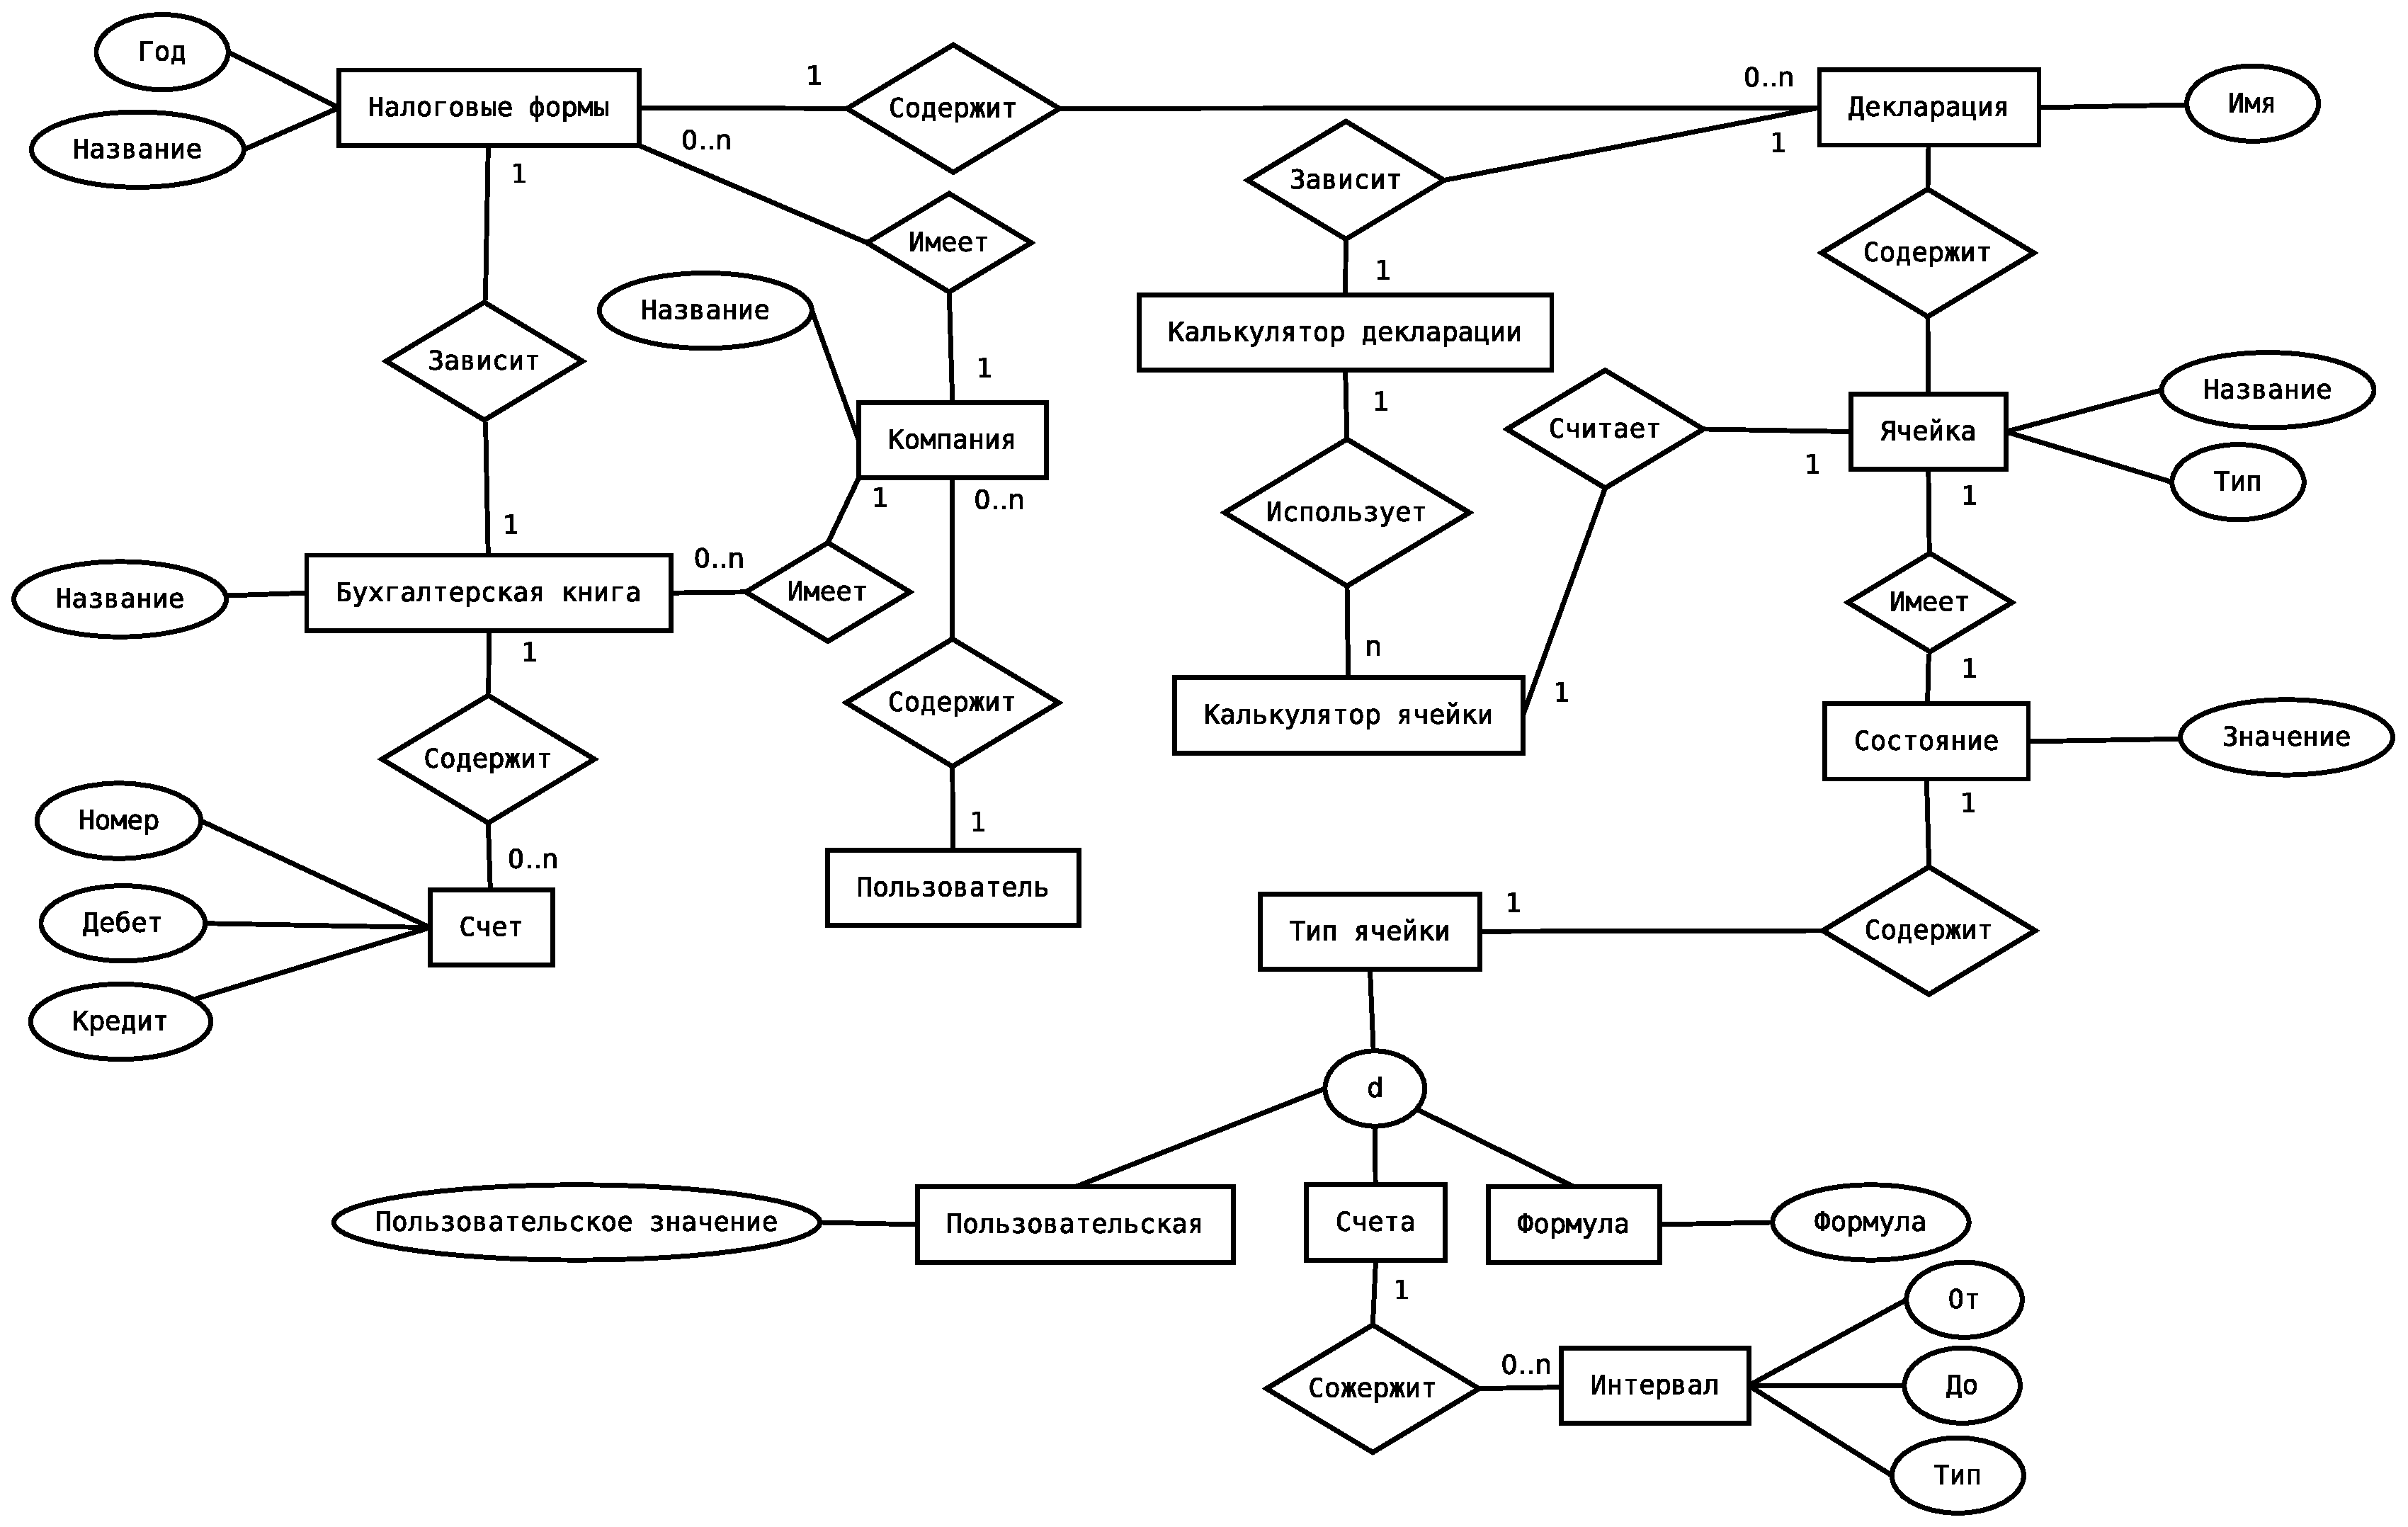
\includegraphics[scale=0.4]{uml/entity_pretty}
  \caption{Диаграмма сущность-связь}
  \label{pic:er_diagram}
\end{sidewaysfigure}

Отразим взаимодействие пользователя с сущностями системы на диаграммах вариантов использования. Пользователем системы будет являться человек, занимающий должность в организации, ответственную за заполнение налоговых деклараций и ведение бухгалтерии, в общем случае - это бухгалтер, по этому в качестве первостепенного актера на диаграммах вариантов использования будем использовать <<Бухгалтера>>.

Рассмотрим диаграмму вариантов использования для работы с <<Компанией>>. Пользователь может создавать новую компанию, может редактировать и удалить существующую (рисунок~\ref{pic:use_case_4}).

На рисунке~\ref{pic:use_case_3} приведена диаграмма вариантов использования для работы с <<Бухгалтерской книгой>>, пользователь может создавать <<Бухгалтерскую книгу>>, может её редактировать, при редактировании возможно добавление, удаление и редактирования <<Счетов>>, так же пользователь может удалить уже существующую <<Бухгалтерскую книгу>>.

Изобразим варианты использования для работы с <<Набором деклараций>> (рисунок~\ref{pic:use_case_2}), пользователь может создать, редактировать и удалить уже существующий <<Набор деклараций>>.

Рассмотрим варианты использования для работы <<Декларацией>> (рисунок~\ref{pic:use_case_1}). <<Бухгалтер>> является пользователем системы, <<Калькулятор декларации>> и <<Калькулятор ячейки>> - сущности системы, которые выполняют действия, необходимые для подсчета всей декларации и одной ячейки соответственно. <<Бухгалтер>> открывает декларацию, <<Калькулятор декларации>> подсчитывает открываемую декларацию. <<Бухгалтер>> может пересчитать значение ячейки, изменить тип значения ячейки - задать другой тип ячейки из возможных, либо изменить параметр ячейки, данные действия вызывают пересчет ячейки, за что отвечает <<Калькулятор ячейки>>.

\begin{figure}
  \centering
  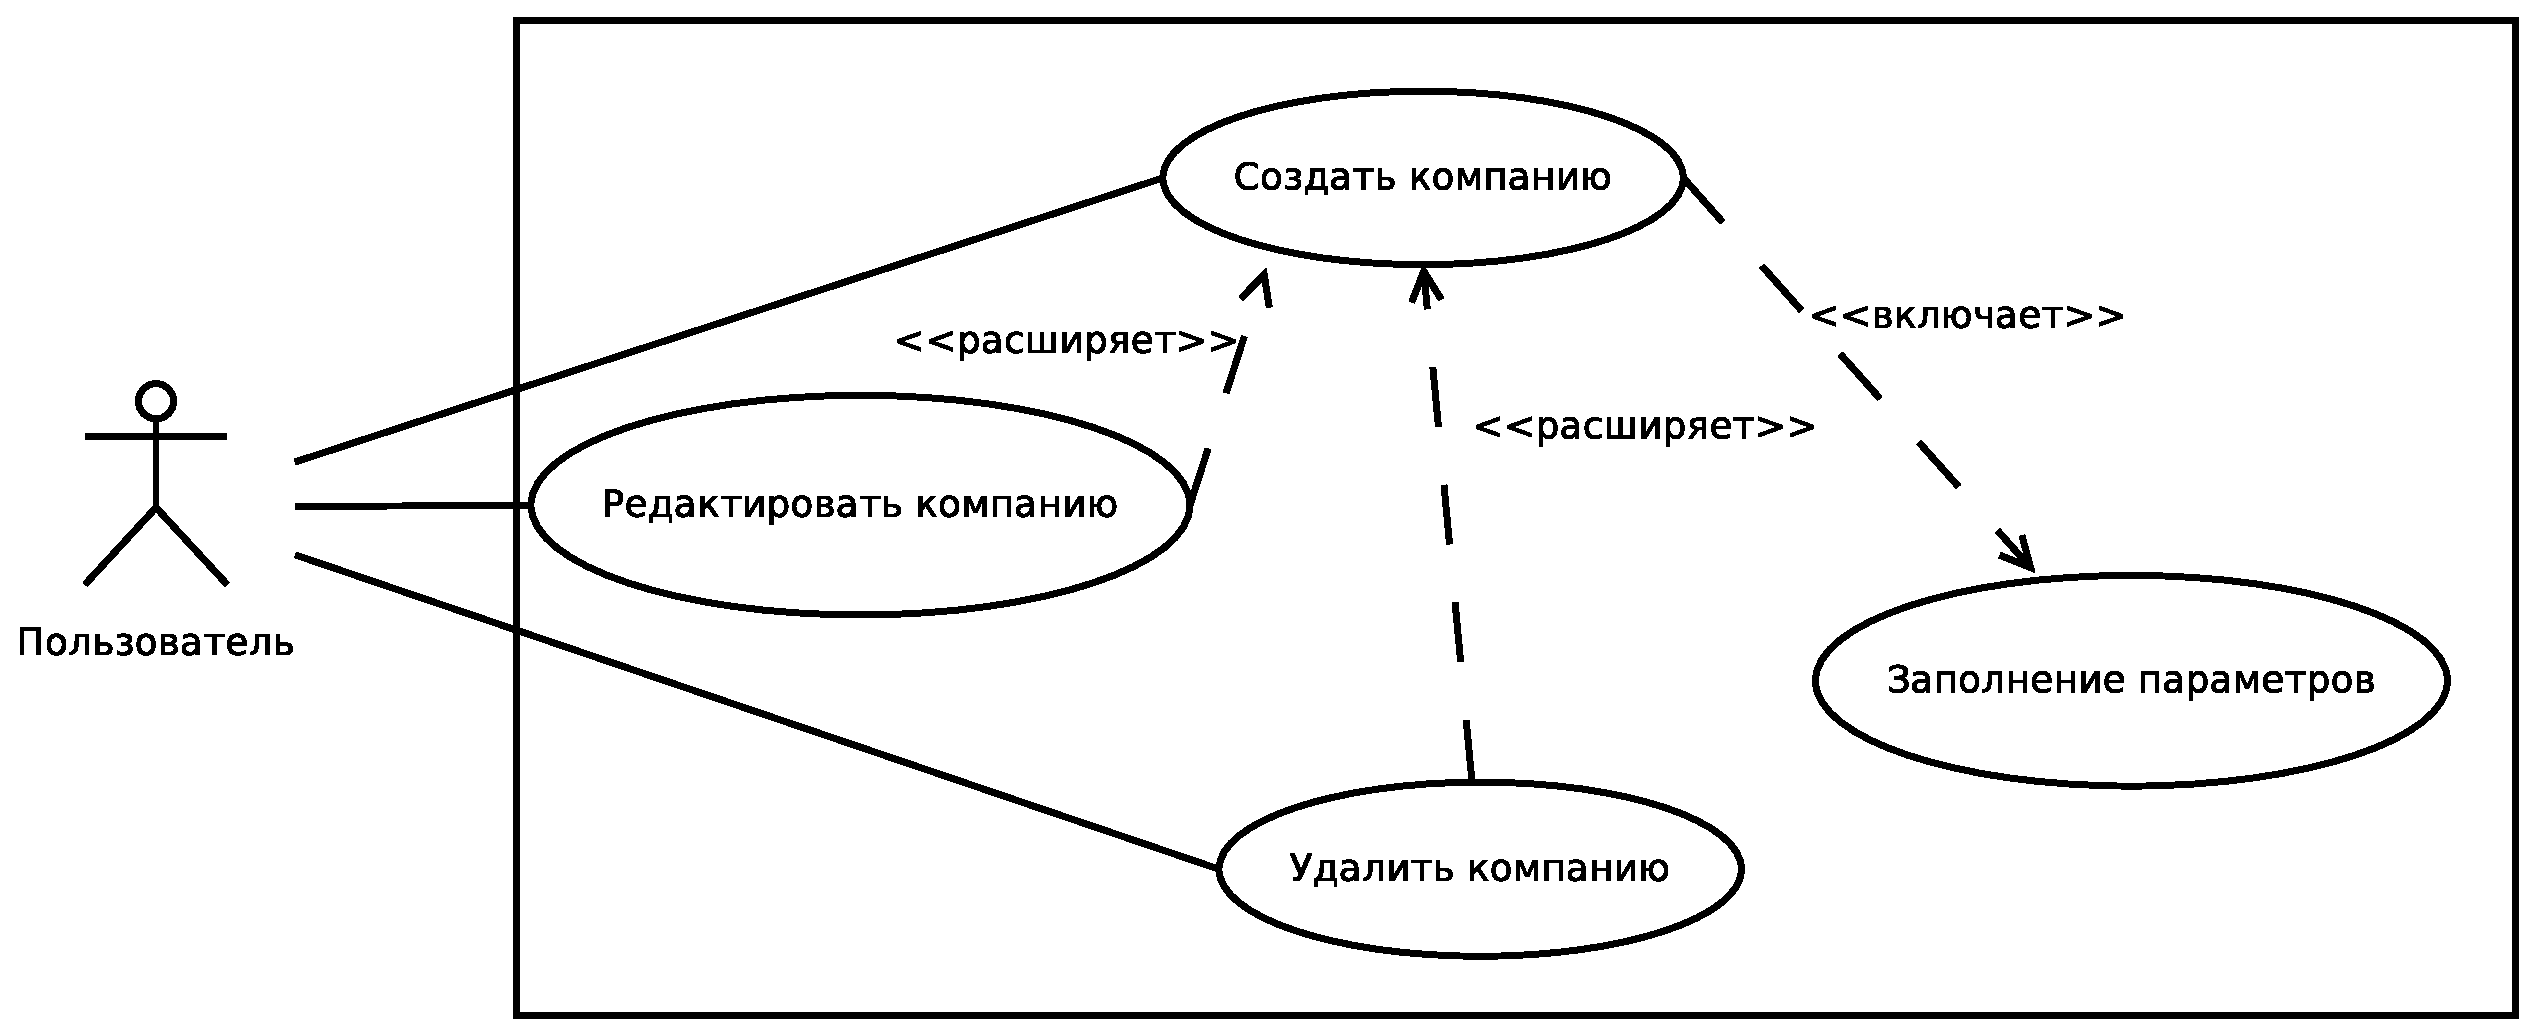
\includegraphics[scale=0.4]{uml/usecase_4}
  \caption{Диаграмма вариантов использования для работы с компанией}
  \label{pic:use_case_4}
\end{figure}

\begin{figure}
  \centering
  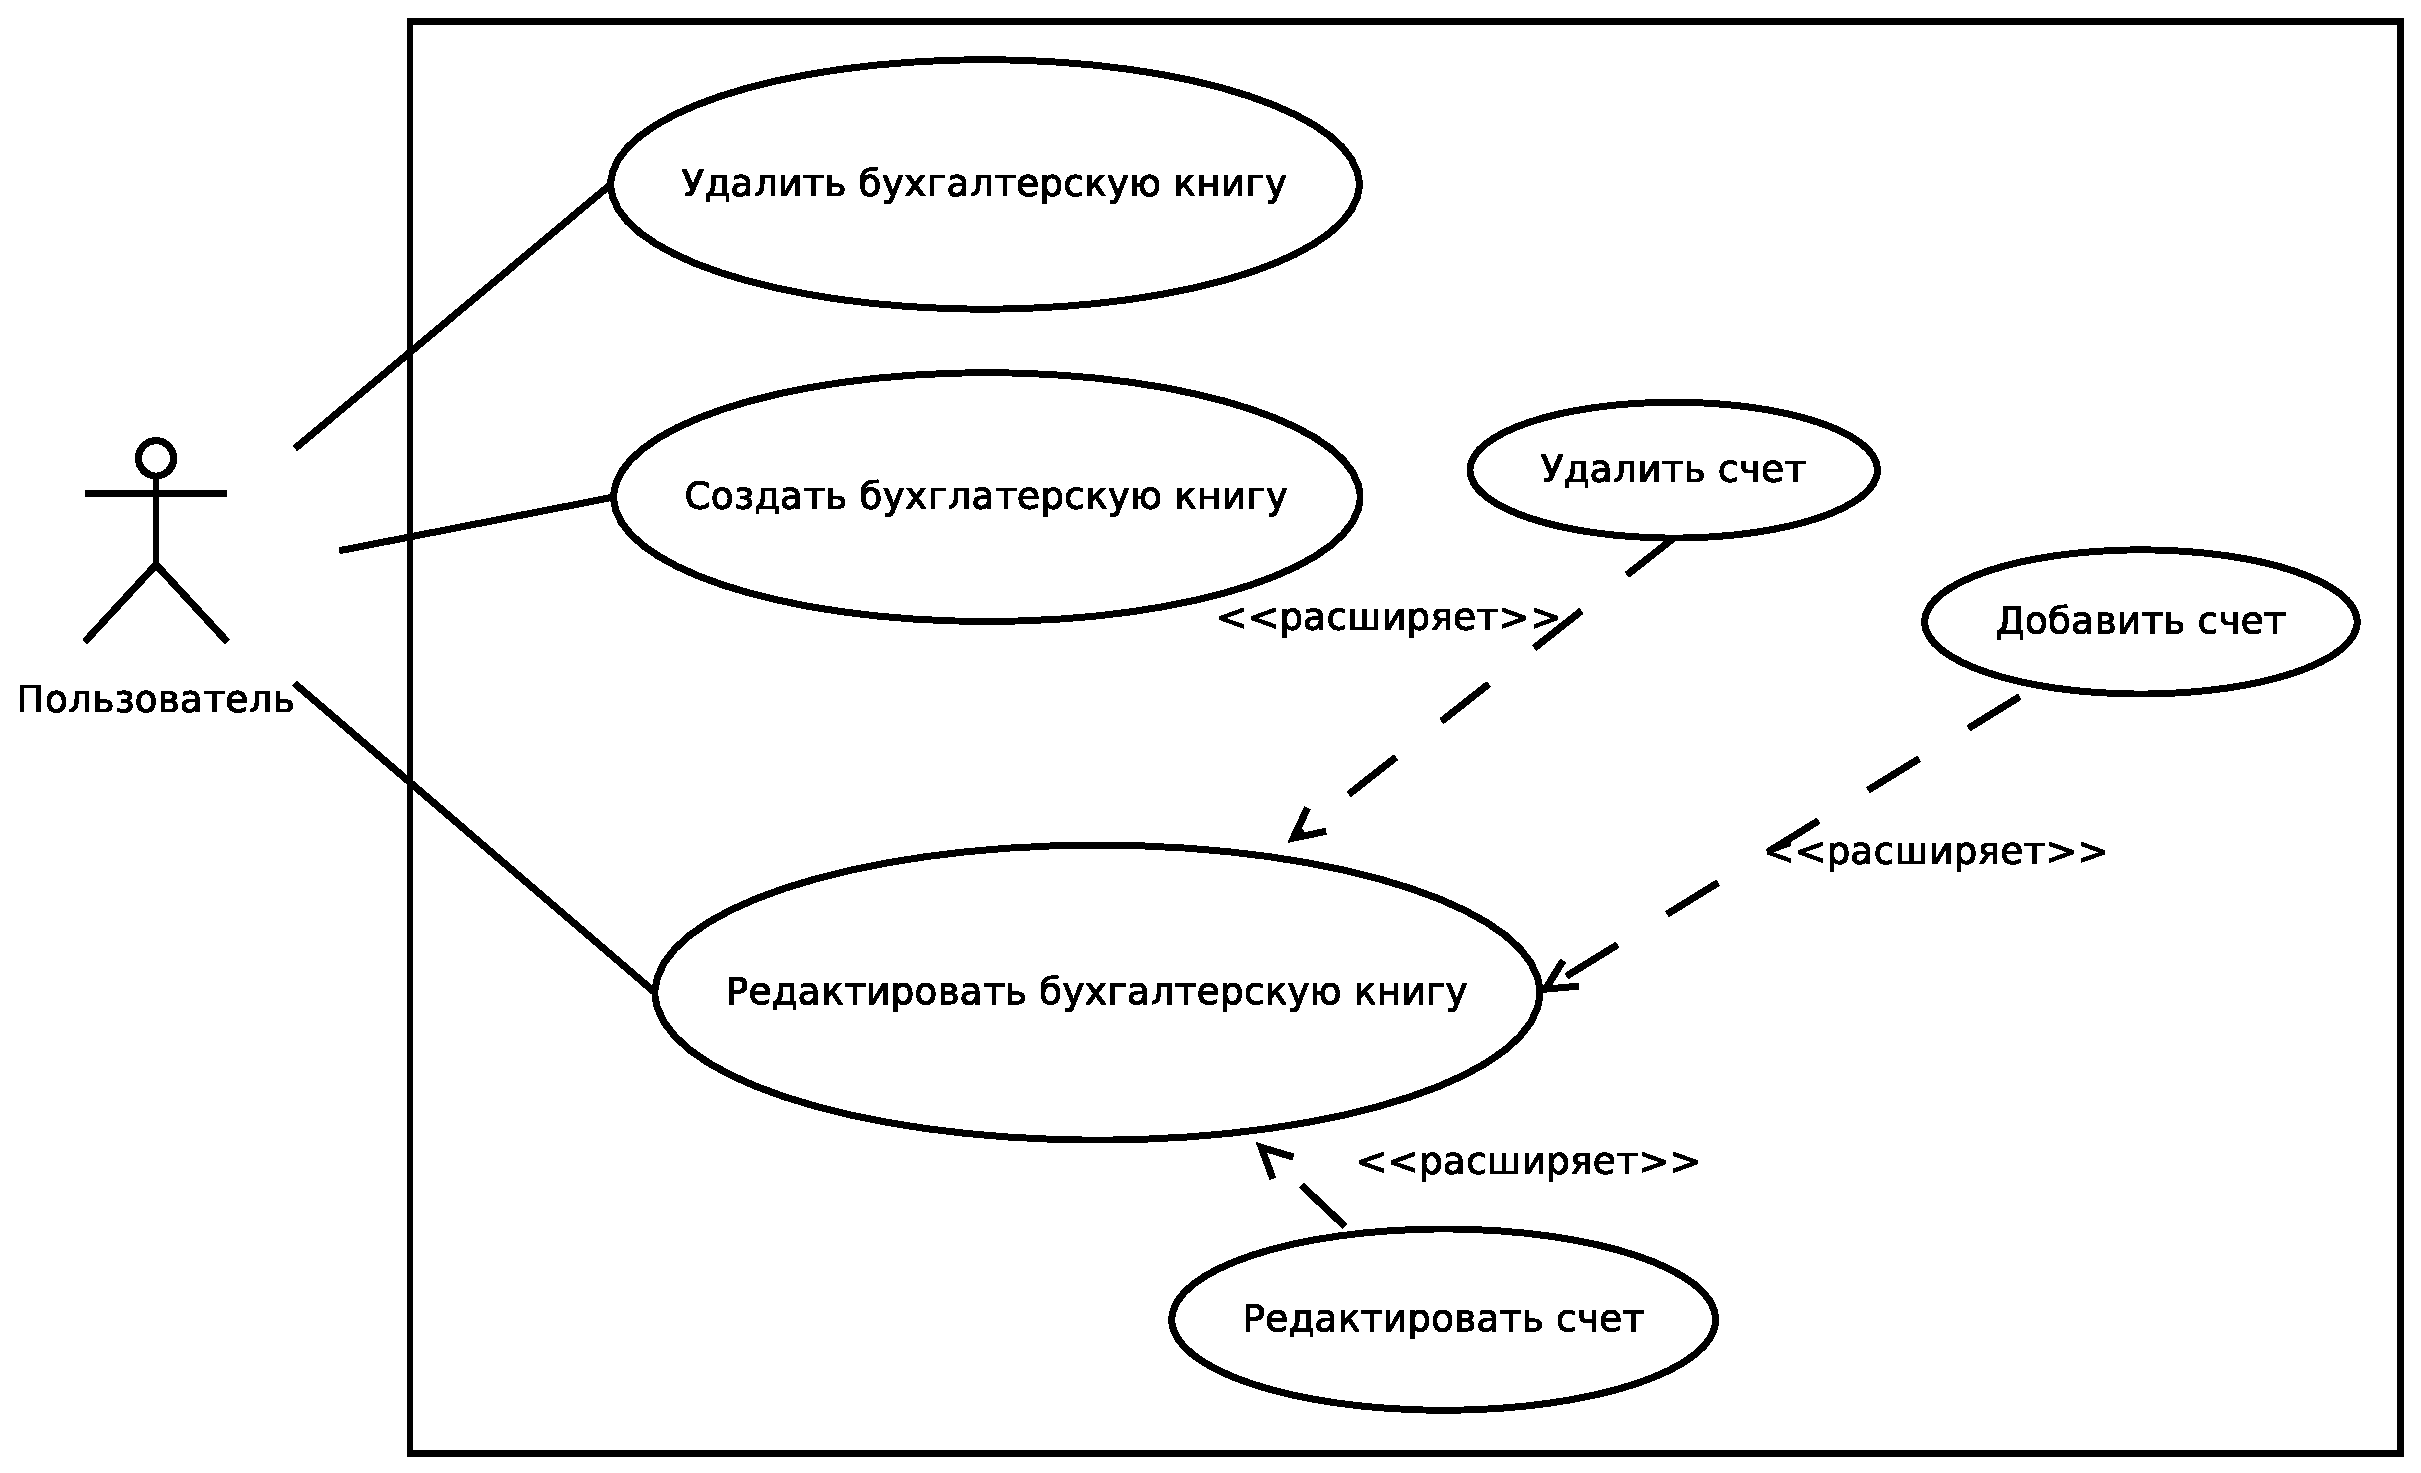
\includegraphics[scale=0.4]{uml/usecase_3}
  \caption{Диаграмма вариантов использования для работы с бухгалтерской книгой}
  \label{pic:use_case_3}
\end{figure}

\begin{figure}
  \centering
  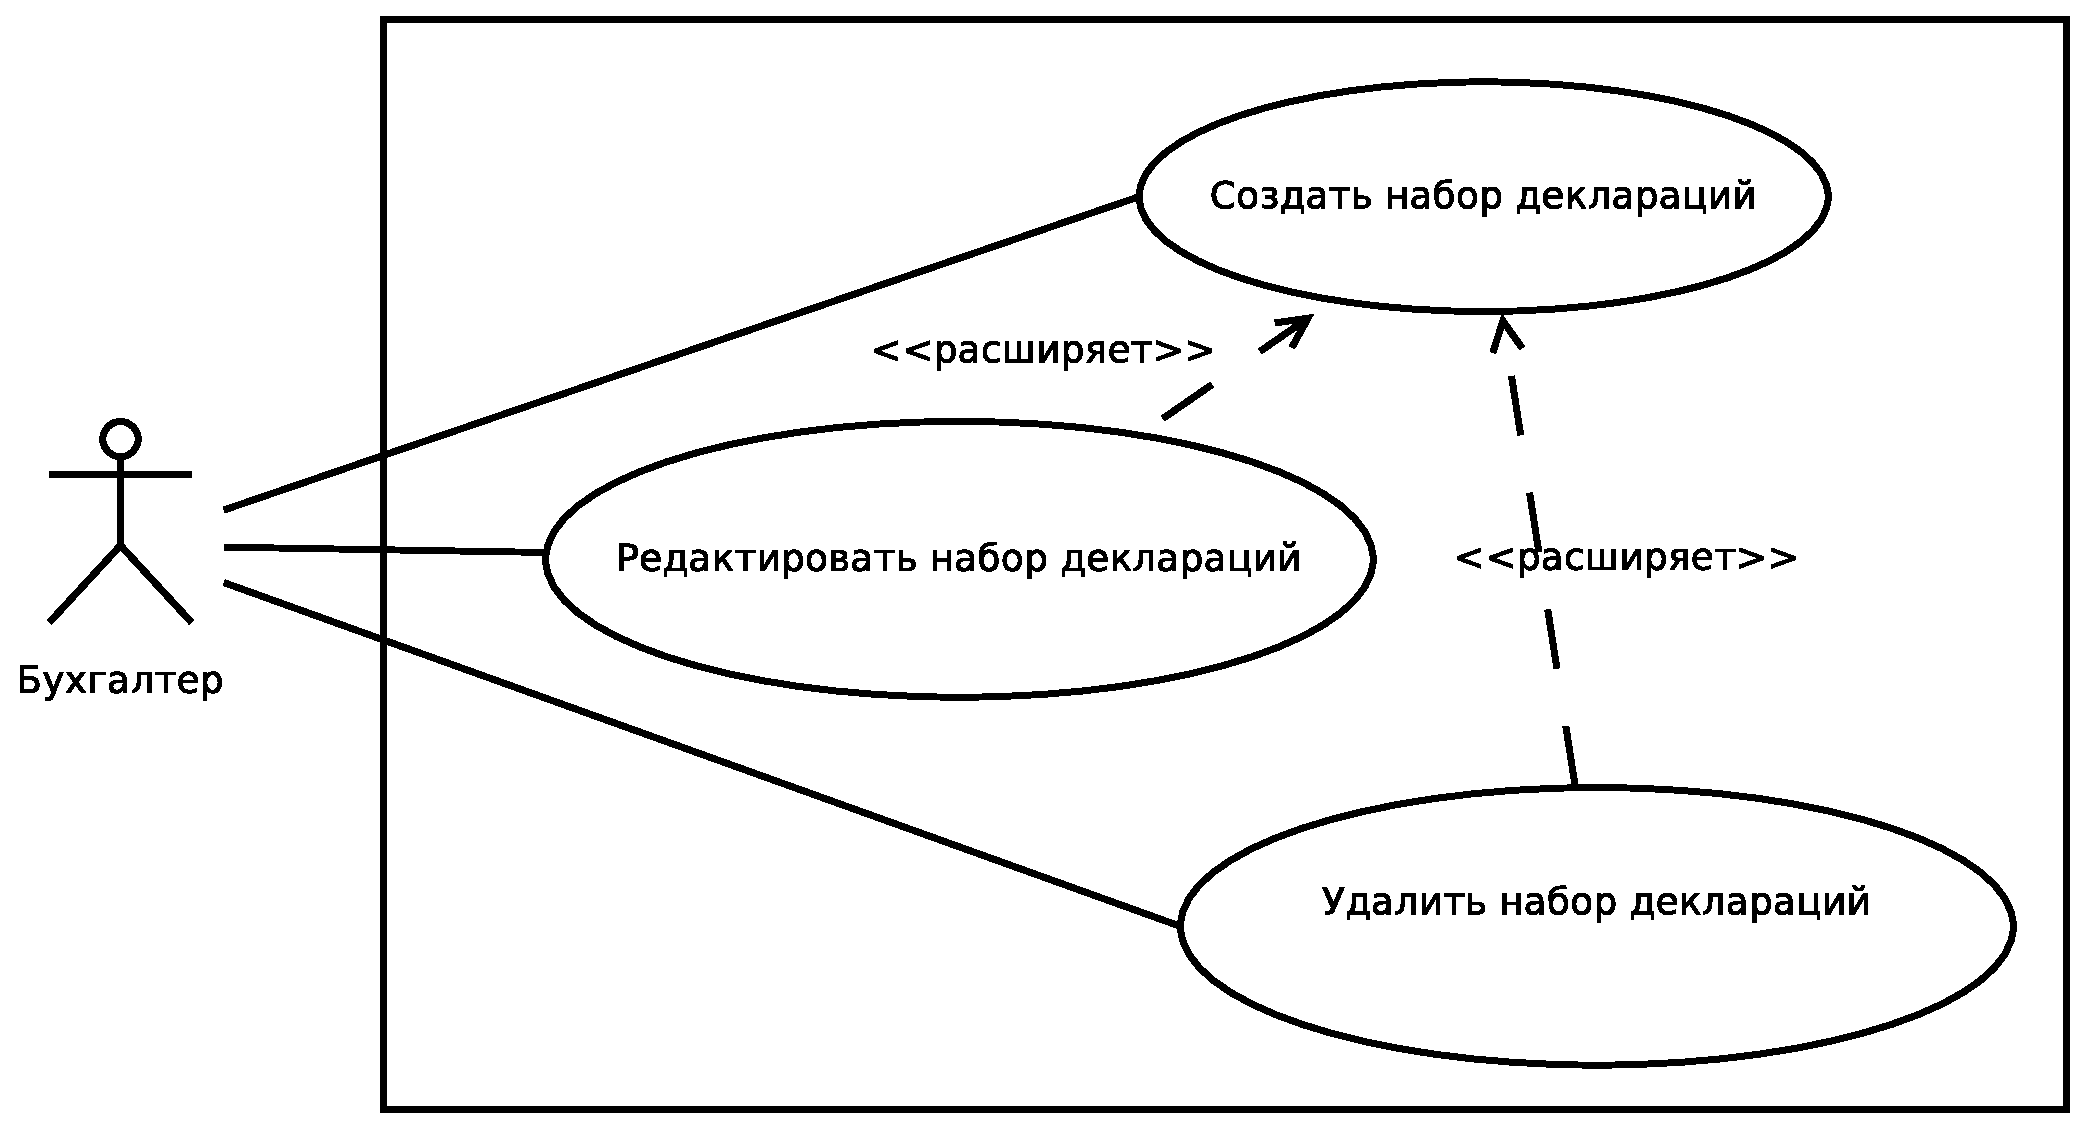
\includegraphics[scale=0.4]{uml/usecase_2}
  \caption{Диаграмма вариантов использования для работы с набором деклараций}
  \label{pic:use_case_2}
\end{figure}

\begin{sidewaysfigure}
  \centering
  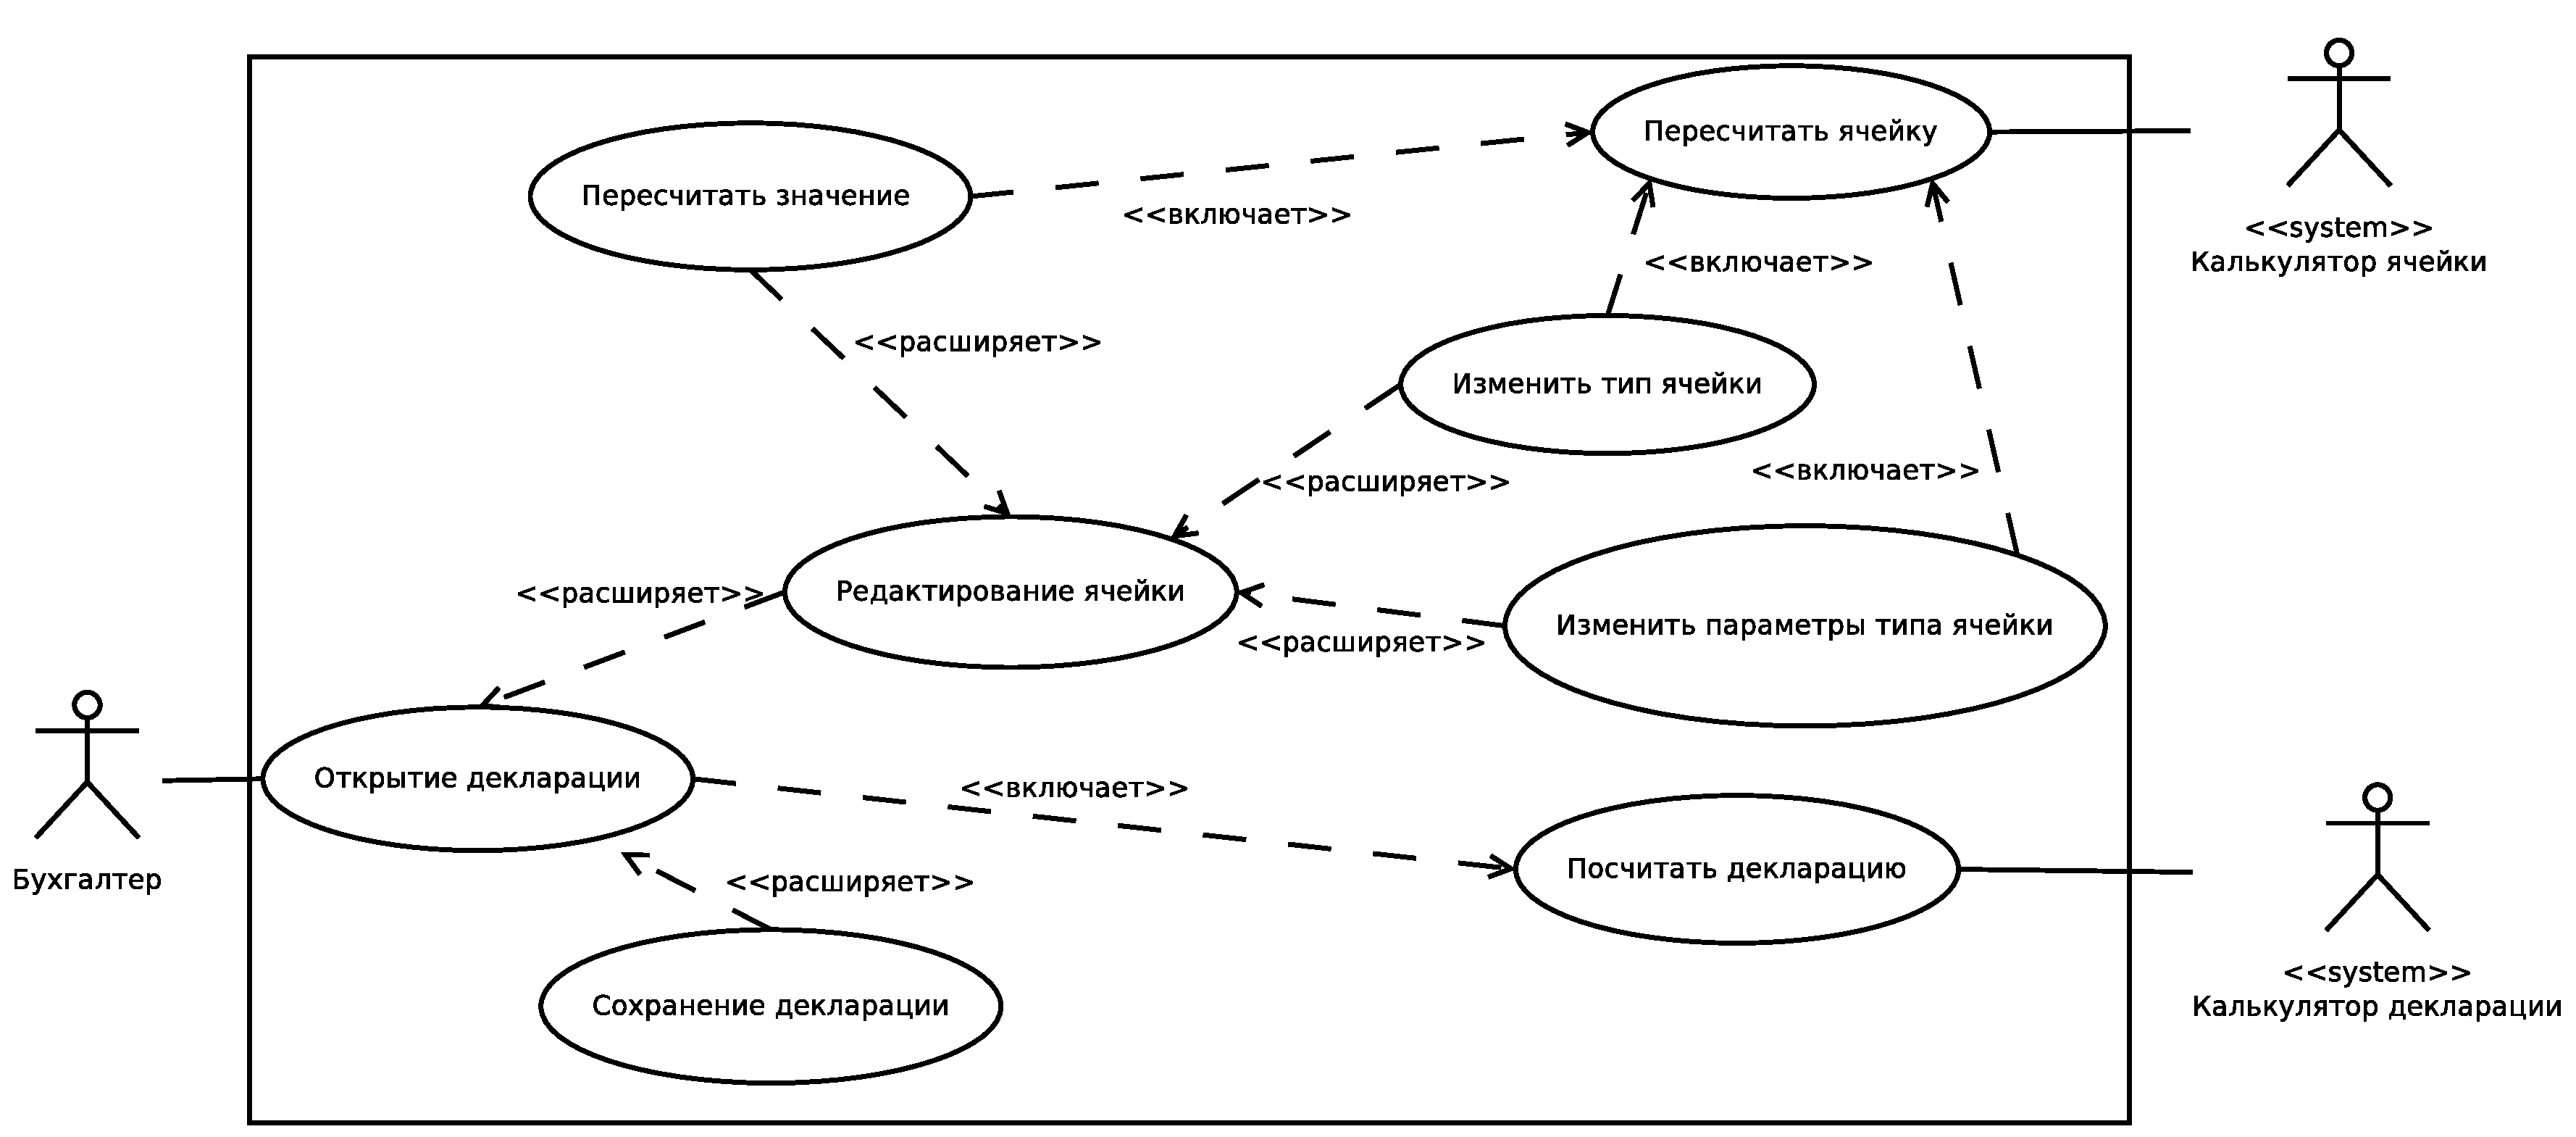
\includegraphics[scale=0.4]{uml/usecase_1}
  \caption{Диаграмма вариантов использования для работы с декларацией}
  \label{pic:use_case_1}
\end{sidewaysfigure}

Для отражения взаимодействия объектов системы приведем диаграммы последовательности.

Приведем диаграмму последовательности для вариантов использования при работе с компанией (рисунок~\ref{pic:sequence_1}).  Класс <<Сервис компании>> будет отвечать за работу с базой данных для объекта <<Компания>>. При создании компании пользователь должен заполнить форму создания компании, затем <<Сервис компании>> сохранит созданную компанию. Для редактирования <<Сервис компании>> загружает сохраненную компанию, затем пользователь посредством формы редактирования изменяет параметры и <<Сервис компании>> сохраняет загруженный объект с новыми параметрами. Для удаления компании пользователь выбирает из списка существующих компаний компанию, которую он хочет удалить, <<Сервис компании>> удаляет выбранную пользователем компанию из базы данных.

\begin{figure}
  \centering
  \includegraphics[scale=0.4]{uml/_sequence_4}
  \caption{Диаграмма последовательности для компании}
  \label{pic:sequence_1}
\end{figure}

Приведем диаграмму последовательности для работы с бухгалтерской книгой (рисунок~\ref{pic:sequence_2}). Пользователь создает бухгалтерскую книгу посредством формы создания, далее задает параметры для объекта, после чего значения параметров устанавливаются у созданного объекта <<Бухгалтерская книга>>. При добавлении пользователем нового счета создается объект <<Счет>> и добавляется в <<Бухгалтерскую книгу>>. При удалении счета на форме, счет удаляется из созданного объекта <<Бухгалтерская книга>>. При изменении параметров счета на форме, параметры счета изменяются в созданном объекте <<Бухгалтерская книга>>. За сохранение <<Бухгалтерской книги>> в базе данных отвечает класс <<Сервис Бухгалтерской книги>>.

\begin{sidewaysfigure}
  \centering
  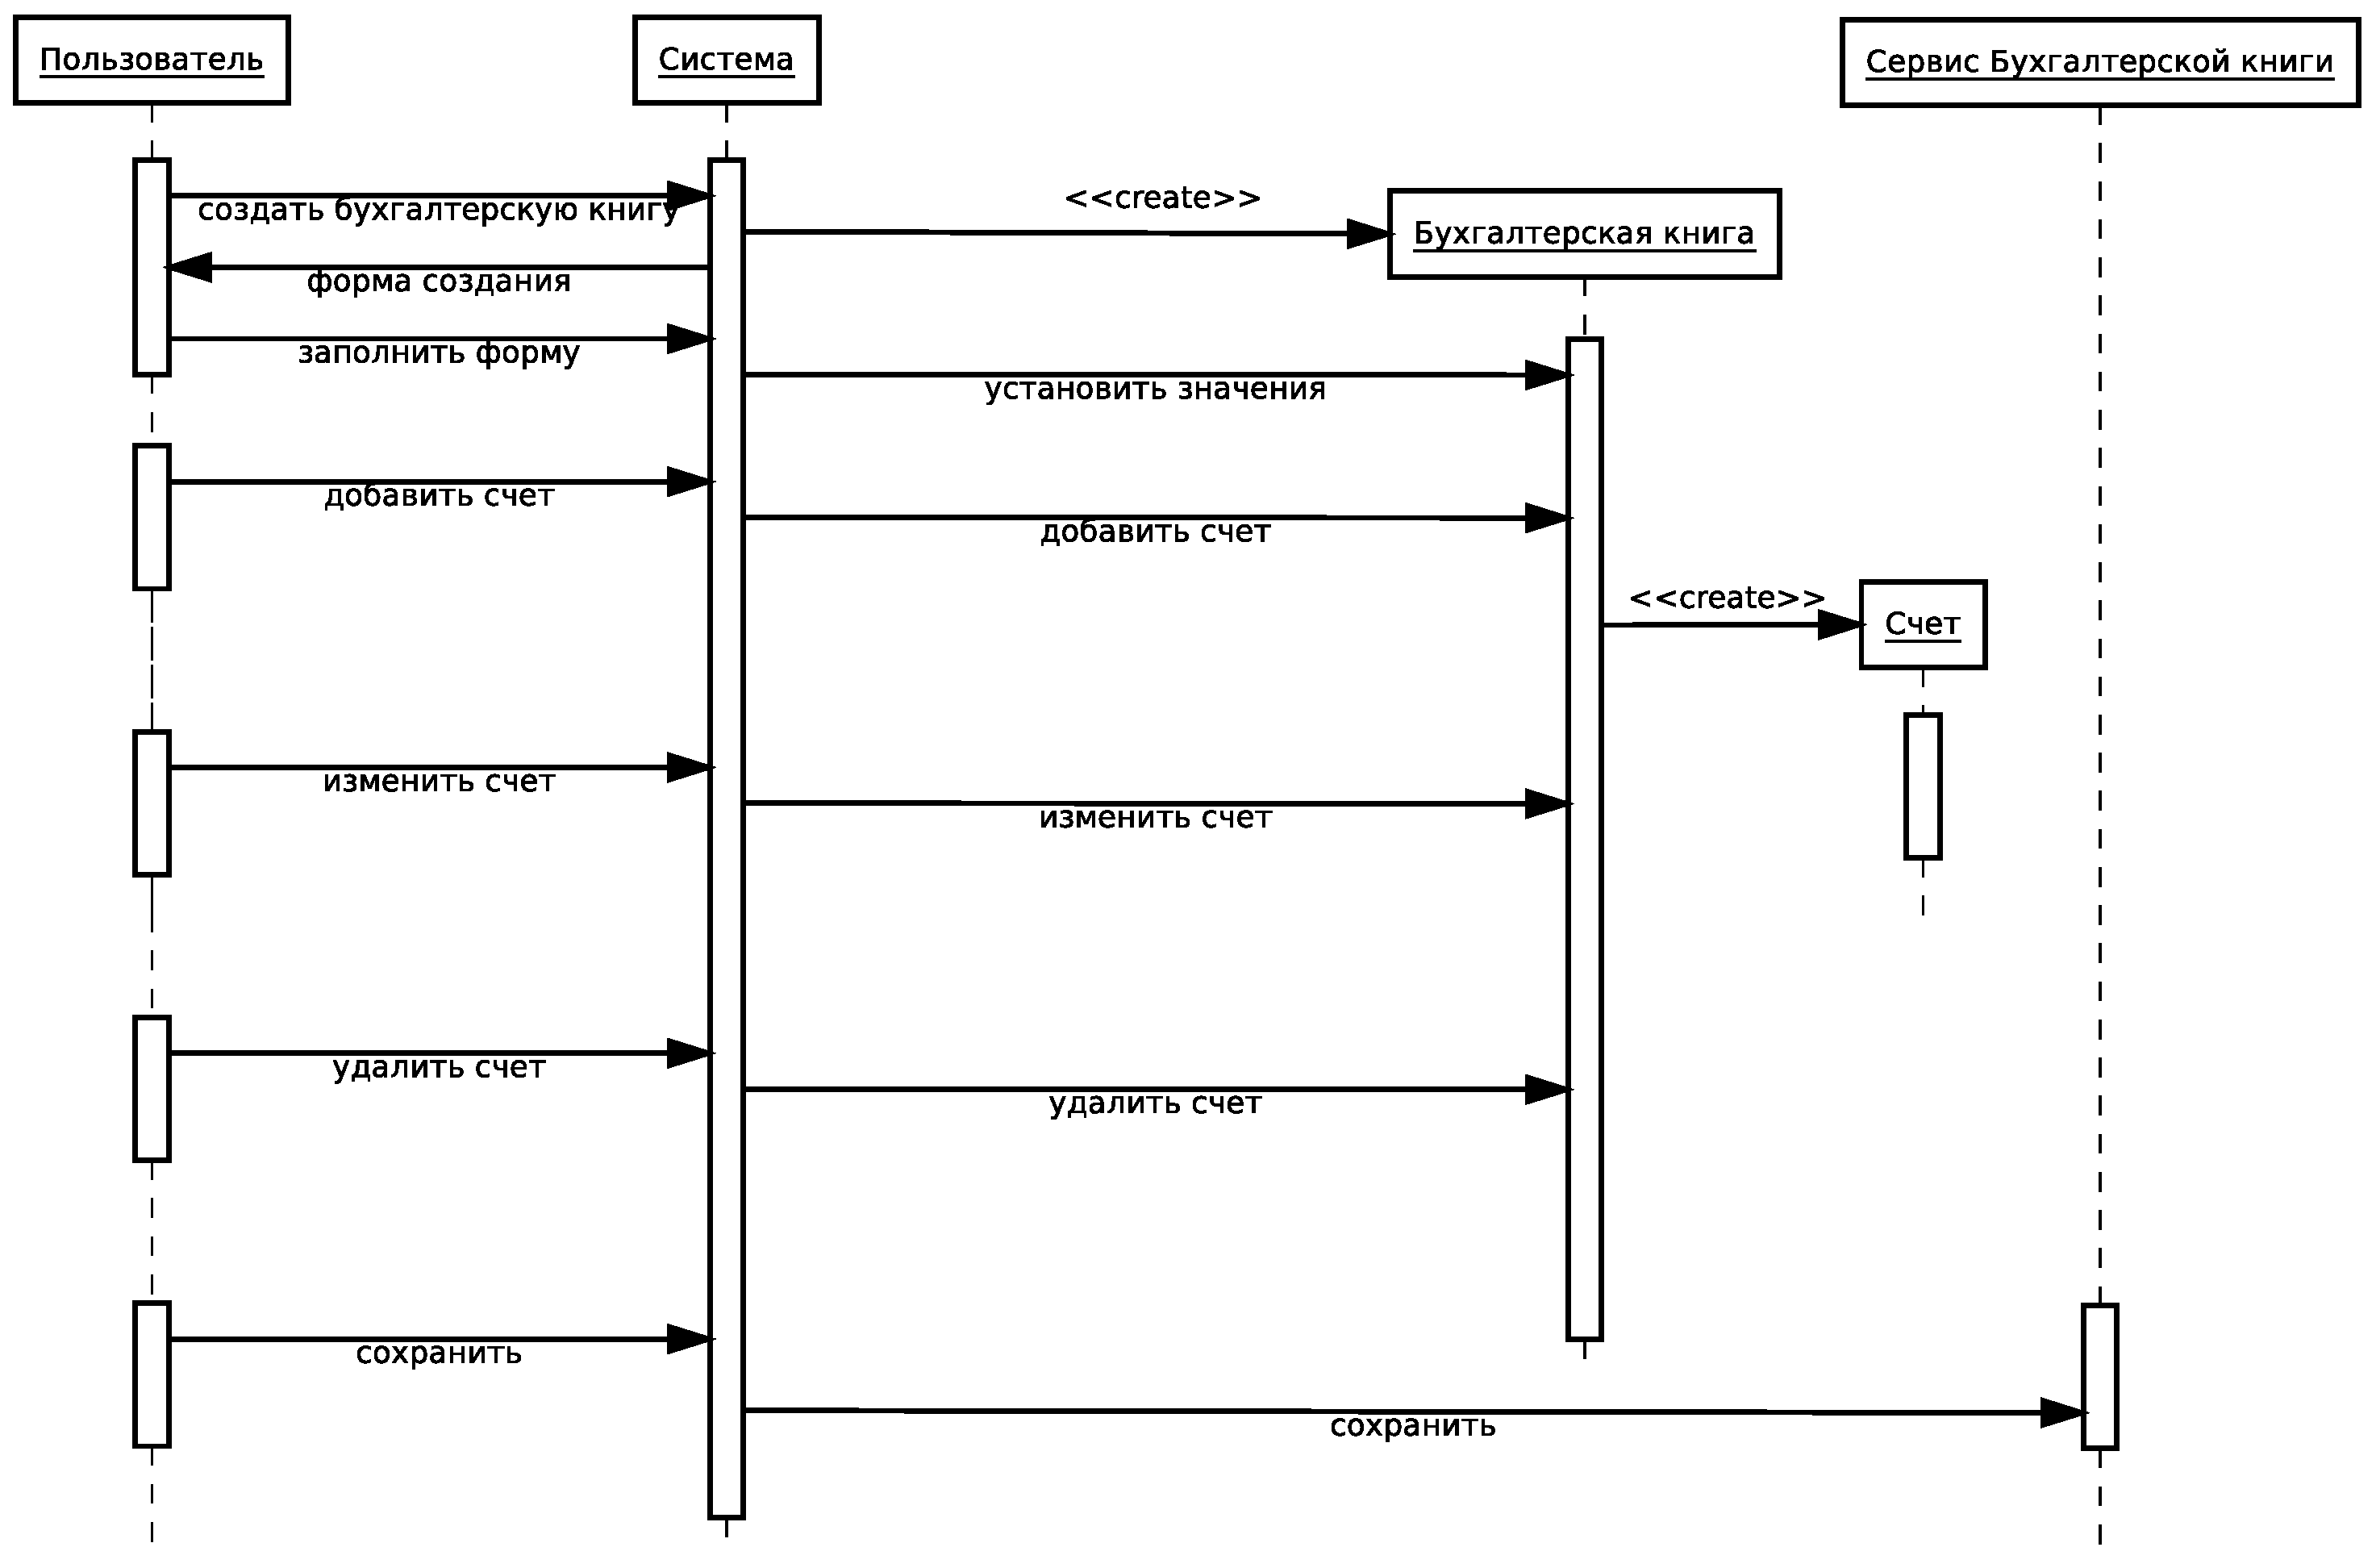
\includegraphics[scale=0.4]{uml/_sequence_5}
  \caption{Диаграмма последовательности для бухгалтерской книги}
  \label{pic:sequence_2}
\end{sidewaysfigure}

Приведем диаграмму последовательности для работы с налоговыми формами. Класс <<Сервис Налоговых форм>> будет отвечать за работу с базой данных для объекта <<Налоговые формы>>. При создании налоговых форм пользователь должен заполнить форму необходимыми параметрами, во время создания пользователем налоговых форм создается объект <<Налоговые формы>>. Посредством пользовательского интерфейса, пользователь задает параметры, после того как параметры заданы, объект <<Налоговые формы>> сохраняется в базе данных, за сохранение отвечает объект <<Сервис Налоговых форм>>. Для редактирования налоговые формы загружаются из базы данных при помощи объекта <<Сервис Налоговых форм>>. Далее, посредством интерфейса пользователя, пользователь изменяет параметры объекта, после чего объект <<Сервис Налоговых форм>> сохраняет измененный объект в базе данных. Для удаления, пользователю необходимо выбрать нужные налоговые формы, класс <<Сервис Налоговых форм>> удалит формы из базы данных.

\begin{figure}
  \centering
  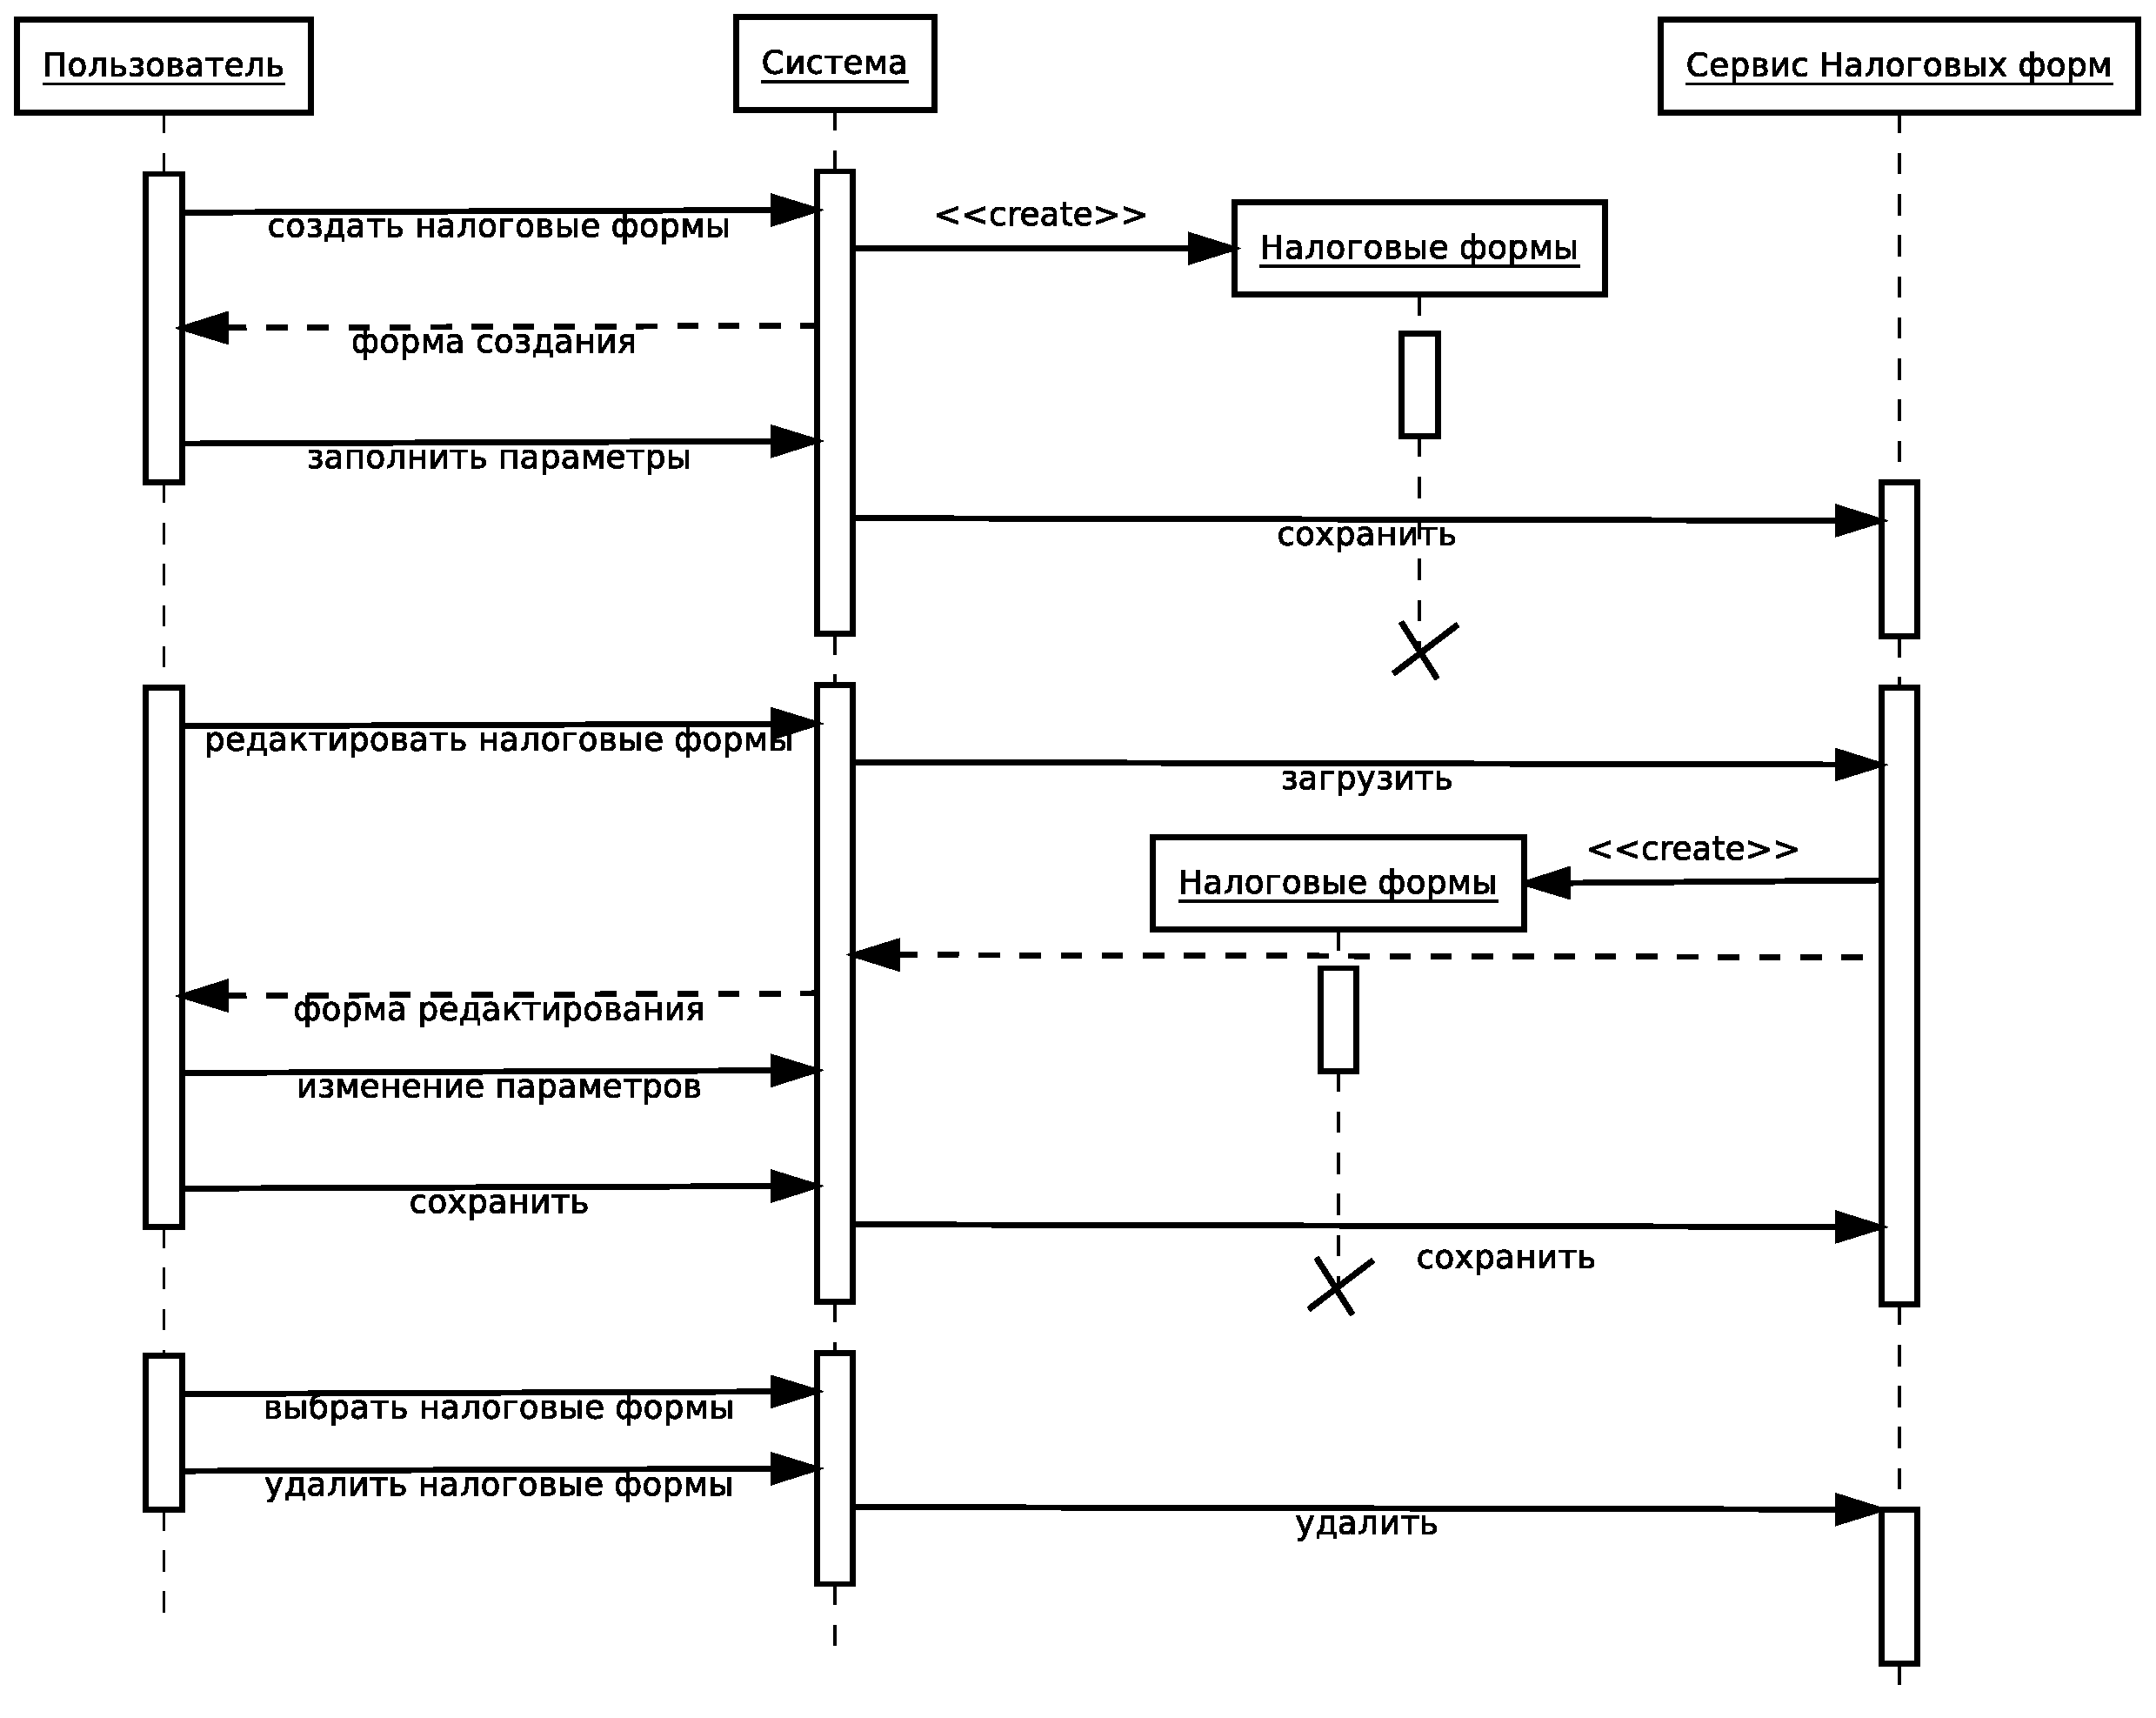
\includegraphics[scale=0.4]{uml/_sequence_6}
  \caption{Диаграмма последовательности для налоговых форм}
  \label{pic:sequence_3}
\end{figure}

Приведем диаграмму последовательности для открытия декларации (рисунок~\ref{pic:sequence_4}). Введем новый класс <<Сервис декларации>>, который будет отвечать за работу с <<Декларацией>>: загрузка структуры декларации (ячейки, типы ячеек, параметры типов ячеек <<по умолчанию>>) и загрузку состояния декларации (значения ячеек, параметры типов ячеек). <<Сервис декларации>> при загрузке декларации создает объект <<Декларация>> и, если декларация уже была сохранена (открыта не первый раз), устанавливает сохраненное состояние. После загрузки декларации, <<Калькулятор декларации>> подсчитывает значение ячеек декларации (и устанавливает значения ячеек). Далее <<Пользовательский интерфейс>> отображает декларацию.

\begin{figure}
  \centering
  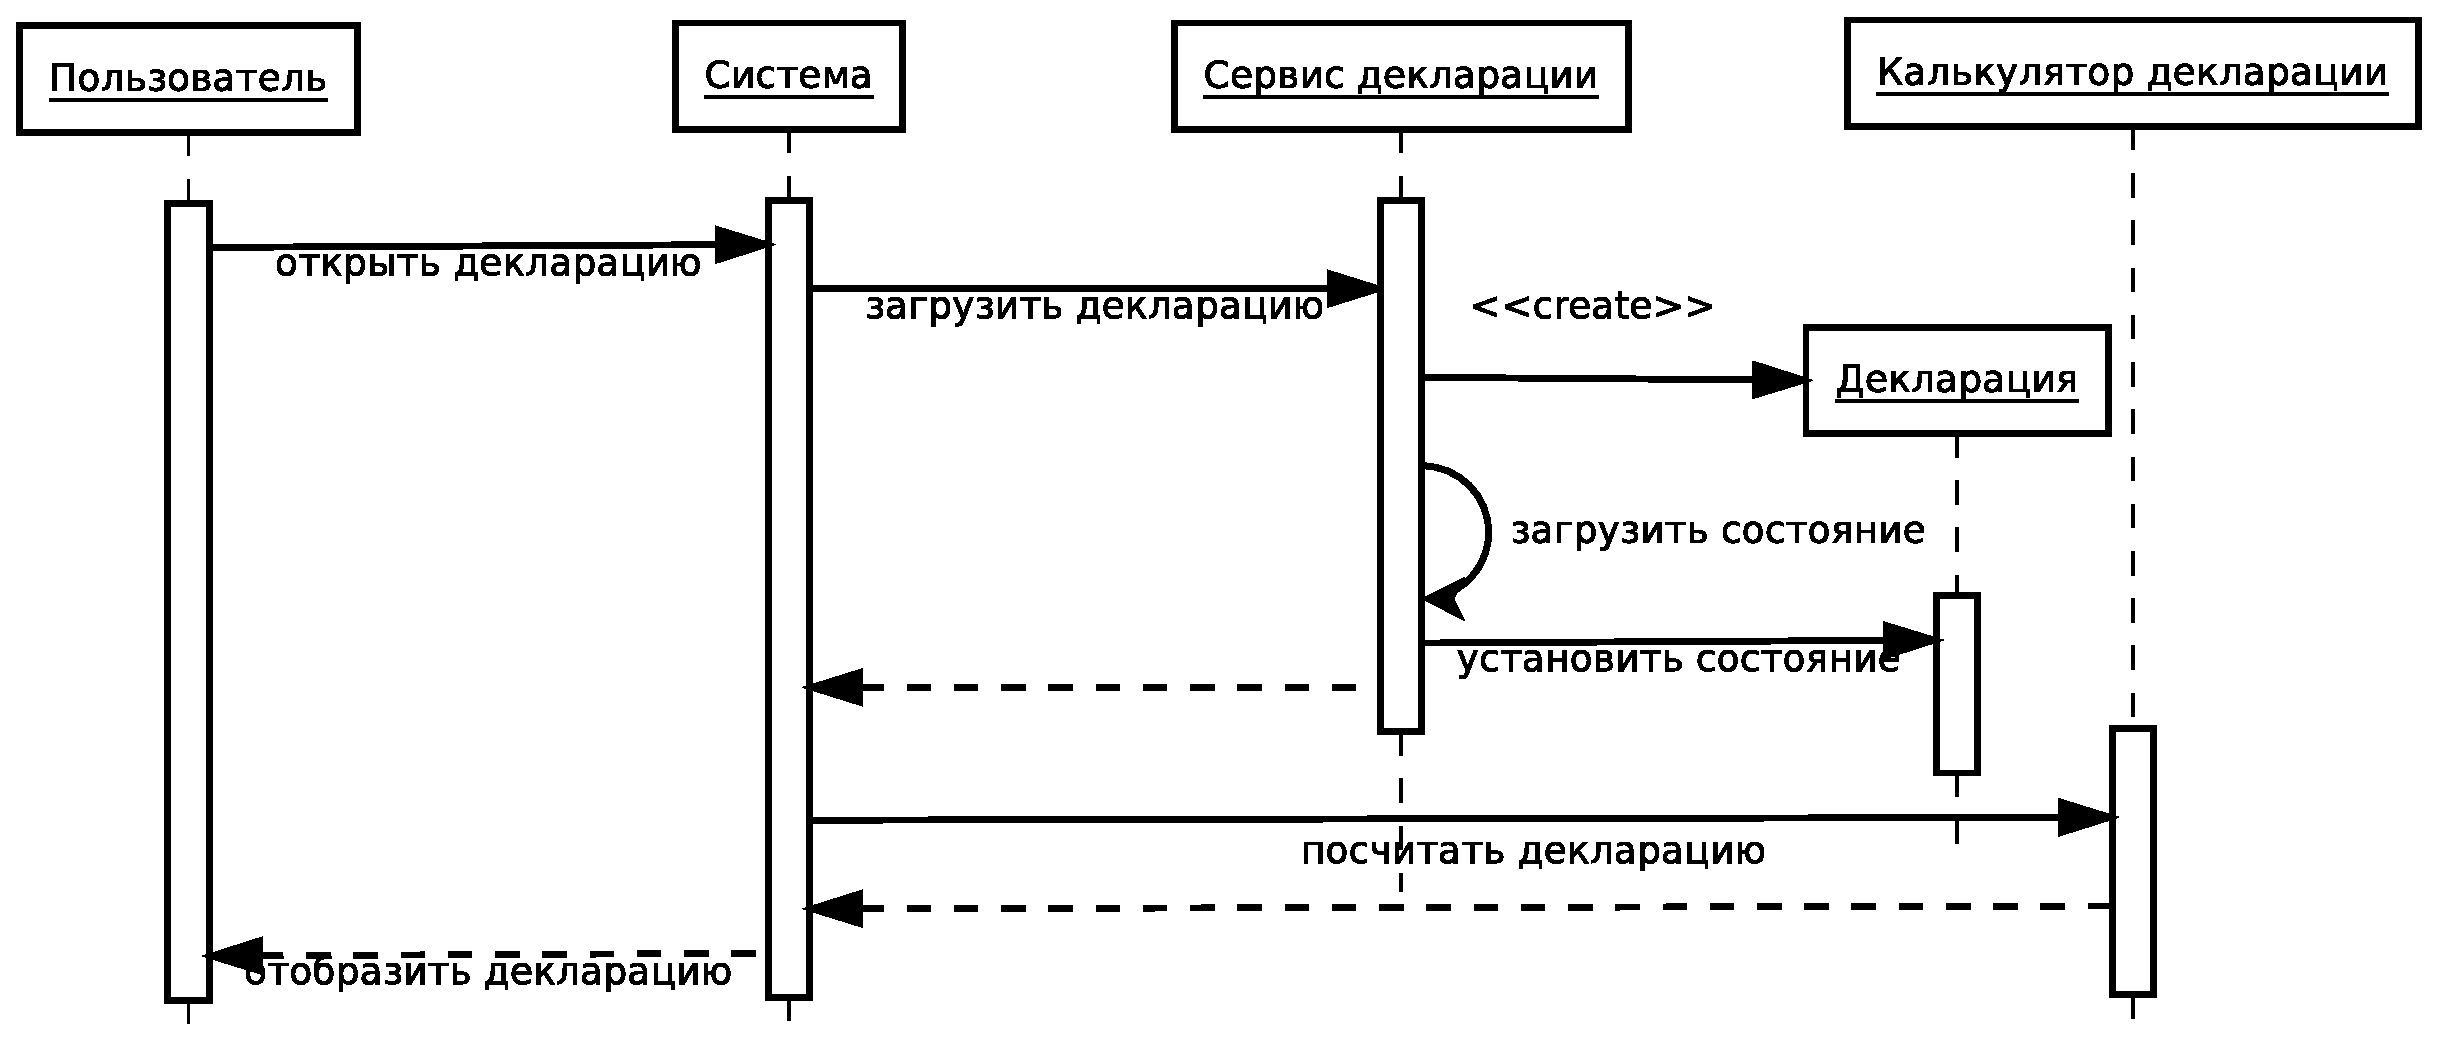
\includegraphics[scale=0.4]{uml/_sequence_1}
  \caption{Диаграмма последовательности для открытия декларации}
  \label{pic:sequence_4}
\end{figure}

На рисунке \ref{pic:sequence_4_} изображена диаграмма последовательности для редактирования ячейки. Изменение типа ячейки происходит установкой типа <<Состояния ячейки>>. После изменения типа ячейки необходим пересчет ячейки, который производится <<Калькулятором ячейки>>. Изменение параметров типа ячейки происходит с помощью установки параметров объекта <<Состояние ячейки>>, после установки новых параметров ячейка пересчитывается <<Калькулятором ячейки>>.

\begin{sidewaysfigure}
  \centering
  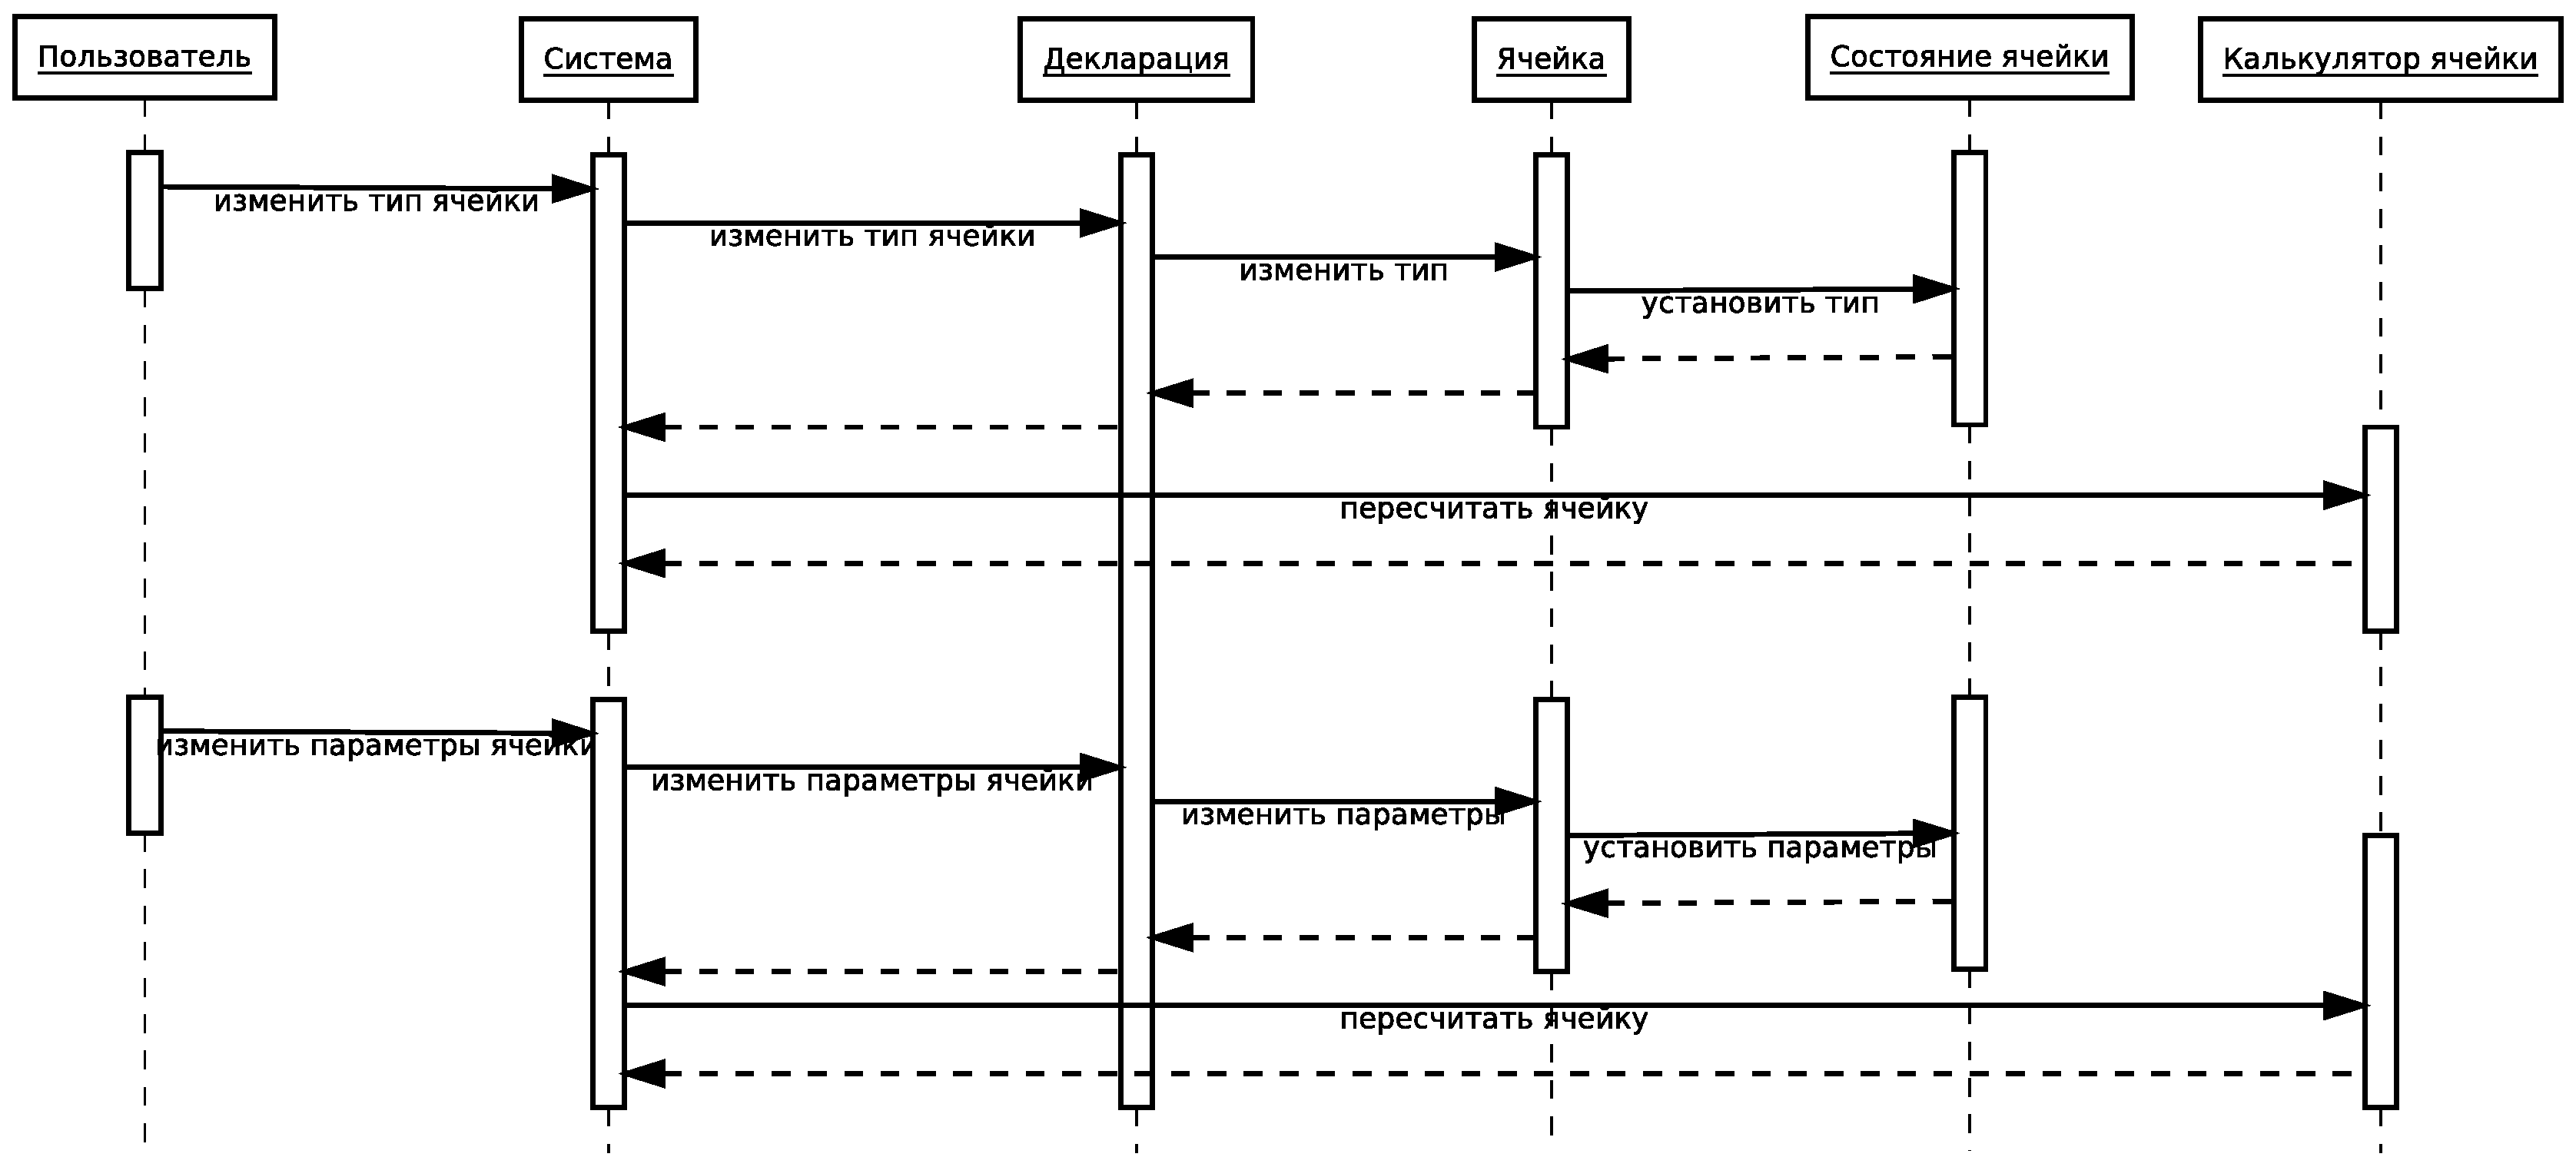
\includegraphics[scale=0.4]{uml/_sequence_2}
  \caption{Диаграмма последовательности для редактирования ячейки}
  \label{pic:sequence_4_}
\end{sidewaysfigure}

Небольшая диаграмма последовательности для сохранения декларации приведена на рисунке \ref{pic:sequence_5}. Пользователь сообщает системе о том, что хочет сохранить декларацию, <<Сервис декларации>> сохраняет декларацию.

\begin{figure}
  \centering
  \includegraphics[scale=0.4]{uml/_sequence_3}
  \caption{Диаграмма последовательности для сохранения декларации}
  \label{pic:sequence_5}
\end{figure}

Для представления о динамике поведения объектов в системе приведем диаграммы состояний. Рассмотрим диаграмму состояний для открытия декларации (рисунок \ref{pic:states_1}). При открытии декларации загружается структура декларации, которая содержит свойства декларации ( в данный момент выделено <<название>> ), список ячеек с их параметрами. Далее, осуществляется попытка загрузки уже сохраненного состояния, если пользователь открывал данную декларацию и сохранил её, то загружается сохраненное состояние, иначе создается состояние, с параметрами, определенными по умолчанию. Затем производится установка загруженных состояний, либо состояний созданных с параметрами, которые заданы по умолчанию. После того как состояния установлены, производиться подсчет значений ячеек декларации.

\begin{figure}
  \centering
  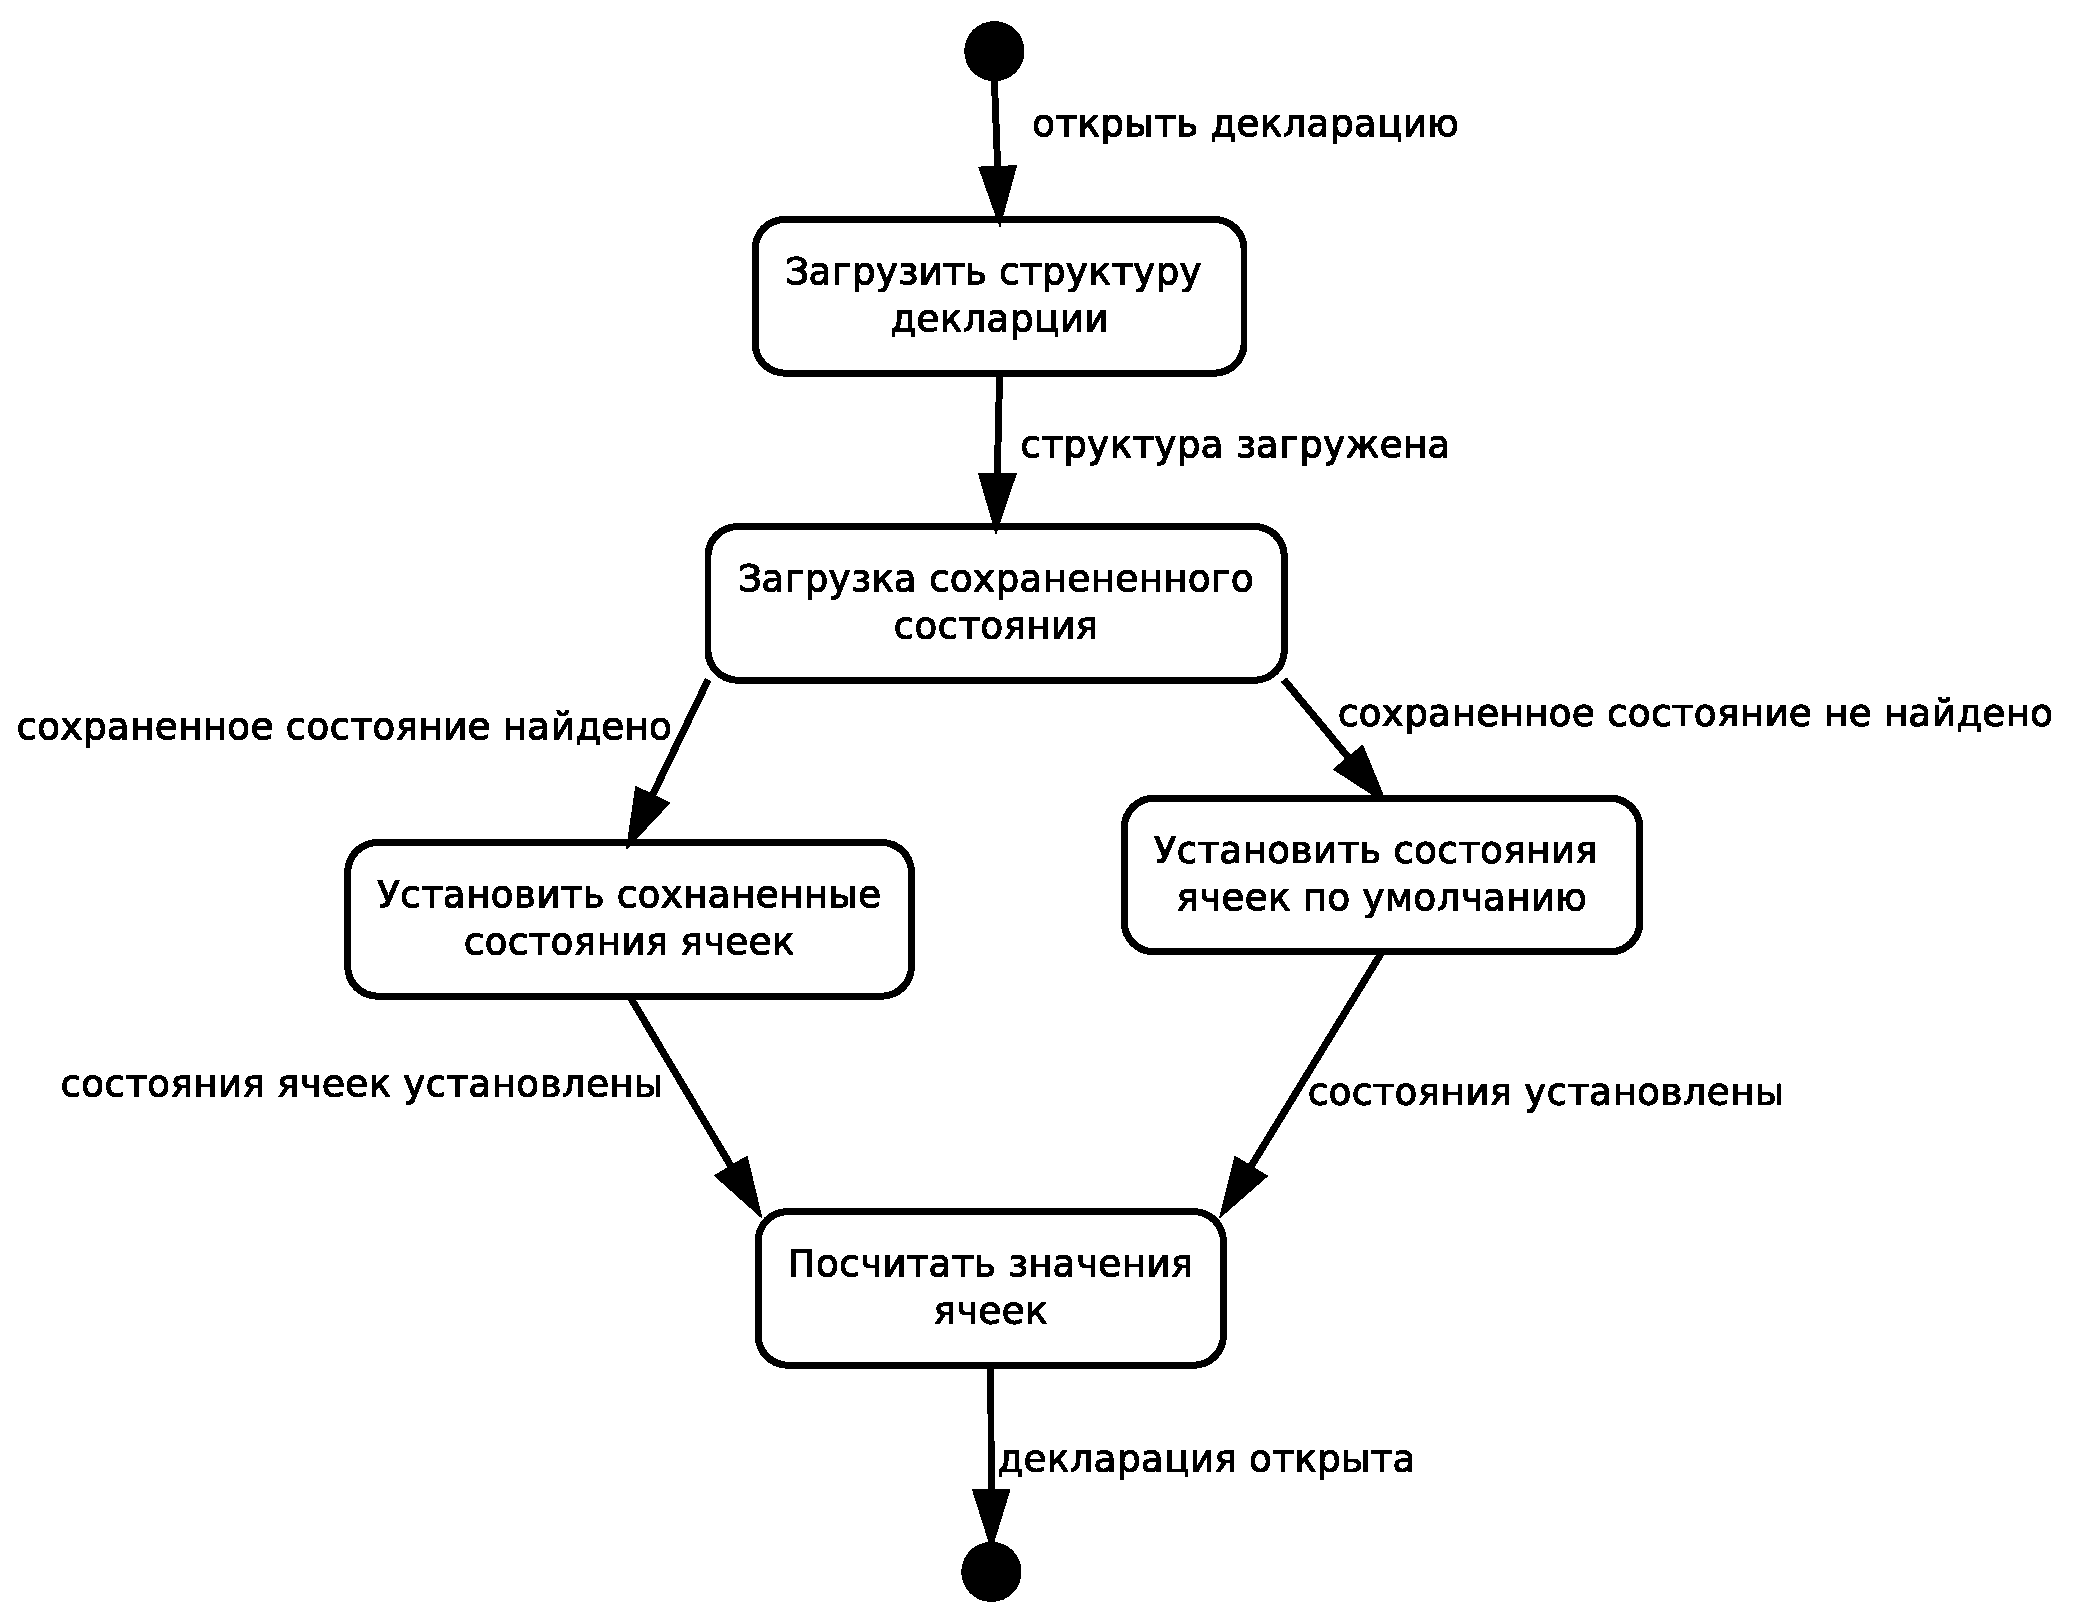
\includegraphics[scale=0.4]{uml/states_1}
  \caption{Диаграмма состояний для открытия деклараций}
  \label{pic:states_1}
\end{figure}

\subsection{Создание прототипа пользовательского интерфейса}

Процесс коммуникации системы с пользователем будет осуществляться посредством графического пользовательского интерфейса. На основании вариантов использования создадим прототип пользовательского интерфейса, рассмотрим каждый вариант использования.

На диаграмме вариантов использования для работы с компанией пользователю необходимо осуществлять создание, редактирования и удаление сущности <<Компания>>. Создание и редактирование объекта может осуществляться посредством формы, на которой содержатся элементы ввода для параметров <<Компании>>.
%todo:привести пример формы
Для удаления и редактирования компании, пользователю необходимо осуществить выбор компании, которую он хотел бы редактировать или изменить. Для этих целей можно предоставить пользователю список, на котором будут изображены все созданные компании, с элементами управления, по нажатию на которые будет отображена форма редактирования, либо объект будет удален.
%todo:привести пример списка

Рассмотрим варианты использования для работы с бухгалтерской книгой. Для создания и редактирования <<Бухгалтерской книги>> необходимо предоставить пользователю форму, на которой будут располагаться элементы ввода для параметров бухгалтерской книги( <<Компания>> которой она будет принадлежать, <<название>>). Для возможности добавления и редактирования <<Счетов>> бухгалтерской книги необходимо предоставить элементы, по нажатию на которые будет осуществлено добавление либо удаление <<Счета>>. Для работы со <<Счетом>> необходимо предоставить панель, которая будет содержать элементы ввода для параметров <<Счета>> (<<номер>>, <<кредит>>, <<дебет>>). При добавлении счета на форме будет добавляться панель, при удалении счета, соответствующая ему панель будет удаляться.
%todo:привести пример формы бухгалтерской книги
Для возможности выбора пользователем бухгалтерской книги, которую он хотел бы удалить или отредактировать, необходимо использовать список, на котором будут отображаться созданные бухгалтерские книги.
%todo:привести пример списка бухгалтерской книги

Рассмотрим варианты использования для работы с налоговыми формами. Создания и редактирование <<Налоговыми формами>> будет осуществляться посредством формы на которой будут содержаться элементы выбора и ввода параметров объекта. Нужно учесть тот факт, что пользователю нужно выбрать <<Компанию>>, затем для выбранной компании выбрать <<Бухгалтерскую книгу>>.
%todo:привести пример формы создания редактирования налоговых форм
Для возможности выбора пользователем налоговых форм, которые он хотел бы отредактировать либо удалить, необходимо использовать список, на котором будут отображаться созданные налоговые формы, напротив каждой налоговой формы следует расположить элементы, по нажатию на которые будет отображена форма редактирования, либо удалена соответствующая налоговая форма. Так же для того что бы работать с декларациями, в списке напротив каждого объекта расположим элемент, состояние которого будет показывать выбран ли он в качестве активного. Пользователь будет работать именно с декларациями активных налоговых форм.
%todo:привести пример списка налоговых форм

Далее рассмотрим варианты использования для работы с декларацией. Для выбора декларации, которую необходимо открыть пользователю будет использоваться список доступных деклараций. Форма декларации должна содержать ячейки, которые будут представлять собой элементы ввода, в зависимости от типа ячейки они будут доступны, либо не доступны для редактирования (пользовательский тип ячейки будет доступна для редактирования, так как значение должен ввести пользователь). При выборе пользователем конкретной ячейки необходимо отобразить панель, которая будет содержать текущие параметры ячейки, в зависимости от типа ячейки будут содержаться элементы ввода для изменения параметров.
%todo:привести пример списка деклараций.
%todo:привести пример декларации.

\section{Детализация объектов}
Рассмотрим объекты системы на более низком уровне абстракции.

На рисунке~\ref{pic:classes_1} изобразим основные объекты системы. Был введен новый объект <<СостояниеДекларации>>, являющийся представлением экземпляра декларации для <<НалоговыхФорм>>. Данный объект имеет атрибут <<состоянияЯчеек>>, который представляет собой список состояний всех ячеек декларации. Объект <<СостояниеЯчейки>> содержит атрибут <<типыЯчеек>>, который представляет собой список <<ТиповЯчейки>>, список содержит возможные типы, которые может представлять ячейка. Объект <<Значение>> содержит значение ячейки, объект был введен так как типы данных значений ячеек могут быть разными.

\begin{sidewaysfigure}
  \centering
  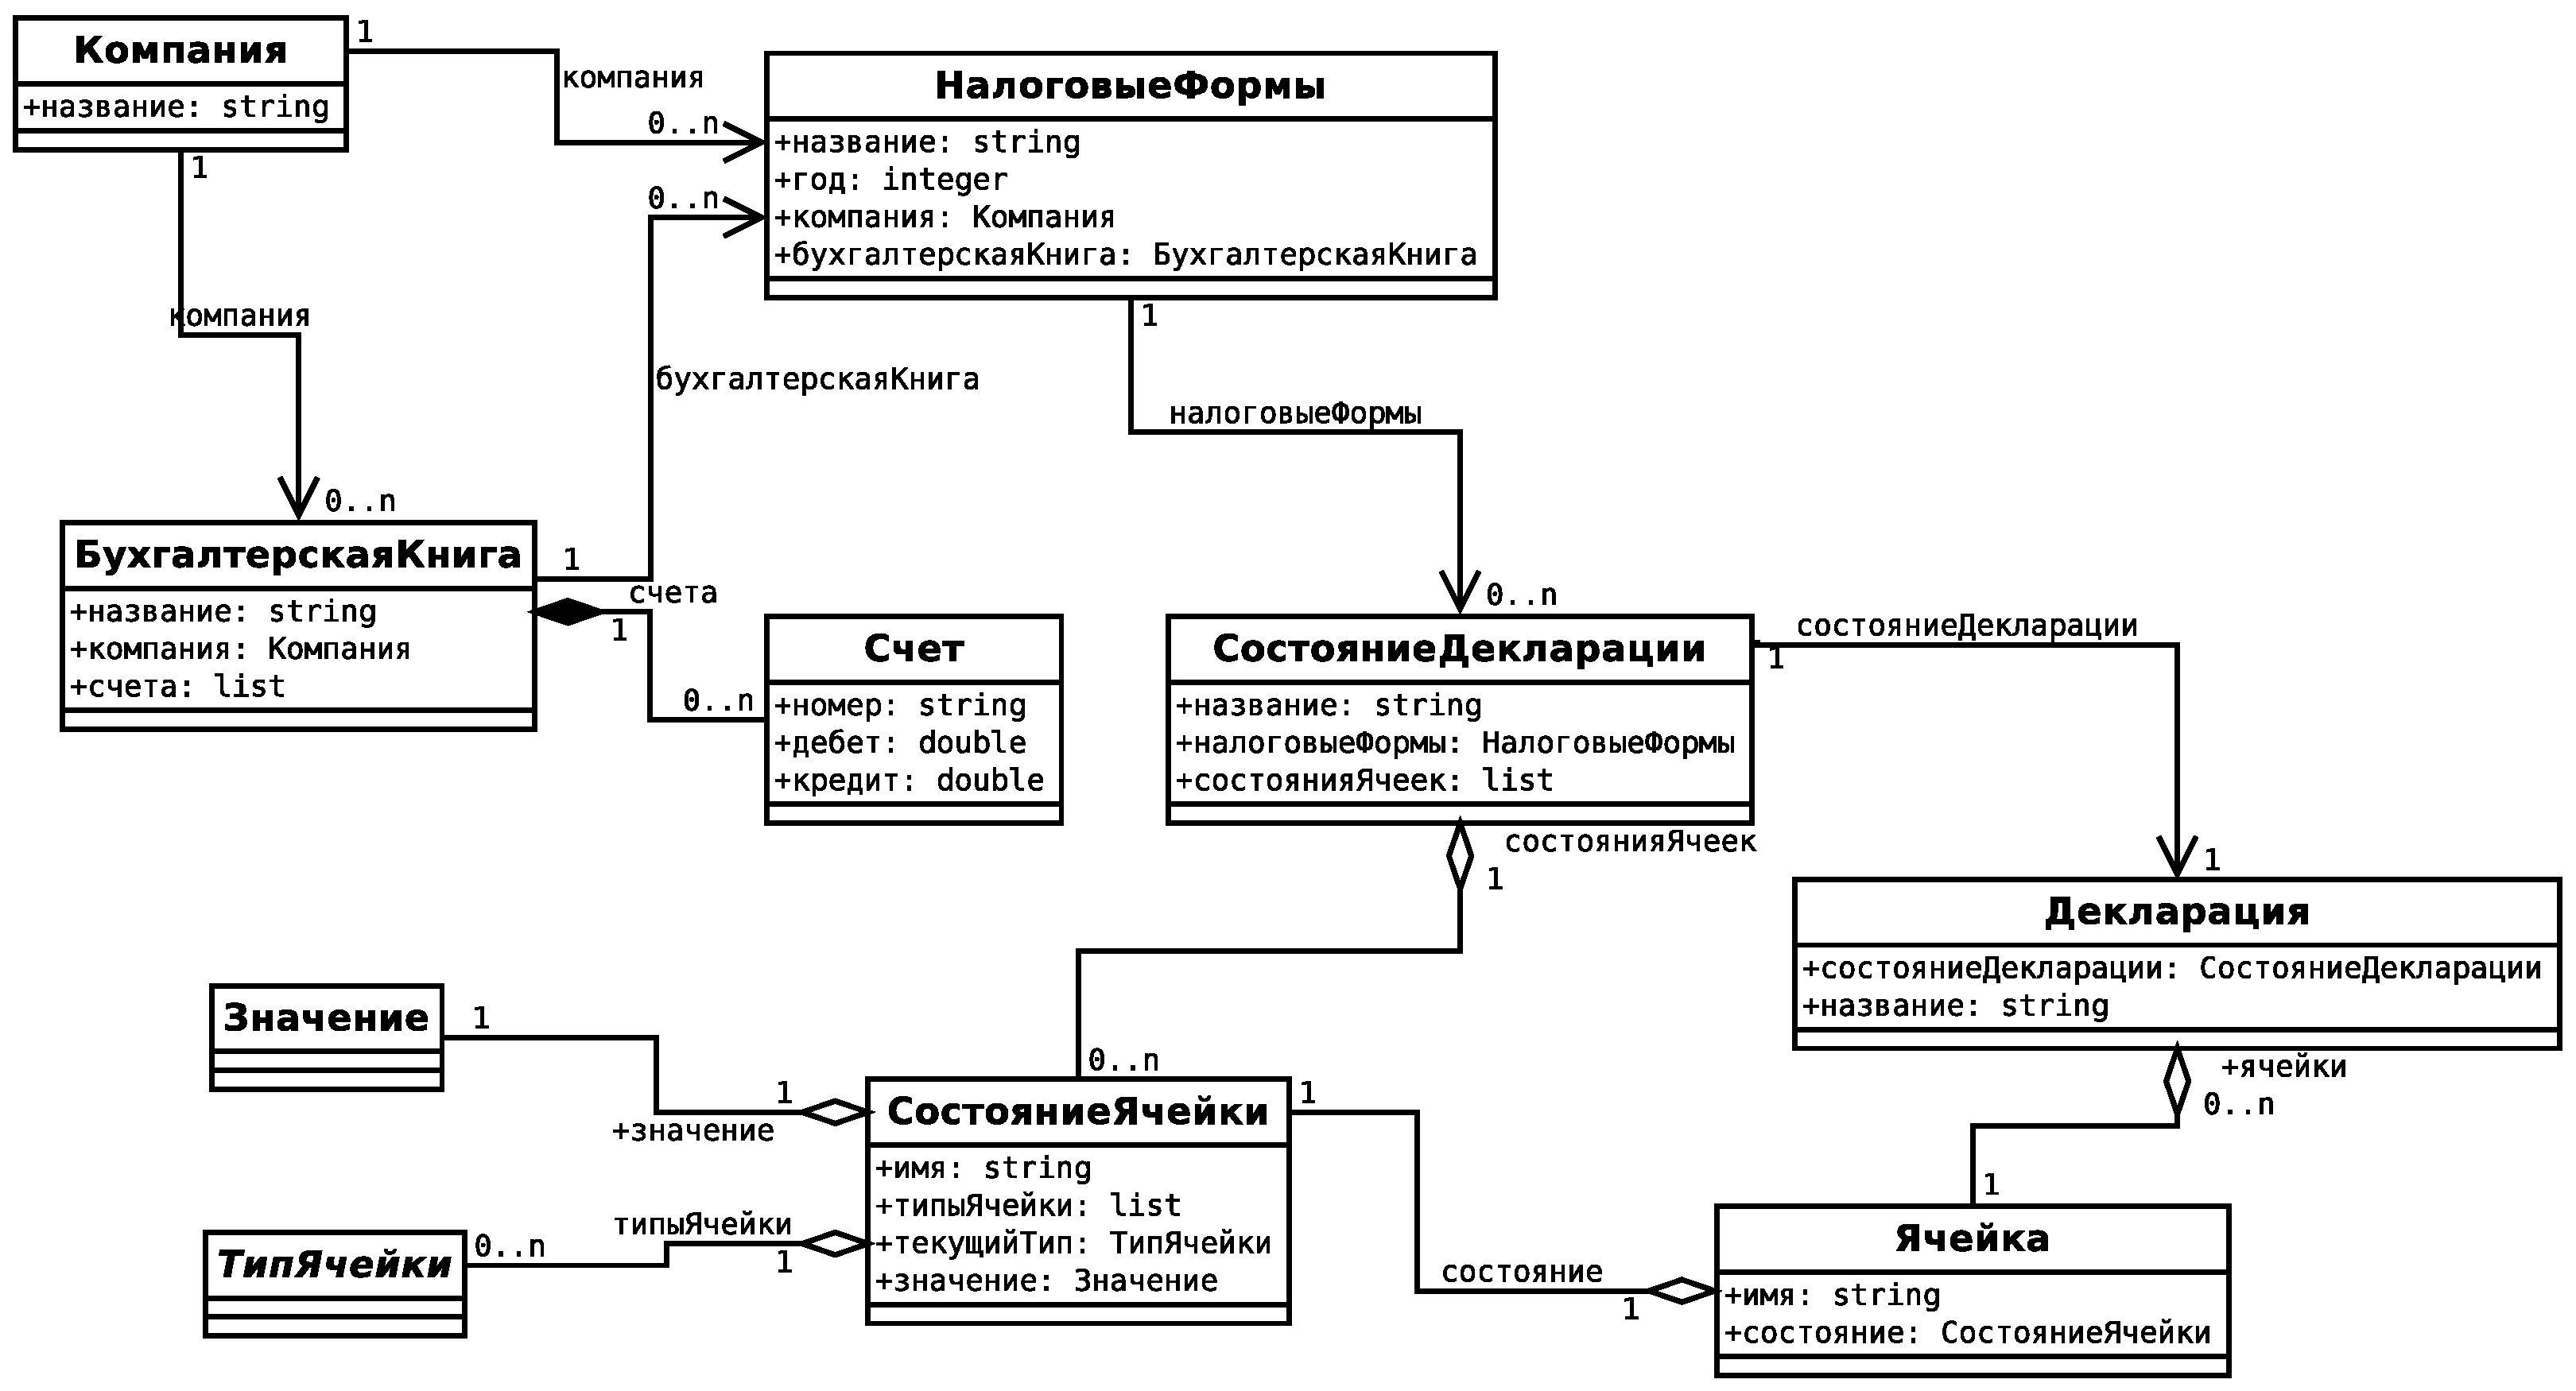
\includegraphics[scale=0.4]{uml/_classes_1}
  \caption{Диаграмма основных объектов системы}
  \label{pic:classes_1}
\end{sidewaysfigure}

Рассмотрим диаграмму, на которой приведены объекты, участвующие в подсчете декларации. <<КалькуляторДекларации>> содержит метод <<посчитатьДекларацию>>, который подсчитывает значения ячеек декларации и устанавливает значения для ячеек. Метод <<пересчитатьЯчейку>> пересчитывает одну ячейку и возвращает список пересчитанных ячеек (включая данную), которые являются зависимыми от данной (например, если значение какой-либо формулы зависит от значения пересчитываемой ячейки, то при пересчете должна пересчитаться и формула). Объект <<Контекст>>  содержит значения уже посчитанных ячеек, значение можно установить вызовом метода <<установитьЗначение>>, для получения значения используется метод <<получитьЗначение>>. Для подсчета значения каждой ячейки используется объект <<КалькуляторЯчейки>>, данный объект содержит абстрактный метод <<посчитать>>, который принимает в качестве параметров <<ТипЯчеки>> и <<Контекст>>.

\begin{figure}
  \centering
  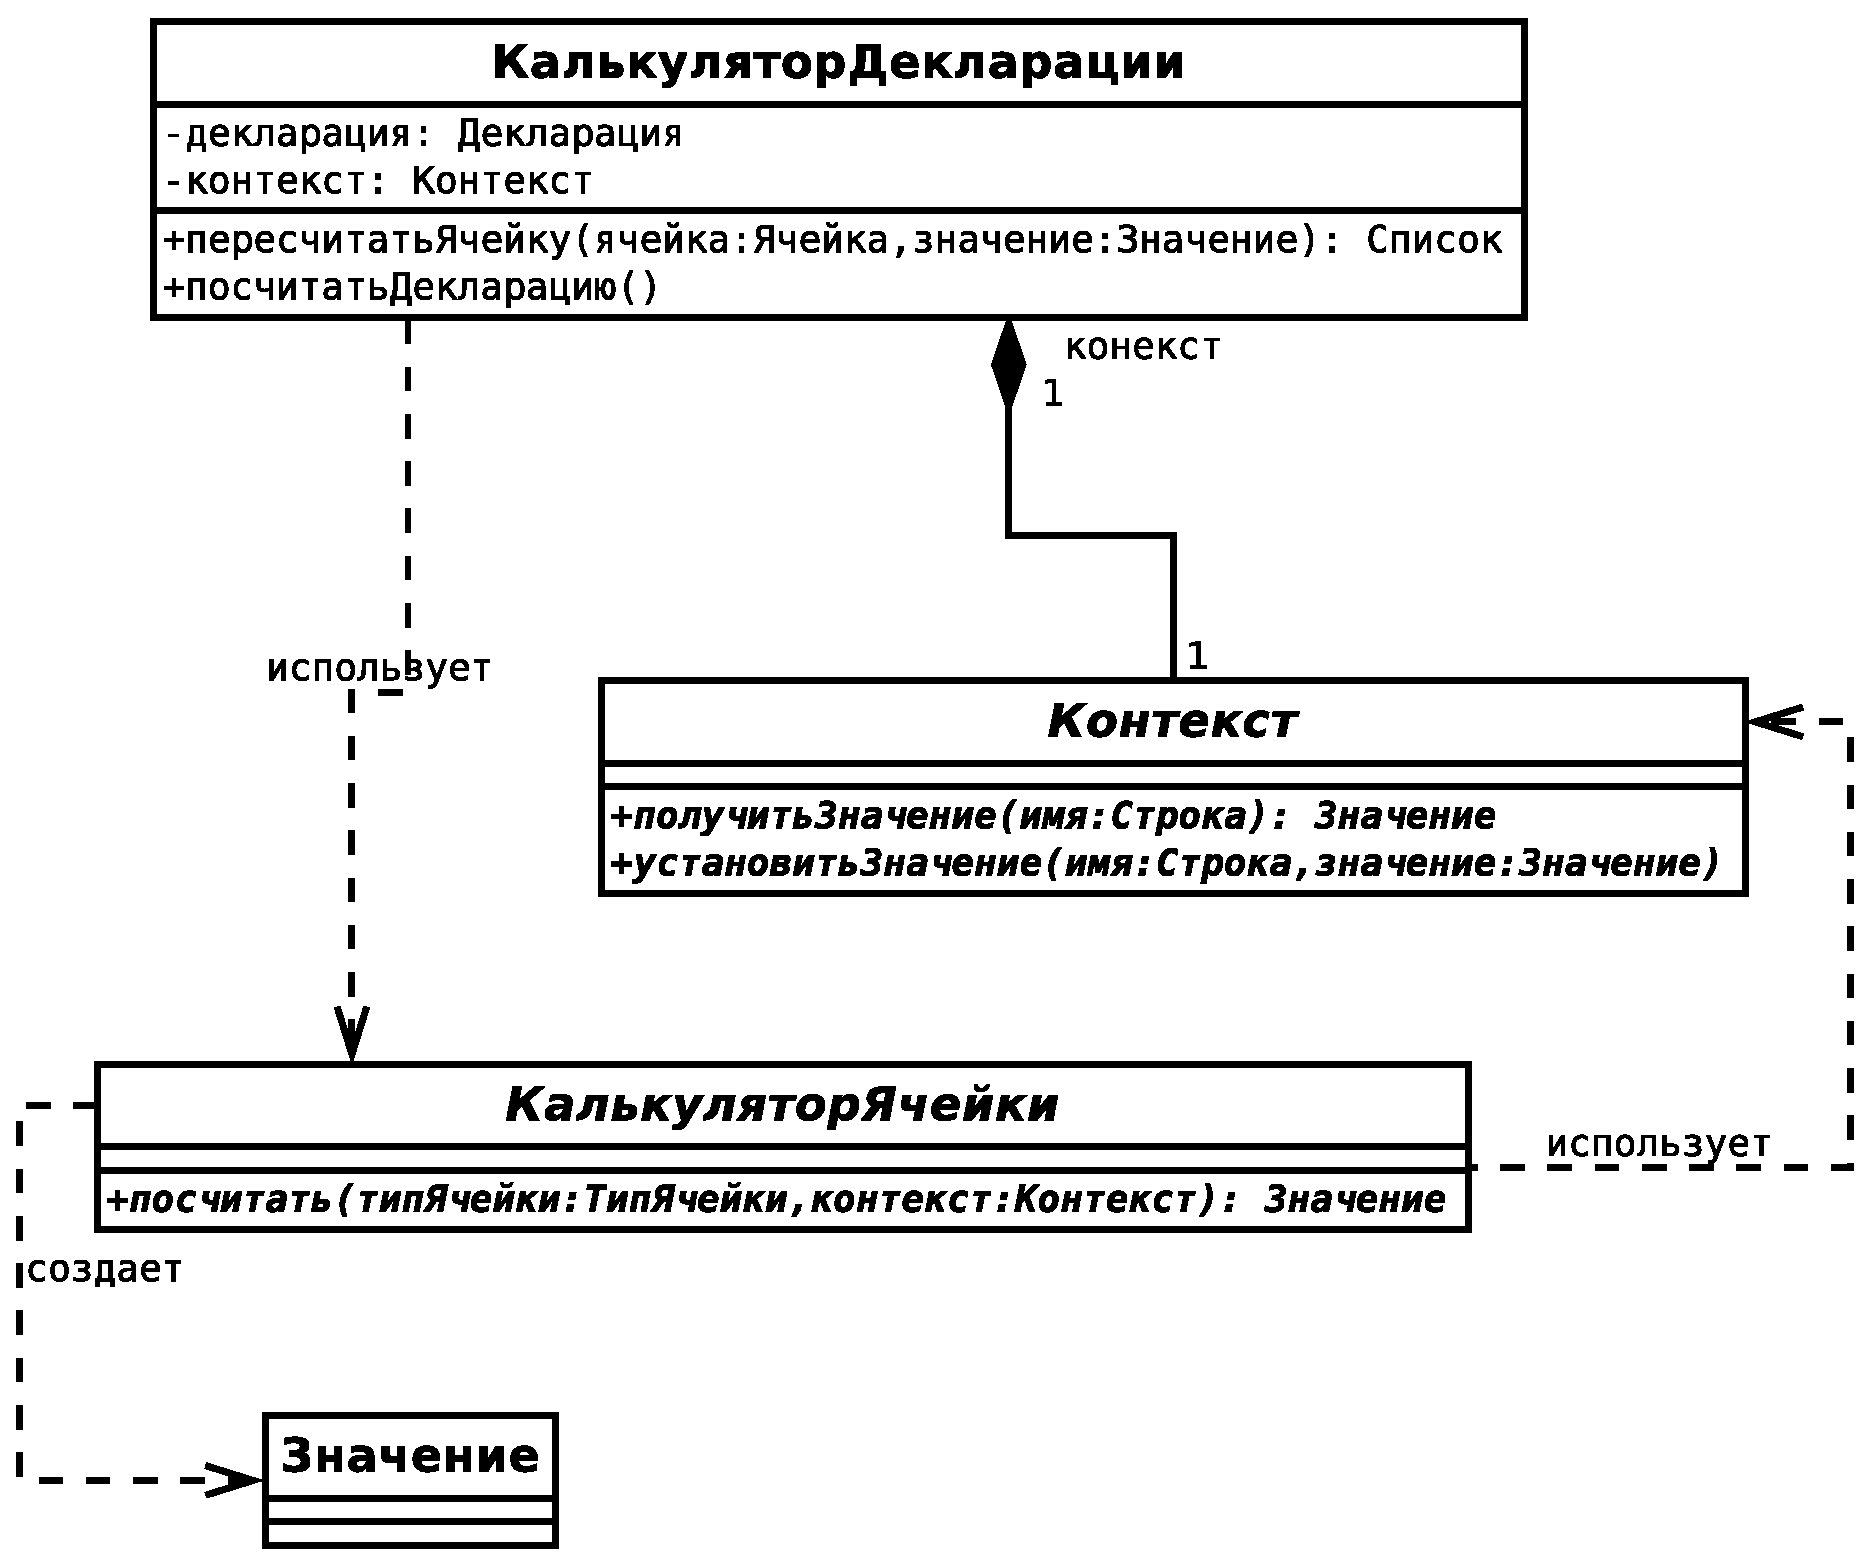
\includegraphics[scale=0.4]{uml/_classes_3}
  \caption{Диаграмма объектов, участвующих в подсчете декларации}
  \label{pic:classes_3}
\end{figure}

Подробнее рассмотрим объекты, участвующие в подсчете ячейки (рисунок \ref{pic:classes_2}). Объекты <<Пользовательская>>, <<Счета>> и <<Формула>> расширяют объект <<ТипЯчейки>>, представляя соответственно пользовательский, счета и формульный тип ячеек. Тип <<Счета>> содержит атрибут <<интервалы>>, который представляет собой список интервалов для подсчета ячейки. Объект <<КалькуляторСчетовойЯчейки>>, <<КалькуляторФормульнойЯчейки>> и <<КалькуляторПользовательскойЯчейки>> реализуют абстрактный метод <<посчитать>> объекта <<КалькуляторЯчейки>> для подсчета ячеек разных типов (счета, формульная и пользовательская). <<КалькуляторСчетовойЯчейки>> использует <<БухгалтерскуюКнигу>> для подсчета ячейки, так как подсчет интервалов использует <<Счета>>, лежащие в данном интервале. На рисунке~\ref{pic:algo_accounts} приведен алгоритм подсчета счетовой ячейки.

\begin{figure}
  \centering
  \includegraphics[scale=0.4]{uml/algo_accounts_calc}
  \caption{Алгоритм подсчета ячейки типа <<Счета>>}
  \label{pic:algo_accounts}
\end{figure}

\begin{sidewaysfigure}
  \centering
  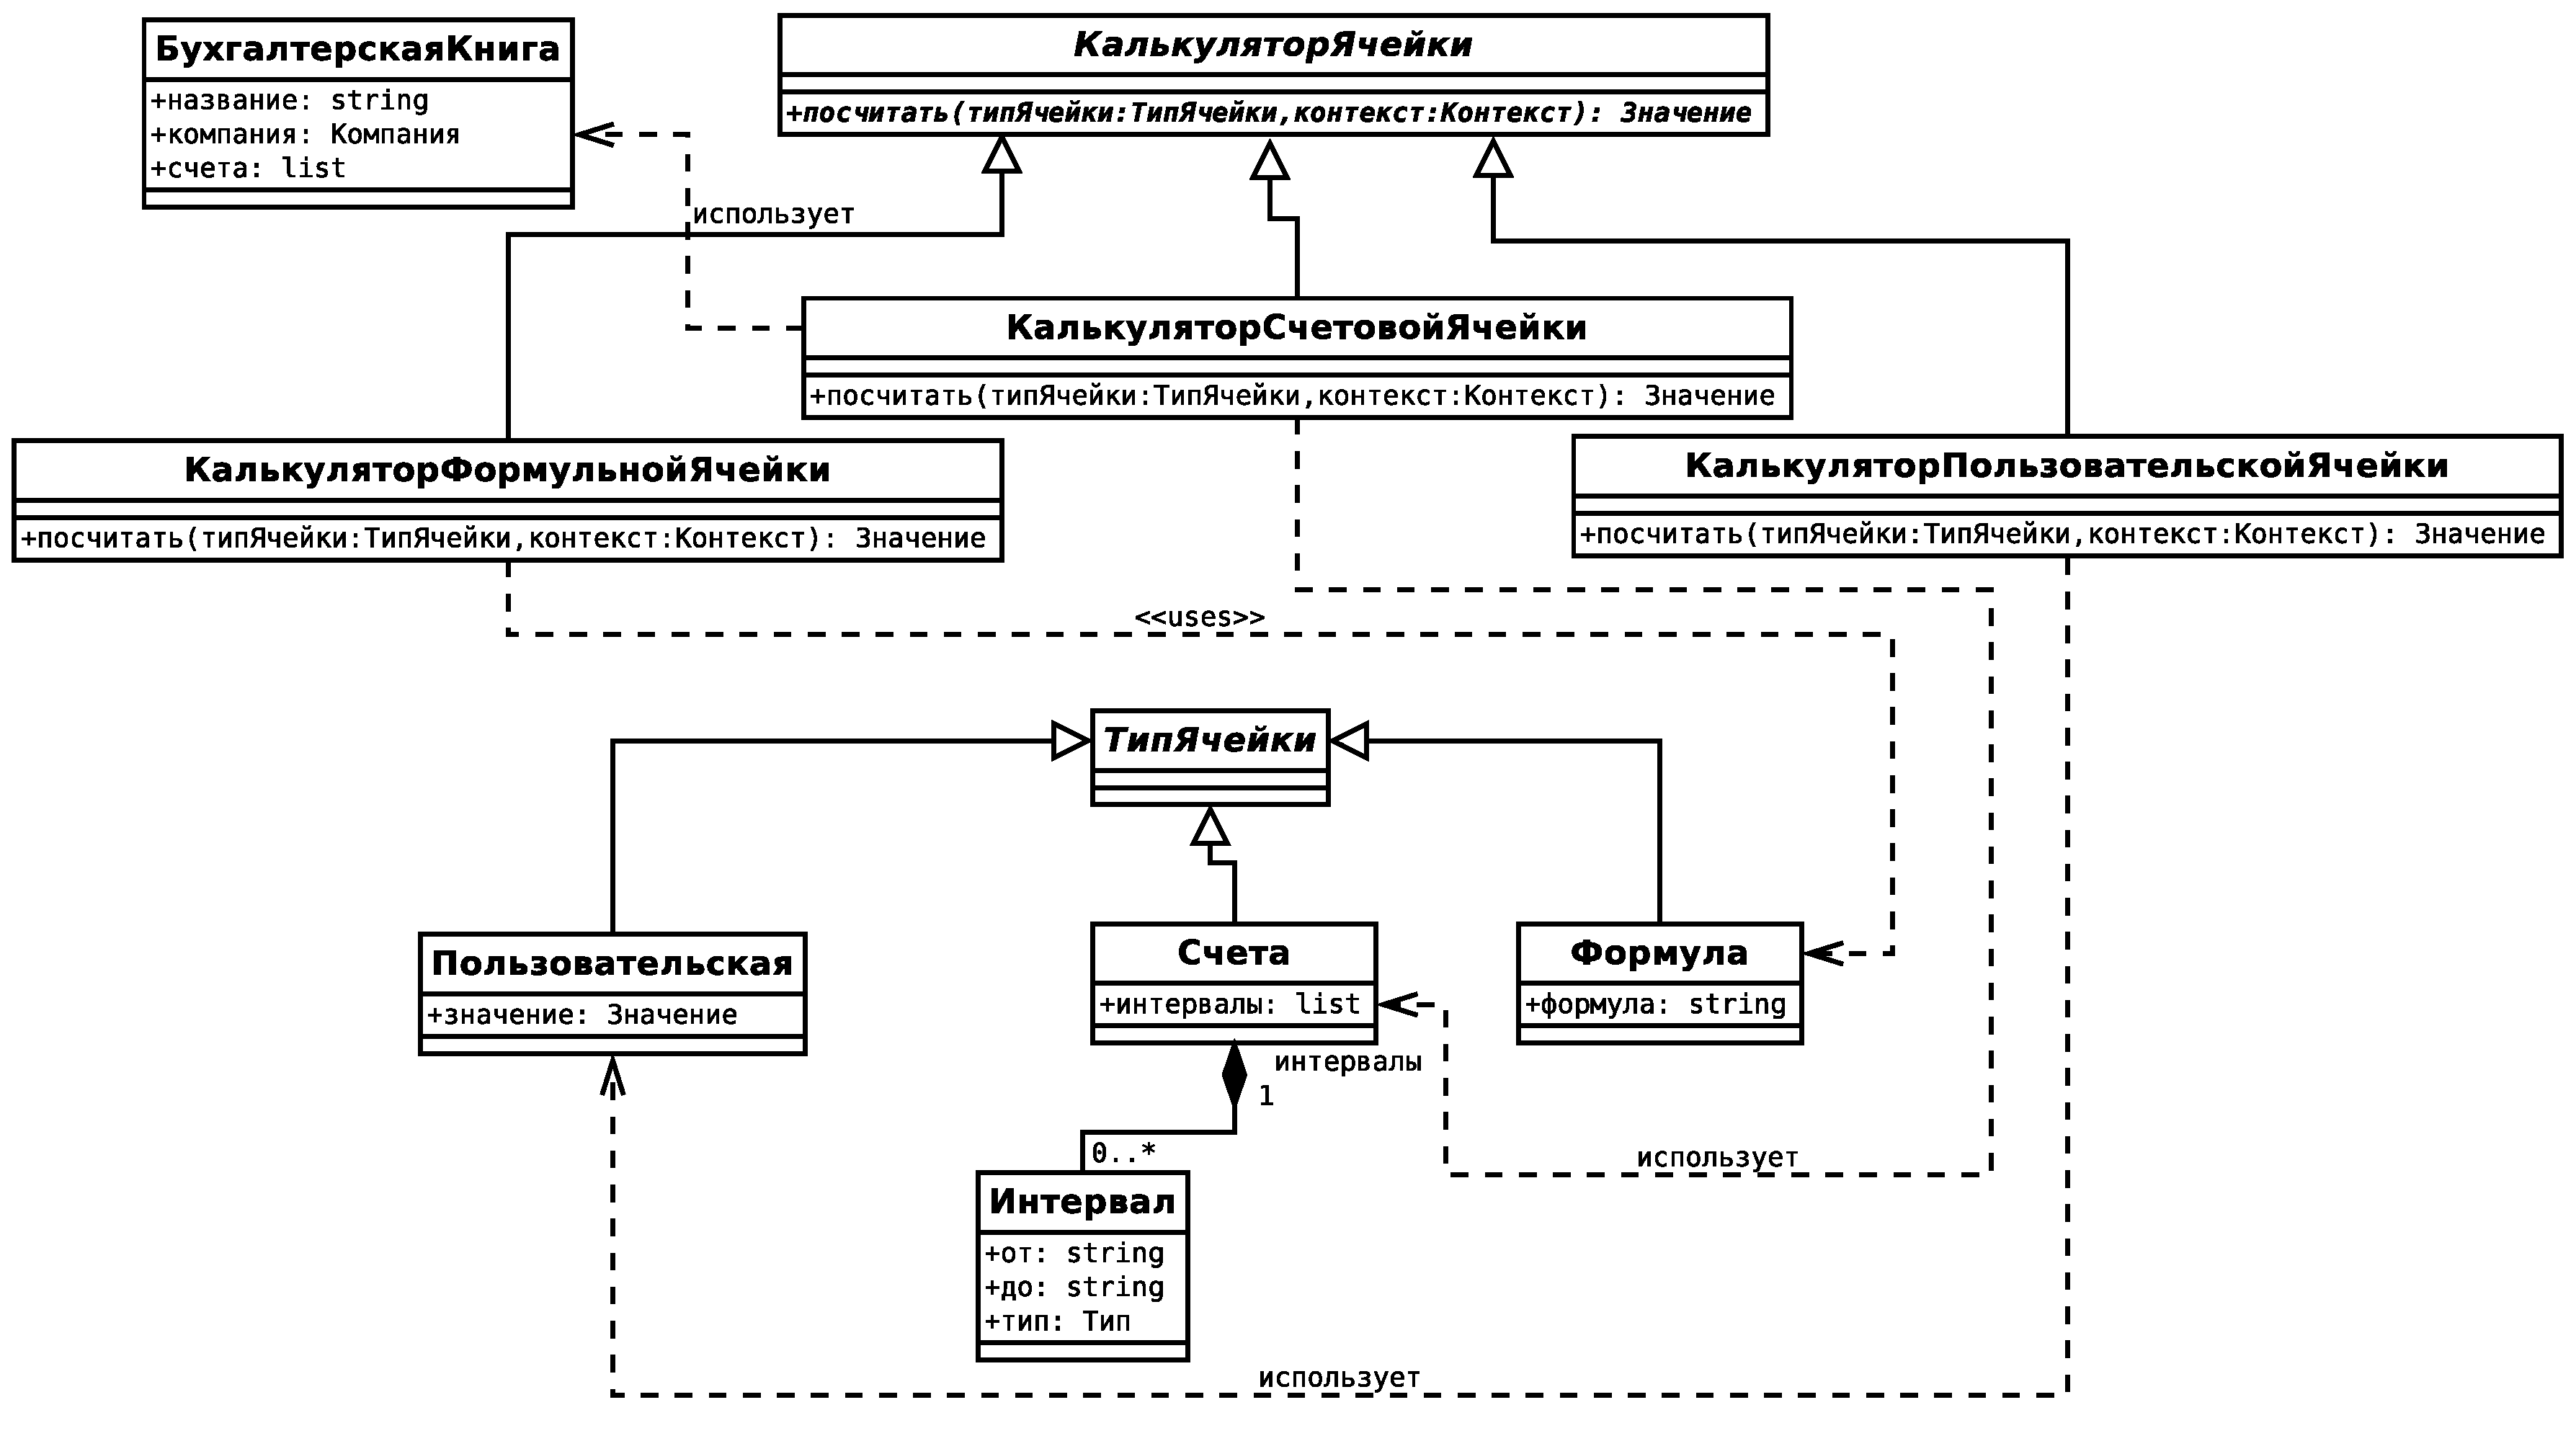
\includegraphics[scale=0.4]{uml/_classes_2}
  \caption{Диаграмма объектов, участвующих в подсчете ячейки}
  \label{pic:classes_2}
\end{sidewaysfigure}

Рассмотрим процесс вычисления значения формульных ячеек. Для подсчета данного типа ячеек требуется вычислить значение математического выражения, заданного на формальном языке.

На рисунке~\ref{pic:evalprocess} представлен алгоритм вычисления значения выражения. Первым этапом является лексический анализ -- процесс аналитического разбора входной последовательности символов  с целью получения на выходе последовательности символов, называемых токенами. Токен -- последовательность символов, соответствующая лексеме. То есть в процессе лексического анализа производится распознавание и выделение лексем из входной последовательности символов. Следующим этапом является синтаксический анализ --  это процесс сопоставления линейной последовательности лексем языка с его формальной грамматикой. Результатом является АСД -- конечное, помеченное, ориентированное дерево, в котором внутренние вершины сопоставлены с операторами языка, а листья с соответствующими операндами. Таким образом листья являются пустыми операторами и представляют только переменные и константы. Следующим этапом является интерпретация -- анализ полученного АСД с целью вычисления значения выражения.

\begin{figure}[ht]
  \centering
  \includegraphics[scale=0.4]{uml/eval_algorithm}
  \caption{Процесс вычисления значения выражения}
  \label{pic:evalprocess}
\end{figure}

Опишем лексемы, которые присутствуют в данном языке выражений. Идентификаторы представляют собой последовательность букв латинского алфавита, цифр от 0 до 9, символа подчеркивания(<<\_>>), но не могут начинаться с цифры. Идентификаторы используются для названия функций. Переменные представляют собой последовательность символов, которая может содержать буквы, цифры, знак подчеркивания, заключенную между <<\$\{<< слева и <<\}>> справа. Строковые константы представляют собой набор символов, заключенных между ', они могут содержать любые символы, за исключением ', который должен быть представлен последовательностью \textbackslash . Целочисленные константы записываются последовательностью цифр от 0 до 9, опциональным является использование знака <<->> вначале. Вещественные числа записываются с десятичной частью (разделитель <<.>>), с необязательной десятичной экспонентой, примеры записи десятичных чисел: 3.0, 3.1416, 314.16e-2, 0.31416E1.

Язык содержит стандартные арифметические операторы: бинарные +(сложение), -(вычитание), *(умножение), /(деление), \textasciicircum (возведение в степень), унарный -(отрицательное значение). Операциями сравнения являются: ==(операция сравнения), !=(операция <<не равно>>), <(меньше), >(больше), <=(<<не больше>>), >=(<<не меньше>>). Логические операции: <<\&\&>> (логическое <<и>>), <<||>> (логическое <<или>>), <<!>> (отрицание).

Было выделено четыре типа данных которые содержит язык: строковое, целое, вещественное, булево (true или false).

Опишем синтаксис языка с использованием расширенной формой Бэкуса-Наура \cite{refebnf}. Расширенная форма Бэкуса-Наура -- формальная система определения синтаксиса, в которой одни синаксические категории определяются через другие. Синтаксис:

\begin{lstlisting}[language=Python,basicstyle=\small,morekeywords={number,integer,double,simple\_expr, func\_call,unary\_op, expression, params, variable, str\_const, bin\_op, ident},keywordstyle=\it]
 number = integer | double
 simple_expr = number | str_const | variable
          | func_call | '(',expression,')'
 unary_op = '-' | '!'
 bin_op = '<' | '>' | '<=' | '>='
          | '+' | "-" | '*' | '/' | '&'
          | '&&' | '||' | '^'
 expression = simple_expr | unary_op expression
          | {bin_op, expression }
 func_call = ident, '(',  ')' | ident, '(', params, ')'
 params = expression | expression ',' params
\end{lstlisting}

Приведем объекты, которые будут участвовать в подсчете значения выражения (рисунок~\ref{pic:classes_4}).
Объект <<ЛексическийАнализатор>> выполняет лексический анализ выражения, которое представлено атрибутом <<выражение>> строкового типа. <<СинтаксическийАнализатор>> производит анализ лексем, которые получаются с использованием <<ЛексическогоАнализатора>>, результатом анализа является АСД, которое используется объектом <<ОценщикВыражения>> для вычисления результата выражения.

\begin{figure}
  \centering
  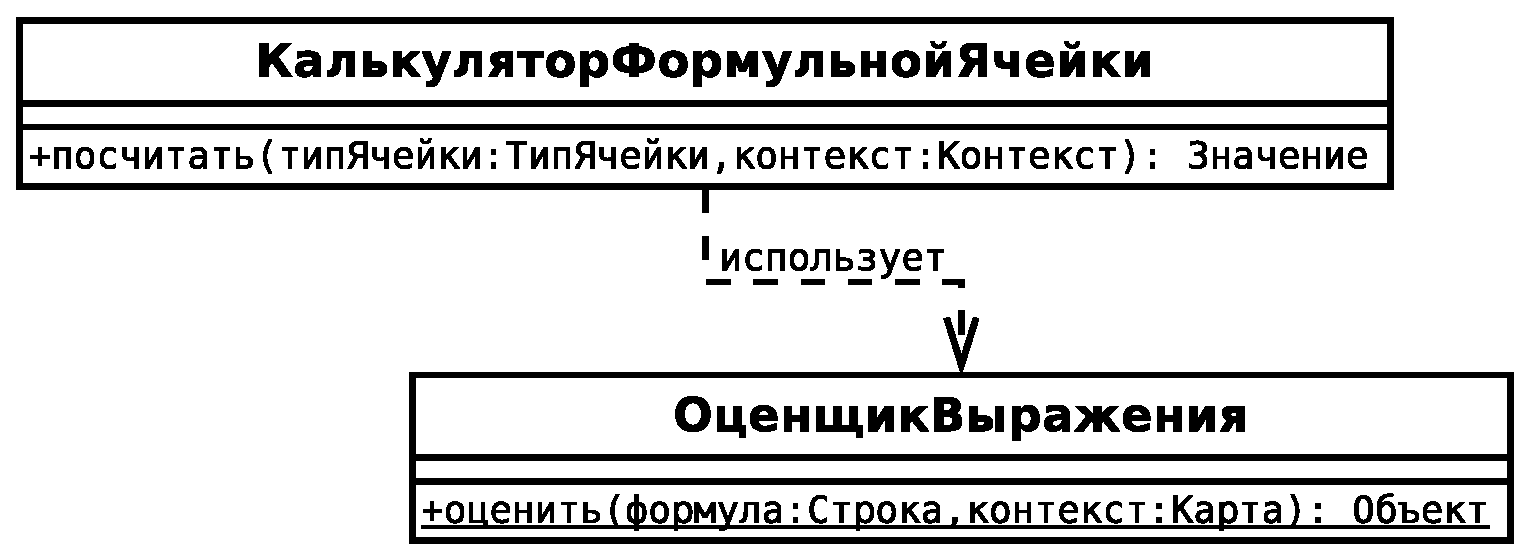
\includegraphics[scale=0.5]{uml/_classes_4}
  \caption{Диаграмма объектов, участвующих в подсчете выражения}
  \label{pic:classes_4}
\end{figure}

\section{Представление декларации в формате XML}
Для хранения структуры декларации был выбран язык XML\cite{xmlbas}. XML — это иерархическая структура, предназначенная для хранения любых данных. Визуально структура может быть представлена как дерево. Важнейшее обязательное синтаксическое требование заключается в том, что документ имеет только один корневой элемент. Это означает, что текст или другие данные всего документа должны быть расположены между единственным начальным корневым тегом и соответствующим ему конечным тегом.

Для описания структуры декларации необходимо описать свойства объектов: <<Декларация>>, <<Ячейка>>, свойство <<ТипыЯчеек>> (что является списком, который содержит объекты типа <<ТипЯчейки>>) объекта <<СостояниеЯчейки>>. Свойства <<Декларации>> возможно выделить в иерархическую структуру (рисунок~\ref{pic:xmlrepresentation}).

\begin{figure}[ht]
  \centering
  \includegraphics[scale=0.5]{uml/xmlrepresentation}
  \caption{Структура XML документа, представляющего структуру декларации}
  \label{pic:xmlrepresentation}
\end{figure}

\section{Логическая модель базы данных}
Представим логическую модель базы данных (рисунок~\ref{pic:domain_model}). На диаграмме отображены объекты, которые будут храниться в базе данных и отношения между ними. Объект <<Компания>> может иметь <<НалоговыеФормы>> и <<БухлалтерскиеКниги>>. <<БухгалтерскаяКнига>> может содержать <<Счета>>. <<НалоговыеФормы>> могут содержать <<СостоянияДекларации>>. <<СостояниеДекларации>> сожержит <<СостояниеЯчеек>>. Объект <<СостояниеЯчейки>> содержит <<Значение>> и текущий <<ТипЯчейки>>. <<ТипЯчейки>> может быть <<Счета>>, <<Пользовательская>> и <<Формула>> (на диаграмме данное отношение изображено как наследование). Тип ячейки <<Счета>> содержит <<Интервалы>>.\\

\begin{figure}[ht]
  \centering
  \includegraphics[scale=0.37]{uml/domainmodel}
  \caption{Логическая модель данных}
  \label{pic:domain_model}
\end{figure}

\chapter{Реализация системы учета и управления электронными налоговыми декларациями}

\section{Выбор и обоснование средств разработки}
Для реализации системы документооборота использовался язык программирования Java. Java --- объектно-ориентированный язык программирования, разрабатываемый компанией Sun Microsystems.Программы на Java транслируются в байт-код, выполняемый виртуальной машиной Java (JVM) --- программой, обрабатывающей байтовый код и передающей инструкции оборудованию как интерпретатор, но с тем отличием, что байтовый код, в отличие от текста, обрабатывается значительно быстрее.


Достоинство подобного способа выполнения программ --- в полной независимости байт-кода от операционной системы и оборудования, что позволяет выполнять Java-приложения на любом устройстве, для которого существует соответствующая виртуальная машина. Другой важной особенностью технологии Java является гибкая система безопасности благодаря тому, что исполнение программы полностью контролируется виртуальной машиной. Любые операции, которые превышают установленные полномочия программы (например, попытка несанкционированного доступа к данным или соединения с другим компьютером) вызывают немедленное прерывание.


Особенности языка:
\begin{gostitemize}
  \gostitem{автоматическое управление памятью;}
  \gostitem{расширенные возможности обработки исключительных ситуаций;}
  \gostitem{богатый набор средств фильтрации ввода/вывода;}
  \gostitem{набор стандартных коллекций, таких как массив, список, стек;}
  \gostitem{наличие простых средств создания сетевых приложений;}
  \gostitem{наличие классов, позволяющих выполнять HTTP-запросы и обрабатывать ответы;}
  \gostitem{встроенные в язык средства создания много-поточных приложений.}
\end{gostitemize}


Следует отметить, что для данного языка существует большое количество библиотек, распространяемых под свободными лицензиями, для работы с различными форматами файлов, работы с базами данных, для разработки пользовательских интерфейсов, написания приложений, использующих веб-интерфейс;

\section{Выбор инструментальных средств разработки}

\subsection{Фреймворк Spring}
Фреймворк Spring --- открытый фреймворк для Java-платформы. Первая версия была написана Родом Джонсоном, который впервые опубликовал её вместе с изданием своей книги <<Expert One-on-One Java EE Design and Development>>.


Фреймворк был впервые выпущен под лицензией Apache 2.0 license в июне 2003 года. Первый стабильный релиз 1.0 был выпущен в марте 2004. Последующие стабильные релизы вышли в сентябре 2004 года и марте 2005 года.


Несмотря на то, что Spring Framework не обеспечивал какую-либо конкретную модель программирования, он стал широко распространённым в Java сообществе главным образом как альтернатива и замена модели Enterprise JavaBeans. Spring Framework предоставляет большую свободу Java разработчикам в проектировании, кроме того, он предоставляет хорошо документированные и лёгкие в использовании решения проблем, возникающих при создании приложений промышленного масштаба.


Между тем, особенности ядра Spring Framework применимы в любом Java приложении, и существует множество расширений и усовершенствований для построения веб-приложений на Java Enterprise платформе. По этим причинам Spring приобрёл большую популярность и признаётся разработчиками как стратегически важный фреймворк\cite{refspringsource}.

\subsection{Библиотека Hibernate}
Библиотека Hibernate --- библиотека для языка программирования Java, предназначенная для решения задач объектно-реляционного проецирования. Она представляет собой свободное программное обеспечение с открытым исходным кодом , распространяемое на условиях GNU Lesser General Public License. Данная библиотека предоставляет лёгкий в использовании каркас (фреймворк) для отображения объектно-ориентированной модели данных в традиционные реляционные базы данных.


Целью Hibernate является освобождение разработчика от значительного объёма сравнительно низкоуровневого программирования по обеспечению хранения объектов в реляционной базе данных. Разработчик может использовать Hibernate как в процессе проектирования системы классов и таблиц <<с нуля>>, так и для работы с уже существующей базой данных.


Hibernate не только решает задачу связи классов Java с таблицами базы данных (и типов данных Java с типами данных SQL), но также предоставляет средства для автоматической генерации и обновления набора таблиц, построения запросов и обработки полученных данных и может значительно уменьшить время разработки, которое обычно тратится на ручное написание SQL- и JDBC-кода. Hibernate автоматизирует генерацию SQL-запросов и освобождает разработчика от ручной обработки результирующего набора данных и преобразования объектов, максимально облегчая перенос (портирование) приложения на любые базы данных SQL.


Hibernate обеспечивает прозрачную поддержку сохранности данных  для <<POJO>> (то есть для стандартных Java-объектов). Единственное строгое требование для сохраняемого класса --- наличие конструктора по умолчанию (без параметров).


Hibernate используется как в standalone Java-приложениях, так и в приложениях на платформе Java EE, использующих сервлеты или EJB\cite{refhibernate}.
\subsection{Сервер приложений Apache Tomcat}
Сервер приложений Tomcat --- программа-контейнер сервлетов, написанная на языке Java и реализующая спецификацию сервлетов и спецификацию JSP, которые являются стандартами для разработки веб-приложений на языке Java.


Tomcat позволяет запускать веб-приложения, содержит ряд программ для самоконфигурирования. Tomcat используется в качестве самостоятельного веб-сервера, в качестве сервера контента в сочетании с веб-сервером Apache HTTP Server, а также в качестве контейнера сервлетов в сервере приложений JBoss.

Веб-приложения, которые работают в контейнере сервлетов обычно представляют собой war-архив. Приведем структуру директорий war архива:

\begin{itemize}
  \item \textbackslash WEB-INF
    \subitem  \textbackslash classes - директория, в которой находятся скомпилированные java-классы приложения;
    \subitem  \textbackslash jsp - директория, в которой находятся jsp страницы приложения;
    \subitem  \textbackslash lib - директория, в которой находятся jar-архивы, содержащие сторонние классы, которые используются в приложении;
    \subitem  \textbackslash tld - директория, содержащая дескрипторы бибиотек тегов, которые используются на jsp страницах;
    \subitem web.xml - дескриптор веб приложения, сожержит описание и настройки сервлетов, фильтров веб приложения, может содержать описание библиотек тегов, которые используются на jsp страницах данного приложения.
\end{itemize}


\section{Программная реализация компонентов системы}

В результате выполнения проекта была разработана система учета и управления электронными налоговыми декларациями. На рисунке~\ref{pic:deployment} приведена диаграмма развертывания системы. Система представлена ввиде трех узлов: рабочая станция пользователя, сервер приложений, сервер базы данных. На сервере приложений развернута система, которая представлена двумя архивами: autotax.war и autotax-engine.jar. Архив autotax.war представляет собой веб приложение и содержит jsp страницы и классы управления. Архив autotax-engine.jar содержит классы, которые представляют подсистему управления декларацией. Сервер базы данных предоставляет доступ к СУБД, для системы, доступ осуществляется посредством JDBC, что является платформо независимым стандартом взаимодействия приложений, написаных на java с различными СУБД. Узел рабочей станци пользователя представлен ПЭВМ, за которым находится пользователь системы. На рабочей станции пользователя должен быть запущен веб-браузер, коммуникация веб-браузера с сервером приложений осуществляется по протоколу HTTP.

\begin{figure}
  \centering
  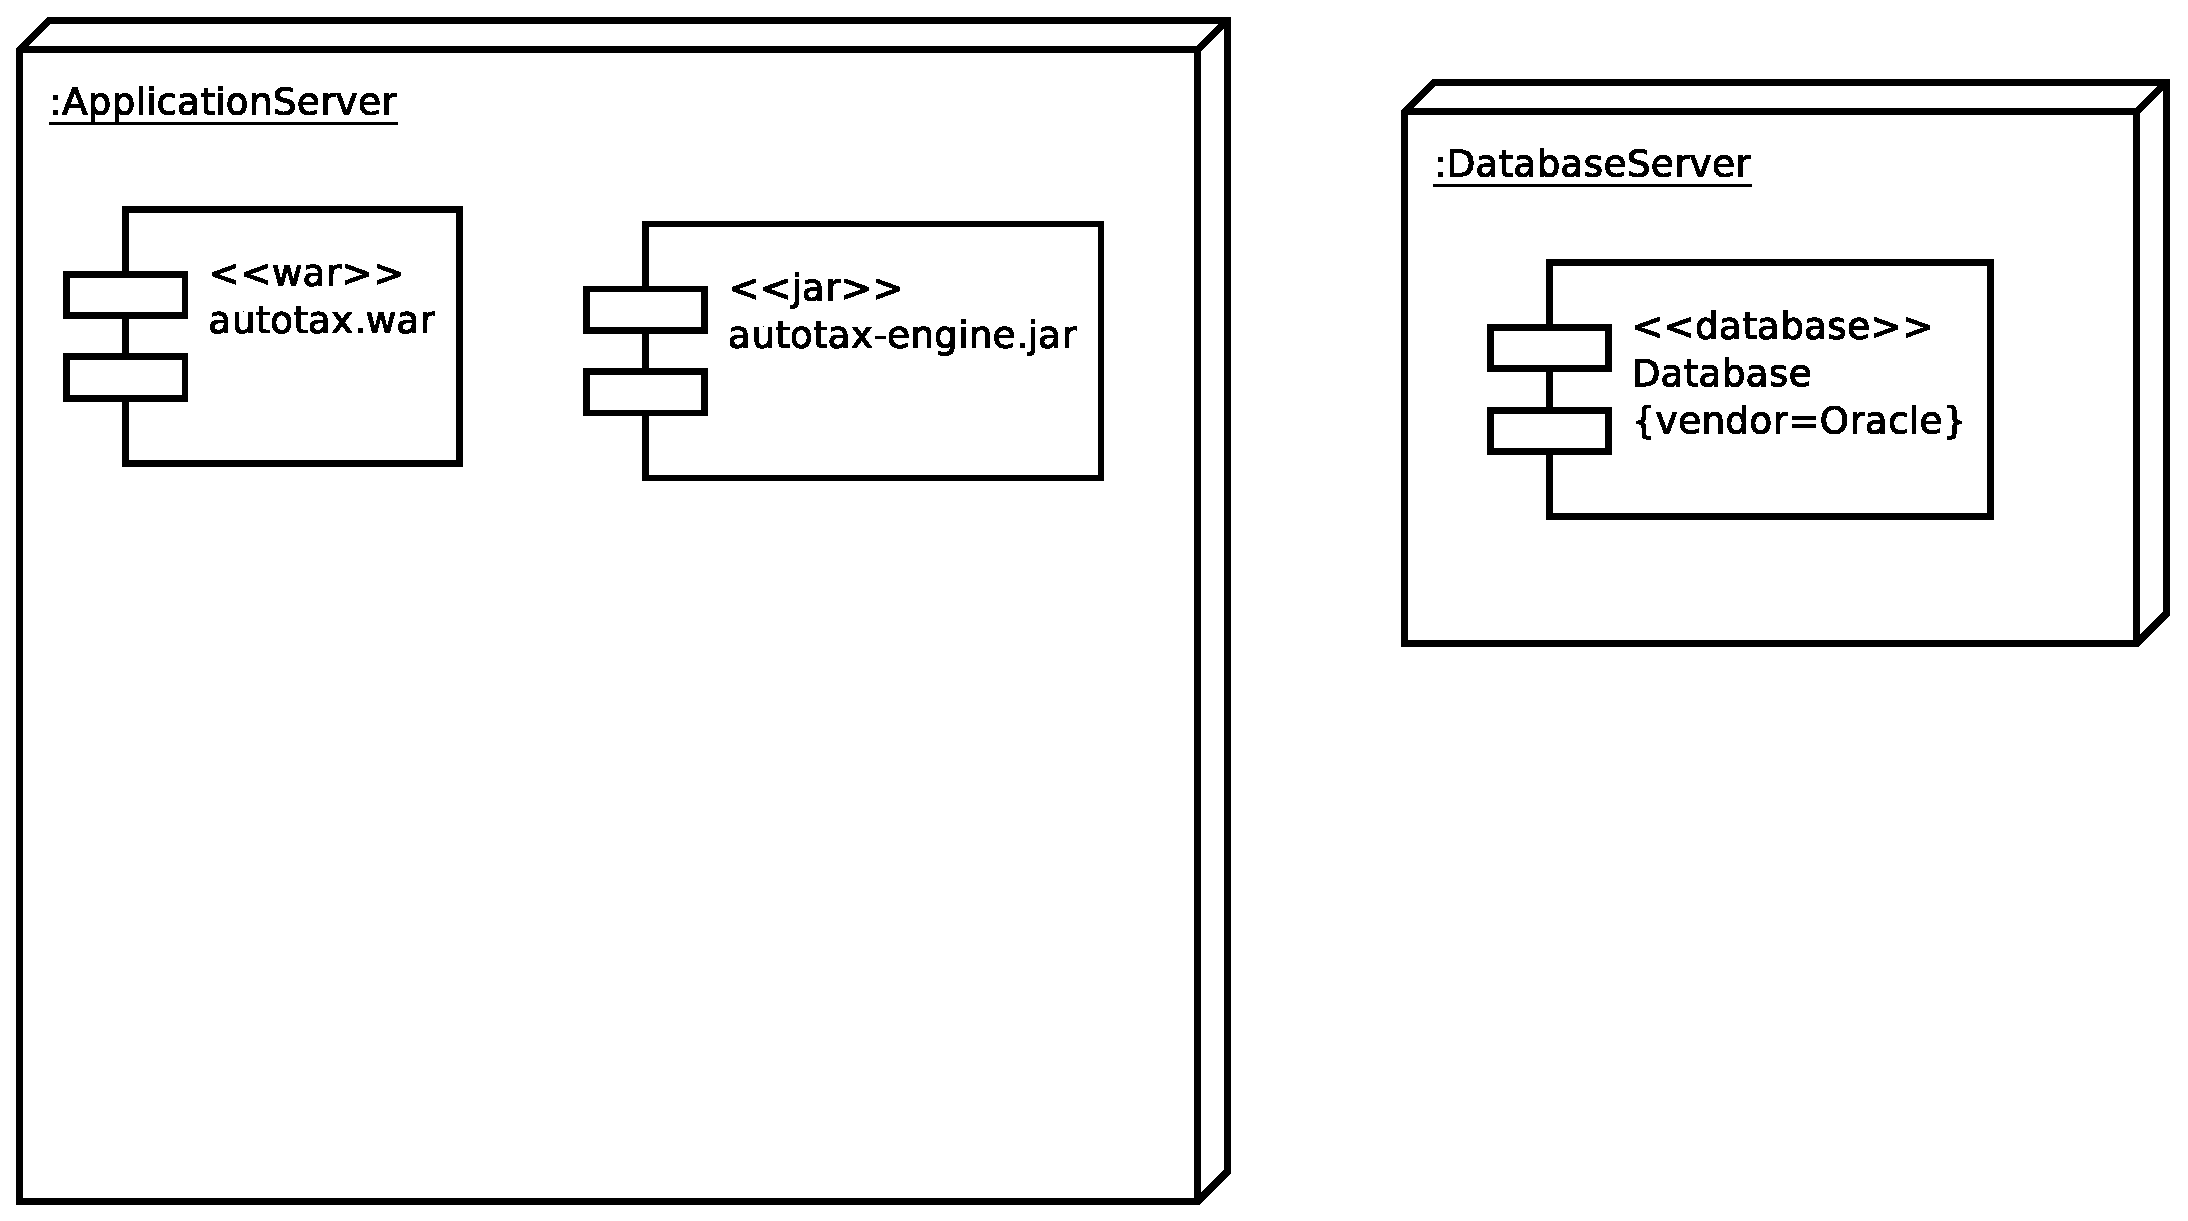
\includegraphics[scale=0.34]{uml/deployment}
  \caption{Диаграмма развертывания системы}
  \label{pic:deployment}
\end{figure}

Диаграмма компонентов системы представлена на рисунке~\ref{pic:componentsdiagram}. Было реализовано шесть компонентов:
\begin{gostitemize}
\gostitem{подсистема управления декларацией --- подсистема представляет собой набор классов для управление декларацией, что включает в себя загрузку структуры декларации, подсчет декларации, пересчет отдельных ячеек декларации;}
\gostitem{подсистема вычисления выражений --- набор классов, которые осуществляют подсчет выражения на формальном языке, данная подсистема используется подсистемой управления декларацией для подсчета формульного типа ячеек;}
\gostitem{подсистема управления --- подсистема <<связывает>> остальные подсистемы, занимается обработкой запросов;}
\gostitem{подсистема хранения --- подсистема, предоставляющая возможность сохранения, загрузки и обновления объектов, которые находятся в базе данных, для реализации данной подсистемы использовалась библиотека Hibernate;}
\gostitem{подсистема отображения --- подсистема, предоставляющая пользователю интерфейс для взаимодействия с системой;}
\gostitem{модель --- содержит классы, представляющие собой сущности предметной области, такие как <<Компания>>, <<Налоговые Формы>>, <<Бухгалтерская Книга>>, <<Счет>>, <<Ячейка>> и т.д.}
\end{gostitemize}

\begin{figure}
  \centering
  \includegraphics[scale=0.4]{uml/componentsdiagram}
  \caption{Диаграмма компонентов системы}
  \label{pic:componentsdiagram}
\end{figure}

\subsection{Реализация модельных классов}
На рисунке~\ref{pic:model_classes} приведены модельные классы и отношения между ними. Рассмотрим данные классы в контексте выделенных на этапе проектирования объектов.

\gostitemi{класс Cell - представляет ячейку, имеет атрибуты: <<name>>- имя ячейки, <<state>> -состояние ячейки, <<valueType>> - тип зачения;}
\gostitemi{класс CellState - представляет состояние ячейки, имеет атрибуты: <<types>> - список возможны типов ячейки (экземпляры класса CellType), \mbox{<<cellValue>>} - значение, <<activeType>> - текущий тип ячейки. Атрибут <<name>> (имя) был введен, так как данный объект будет отражен на соответсвующую таблицу в базе данных, при отображений из записи в таблице базы данных на данный объект необходимо его сопоставить с соответствующим экземпляром класса <<Cell>>. Атрибут <<id>> является уникальным идентификатором;}
\gostitemi{класс CellValue - представляет значение ячейки, имеет атрибуты: <<id>> - уникальный идентификатор, <<doubleValue>> - вещественное значение,\\ <<longValue>> - целочисленное значение, <<stringValue>> - строковое значение, <<valueType>> - тип хранимого значения (целочисленный, строковый либо вещественный);}
\gostitemi{класс Report - представляет декларацию, содержит атрибуты: <<name>> - имя декларации, <<Cell>> - множество ячеек, <<crossReports>> - список деклараций, от которых зависит значения ячеек данной декларации (в формульной ячейке может использоваться переменная, которая содержит значение ячейки из другой декларации), <<reportState>> - состояние декларации;}
\gostitemi{класс ReportState --- представляет состояние декларации. Содержит атрибуты: <<id>> - уникальный идентификатор;}
\gostitemi{класс CellType --- абстрактный класс, представляет тип ячейки;}
\gostitemi{класс CellTypeAccounts --- расширяет класс CellType, представляет собой тип ячейки <<Счета>>;}
\gostitemi{класс CellTypeEditable --- расширяет класс CellType, представляет собой тип ячейки <<Пользовательская>>;}
\gostitemi{класс CellTypeFormula --- расширяет класс CellType, представляет собой тип ячейки <<Формула>>;}
\gostitemi{класс Account --- представляет интервал, атрибуты: <<accFrom>> - начало интервала, <<accTo>> - конец интервала, <<sign>> --- знак (<<+>> либо <<->>), <<type>> - тип (дебет либо кредит);}
\gostitemi{класс Company --- представляет компанию, параметры: <<id>> - уникальный идентификатор, <<name>> - название компании, <<code>> - код компании;}
\gostitemi{класс TaxKit --- представляет налоговые формы, <<id>> - уникальный идентификатор, <<name>> - имя, <<selected>> - показыват выбраны ли данные налоговые формы в качестве текущих, <<ledger>> - бухгалтерская книга, счета которой будут использоваться для подсчета соответствующих ячеек деклараций, <<company>> - компания, которой принадлежат данные налоговые формы;}
\gostitemi{класс Ledger --- представляет бухгалтерскую книгу, <<id>> - уникальный идентификатор, <<name>> - имя, <<company>> - компания, которой принадлежит бухгалтерская книга, <<accounts>> - список счетов, принадлежащих бухгалтерской книге;}
\gostitemi{класс LedgerAccount --- представляет запись в бухгалтерской книге\\ (<<Счет>>), <<debit>> - значение дебета для счета, <<credit>> - значение кредита для счета, <<number>> - номер счета.}

\begin{sidewaysfigure}
  \centering
  \includegraphics[scale=0.4]{uml/impl_model}
  \caption{Диаграмма модельных классов}
  \label{pic:model_classes}
\end{sidewaysfigure}

\subsection{Реализация подсистемы управления декларацией}

На рисунке~\ref{pic:loadclasses} изображена диаграмма классов для загрузки декларации. Абстрактный класс ReportLoader содержит абстрактный метод <<load>> для загрузки структуры декларации, данный метод имеет параметр <<name>>, который показывает имя деклапации. XMLReportLoader реализует метод <<load>> класса ReportLoader, для разгрузки декларации из XML документа. Атрибут <<reportRegistry>> ссылается на ReportRegistry, абстрактный класс, метод <<get>> которого возвращает путь типа java.net.URL который указывает на XML документ, который описывает структуру диаграммы. Класс XMLReportRegistry реализует метод <<load>> абстрактного класса ReportRegistry для загрузки декларации с файловой системы, атрибут <<path>> показывает путь к директории, в которой хранятся XML документы.

\begin{figure}
  \centering
  \includegraphics[scale=0.35]{uml/impl_classes1}
  \caption{Диаграмма классов для загрузки декларации}
  \label{pic:loadclasses}
\end{figure}

На рисунке~\ref{pic:reportmanager} изображена диаграмма классов, участвующих в управлении декларацией. Класс ReportManager представляет методы для работы с декларацией. Для создания экземпляра класса ReportManager, в качестве параметра конструктора необходимо передать экземпляр класса Report (уже загруженной структуры декларации). Класс ReportInterpreter используется для подсчета ячеек декларации. Класс CellInterpreter содержит абстрактный метод <<calculate>>, который подсчитывает значение ячейки для заданного типа, метод в качестве параметров принимает экземпляры класса CellType и Context, Context используется для получения значений других ячеек данного отчета.

\begin{sidewaysfigure}
  \centering
  \includegraphics[scale=0.4]{uml/impl_classes2}
  \caption{Диаграмма классов для управления декларацией}
  \label{pic:reportmanager}
\end{sidewaysfigure}

\subsection{Реализация подсистемы вычисления выражений}

Приведем классы, которые отвечают за вычисление выражений (рисунок~\ref{pic:evalclasses}). Класс ExpressionLexer выполняет лексический анализ выражения (expression), метод lex возвращает следующую лексему, были выделены следующие лексемы:

\begin{itemize}
  \itemцелое число(INTEGER);
  \itemвещественное число (DOUBLE);
  \itemстрока (STRING);
  \itemразделитель (DELIMETER);
  \itemпеременная (VARIABLE);
  \itemидентификатор (IDENTIFIER);
  \itemконец выражения (EOF);
\end{itemize}

Класс ExpressionParser выполняет синтаксический анализ на основе лексем, которые были созданы в результате лексического анализа. Для реализациия синтаксического анализатора использовался метод нисходящего рекурсивного парсека. Суть метода заключается во взаимном вызове анализирующих процедур, соответствующих правилам грамматики. Приведем методы, которые отвечают за анализ правил грамматики:

\begin{gostitemize}
  \gostitem{метод parse анализирует выражение;}
  \gostitem{метод parseSubExpr анализирует вложенное выражение, в качестве первого параметра принимает левую часть выражения, в качестве второго параметра - минимальный допустимый приоритет, вложенное выражение может включать в операторы, как бинарные, так и унарные, для разбора простых выражений использует метод parseSimpleExpr;}
  \gostitem{метод parseSimpleExpr анализирует простое выражение: целое, вещественное, переменная, константа, идетификатор, вызов функции;}
  \gostitem{метод parseFuncCall анализирует выражение для вызова функции;}
  \gostitem{метод parseFuncParam анализирует выражение для параметра функции.}
\end{gostitemize}
Метод parse возвращает абстрактное синтаксическое дерево, которое представлено реализациями класса AST:

\begin{itemize}
  \itemбинарная операция (BinOp);
  \itemвызов функции (FuncCallAST);
  \itemпараметр функции (FuncParamAST);
  \itemлитерал (LiteralAST);
  \itemчисло (NumberAST);
  \itemунарная операция (UnaryOpAST);
  \itemпеременная (VariableAST).
\end{itemize}

Класс EvaluationVisitor, является реализацией шаблона проектирования <<Посетитель>> \cite{patterni}. Реализация каждого узла содержит метод visit, в качестве параметра ему передается экземпляр посетителя, в данном методе должен производится вызов соответствующего метода посетителя, например в реализации BinOp метод visit вызывает метод visitBinOp, передает ему в качестве параметра текущий экземпляр (this в java). Таким образом, для обхода всего АСД необходимо вызвать метод visit у корневого элемента (элемента, который возвращается в качестве результата синтаксического анализа) передав ему в качестве параметра экземпляр класса EvaluationVisitor.

\begin{sidewaysfigure}
  \centering
  \includegraphics[scale=0.4]{uml/impl_classes3}
  \caption{Диаграмма классов для вычисления значения выражения}
  \label{pic:evalclasses}
\end{sidewaysfigure}

Класс ExpressionEval для вычисления значения выражения предоставляет метод eval, в качестве параметра ему передается строковое выражение(expression). Данный класс использует ExpressionParser для создания АСД, EvaluationVisitor, для получения значения выражения.

\subsection{Реализация подсистемы управления}

Классы подсистемы управления занимаются обработкой запросов и обеспечивают взаимодействие остальных подсистем.


Для обработки запросов используется модуль Spring MVC фреймворка Spring. Spring MVC использует контроллер, который представляет собой сервлет (<<DispatcherServlet>>) который обрабатывает запрос делегирует обработку запроса соответствующему контроллеру. Декларация контроллеров, которые должны обрабатывать соответствующие запросы осуществляется в конфигурационном файле.


Контроллером является класс, который содержит методы для обработки запросов. Описанные методы должны возвращать экземпляр класса <<ModelAndView>>, который содрежит название представления (<<View>>) и карту, содержащую параметры, которые будут переданы подсистеме отображения, ключем является название параметра (строка), а значением может быть экземпляр любого класса. Выполнения метода контроллера обрабатывающего запрос, управление передается подсистеме отображения, подсистема отображения <<Spring MVC>> по названию. Процесс обработки запроса представлен на рисунке~\ref{pic:springmvcref}.


\begin{figure}
  \centering
  \includegraphics[scale=0.5]{uml/spring_mvc_req}
  \caption{Процесс обрабоки запроса Spring MVC}
  \label{pic:springmvcref}
\end{figure}


В рамках подсистемы управления реализованы следующие контроллеры:
\begin{gostitemize}
  \gostitem{CompanyController - содержит методы для обработки запросов на отображение списка доступных компаний, для отображения компании, метод для удаления компании. Метод для отображения списка компаний в качестве модельных данных возвращает список объектов <<Company>>, которые загружаются из базы данных с использованием подсистемы хранения. Метод для отображения компании, в зависимости от параметра <<id>> запроса, посредством подсистемы хранения получает экземпляр класса <<Company>>, который передается соответствующей JSP странице для отображения;}
  \gostitem{класс LedgerController - содержит методы для обработки запросов на отображения списка доступных бухгалтерских книг, для отображения свойств конкретной бухгалтерской книги, для отображения формы редактирования бухгалтерской книги, для создания бухгалтерской книги;}
  \gostitem{класс ReportController - содержит метод для обработки запросов на отображение декларации. При обработке запроса на отображение декларации, посредством подсистемы управления декларацией, создает нужную декларацию и передает структуру декларации подсистеме отображения;}
  \gostitem{класс ReportStateController - содержит методы для обработки запросов на получения состояния ячеек декларации, на пересчет ячейки и зависимых ячеек, на изменение типа ячейки, на сохранение состояния декларации. Для получения состояния ячеек используется подсистема хранения, посредством которой получается сохраненный объект <<ReportState>>. Для получения объекта <<ReportState>> необходимы идентификатор выбранных налоговых форм и название текущей декларации, данные параметры должны находиться в запросе;}
  \gostitem{класс TaxKitController - содержит методы для отображения списка налоговых форм (<<TaxKit>>), для удаления наловых форм. Данные действия производятся посредством подсистемы хранения;}
  \gostitem{класс TaxKitCreateController - содержит методы для создания налоговых форм. Метод для обработки запроса на отображения формы создания налоговых форм возвращает название соответствующей страницы. Метод для обработки запроса на добавления налоговых форм, на основании параметров, переданных формой создания создает новые налоговые формы;}
  \gostitem{класс TaxKitEditController - содердит методы для редактирования налоговых форм. Метод для обработки запросы на отображение формы редактирования возвращает название соответствующей страницы, в качестве модельных данных возвращает экземпляр налоговых форм, который был получен посредством подсистемы хранения;}
\end{gostitemize}

\subsection{Реализация подсистемы хранения}

Подсистема хранения используется для добавления, получения и удаления сущностей системы из базы данных. На таблицы в базе данных отображаются следующие классы: ReportState, CellState, CellTypeFormula, CellTypeAccounts, CellTypeEditable, Account, CellValue, TaxKit, Company, Ledger, LedgerAccount. Данная подсистема была реализована с использованием библиотеки Hibernate. Каждый объект был отображен на соответствующую таблицу в базе данных, так же отображены связи между объектами. Примитивные типы данных Java отображаются на типы данных SQL.

На рисунке~\ref{pic:ormsample} рассмотрим отображение объектов <<ReportState>> и\\ <<CellState>> на таблицы в базе данных. Класс <<ReportState>> отображен на таблицу <<REPORTSTATE>>, атрибут <<id>> класса <<ReportState>> отображен в соответствующий атрибут таблицы и является первичным ключом. Класс <<CellState>> отображен на таблицу <<CELLSTATE>>, у данной таблицы есть атрибут <<REPORTSTATE\_ID>> который является внешним ключом, ссылающимся на атрибут <<ID>> таблицы <<REPORTSTATE>> данная ссылка отображает отношение <<ReportState>> к <<CellState>> как 1:n.

\begin{figure}
  \centering
  \includegraphics[scale=0.4]{uml/ormsample}
  \caption{Отображение классов <<ReportState>>, <<CellState>> и связи между ними на таблицы в базе данных}
  \label{pic:ormsample}
\end{figure}


\subsection{Реализация подсистемы отображения}
Подсистема отображения предоставляет пользователю интерфейс для общения с системой. Разработаная система является веб-приложением, которое предоставляет пользователю интерфейс, представленный набором интерактивных веб страниц. Для реализации веб-страниц использовалась технология JSP. JSP страница является текстовым документом, которая содержит текст двух типов: статические исходные данные, которые могут быть оформлены в одном из текстовых форматов HTML, SVG, WML, или XML, и JSP элементы, которые конструируют динамическое содержимое. Кроме этого могут использоваться библиотеки JSP тегов для внедрения Java-кода. JSP --- одна из высокопроизводительных технологий, так как весь код страницы транслируется в java-код сервлета с помощью компилятора JSP страниц Jasper, и затем компилируется в байт-код виртуальной машины java.

Для реализации страниц использовался язык сценариев JavaScript \cite{jsprogr}, с помощтю которого можно изменять структуру страниц динамически. Для асинхронной работы с сервером использовалась технология AJAX \cite{ajaxmast}, которая позволяет диамически обращаться к серверу, без перезарузки страницы. В качестве формата передачи данных используется язык JSON. Сценарий на языке JavaScript обращается к серверу для получения каких либо данных, контроллер обрабатывает запрос и в качестве ответа возвращает не название представления, а ответ на языке JSON.


Подсистему отображения реализованой системы можно разделить на два класса: отображение форм, списков сущностей (<<Компания>>, <<Набор Деклараций>>, <<Бухгалтерская Книга>>) и отображение отчетов.


Для реализации форм отображения и списков сущностей были написаны соответсвующие jsp страницы. Контроллер для соответствующей сущности передает список объектов в качестве модельных данных, а jsp страница выводит этот список. На рисунке~\ref{pic:taxkits_list} представлена страница со списком <<Налоговых Форм>>. После обработки запроса на отображения списка налоговых форм, TaxKitsController возвращает список доступных форм в качестве модельных данных. При обработке запроса на редактирование/создание сущности, контроллер возвращает сущность в качестве модельных данных (~на рисунке~\ref{pic:ledger_creation} представлена форма создания <<Бухгалтерской Книги>>~), при создании контроллер возвращает экземпляр сущности, с пустыми полями, а при редактировании, посредством подсистемы хранения, из базы данных получается соответсвующий объект и передается jsp странице. После редактирования контроллер обрабатывает запрос на сохранение сущности, значения аттрибутов передаются в HTTP запросе. При редактировании и создании <<Бухгалтерской Книги>> использовалась технология AJAX. Контроллер LedgerController содержит методы insertAccount и removeAccount, которые обрабатывают асинхронные запросы со страницы редактирования(либо создания) <<Бухгалтерской Книги>>, для добавления и удаления счета соответсвенно.


\begin{figure}
  \centering
  \includegraphics[scale=0.43]{pics/scr_taxkit_list}
  \caption{Список доступных <<Налоговых Форм>>}
  \label{pic:taxkits_list}
\end{figure}

\begin{figure}
  \centering
  \includegraphics[scale=0.43]{pics/scr_ledger_creation}
  \caption{Форма создания <<Бухгалтерской Книги>>}
  \label{pic:ledger_creation}
\end{figure}

Каждая налоговая декларация имеет визуальное представление в XSLT документе. XSLT --- часть спецификации XSL, задающая язык преобразований XML-документов. При применении таблицы стилей XSLT, состоящей из набора шаблонов, к XML-документу образуется конечное дерево, которое может быть другой XML-структурой, HTML-документом или обычным текстом. В качестве XML документа используется представление структуры декларации, а конечным деревом является HTML документ, который представляет собой отображение декларации. Для того, что бы получить XSLT документ, который является представлением конкретной декларации используется реализация интерфейса ReportViewResolver, данный интерфейс содержит метод resolve, в качестве параметров которому передается экземпляр класса Report, метод возвращает путь к XSLT документу.

При редактировании ячейки пользователем, на сервер отправляются асинхронные запросы на языке JSON, которые содержат информацию о изменяемой ячейке:
\begin{lstlisting}[language=Python,basicstyle=\small]
{ "cellValueDTO":{
      "strValue":"0"
   },
   "name":"CELL2"
}
\end{lstlisting}

В качестве ответа, сервер отправляет список пересчитанных ячеек со значениями:
\begin{lstlisting}[language=Python,basicstyle=\small]
[   {"name":"CELL3",
     "type":"formula",
     "stateDTO":
          {"name":null,
           "valueType":"LONG",
           "cellValueDTO":{
                "actualValue":222222,
                "strValue":"222222"
             }
          } },
    {"name":"CELL2",
     "type":"editable",
     "stateDTO":
          {"name":null,
           "valueType":"LONG",
           "cellValueDTO":{
                "actualValue":0,
                "strValue":"0"
            }
     }}
]
\end{lstlisting}

Методы, которые обрабатывают асинхронные запросы для пересчета ячеек находяться в классе ReportStateController: метод recalculateCell обрабатывает запрос на пересчет ячейки, в рамках измененного значения; метод changeState обрабатывает запрос на изменения состояние ячейки.


\begin{figure}
  \centering
  \includegraphics[width=16cm]{pics/scr_reportrules_nice}
  \caption{Страница с декларацией, редактирование ячейки типа <<Счета>>}
  \label{pic:report_scr}
\end{figure}

\subsection{Физическая модель базы данных}
Представим физическую модель базы данных(рисунок~\ref{pic:database}, которая была построена на основании логической модели. Схема базы данных содержит двенадцать таблиц, каждая таблица соотсветсвует классу модели.


Каждая таблица имеет свой первичный ключ --- минимальное множество атрибутов, являющееся подмножеством заголовка данного отношения, составное значение которых уникально определяет кортеж отношения, в данном случае аттрибут один у каждой таблицы один. Таблицы связаны друг с другом с помощью внешних ключей. Внешним ключом называется поле таблицы, предназначенное для хранения значения первичного ключа другой таблицы с целью организации связи между этими таблицами. Например для реализации отношения 1:n таблиц REPORTSTATE и CELLSTATE, в таблице CELLSTATE присутствует внешний ключ REPORT\_STATE\_ID, который ссылается на первичный ключ(ID) таблицы REPORTSTATE.


Таблицы CELLTYPEEDITABLE, CELLTYPEFORMULA, \\CELLTYPEACCOUNTS являются отображениями классов CellTypeEditable, CellTypeFormula, CellTypeAccount, которые наследуются от класса CellType (который отображен на таблицу CELLTYPE). Опишем отображение наследования. У кажой из таблиц, на которые отображены классы-наследникаи есть первичный ключ ID, который является внешним ключем и ссылается на аттрибут ID таблицы CELLTYPE, который так же является первичным ключем. Аттрибуты ACTIVETYPE (показывает активен ли данный тип для состояния ячеки), TYPE (название типа) и CELLSTATE\_ID(внешний ключ, ссылающийся на первичный ключ ID таблицы CELLSTATE), которые присутствуют у всех наследников находятся в таблице CELLTYPE. Таким образом, по записи в таблице CELLTYPE можно однозначно определить, какой из потомков объекта CellType отражен в данных таблицах.
\begin{figure}[ht]
  \centering
  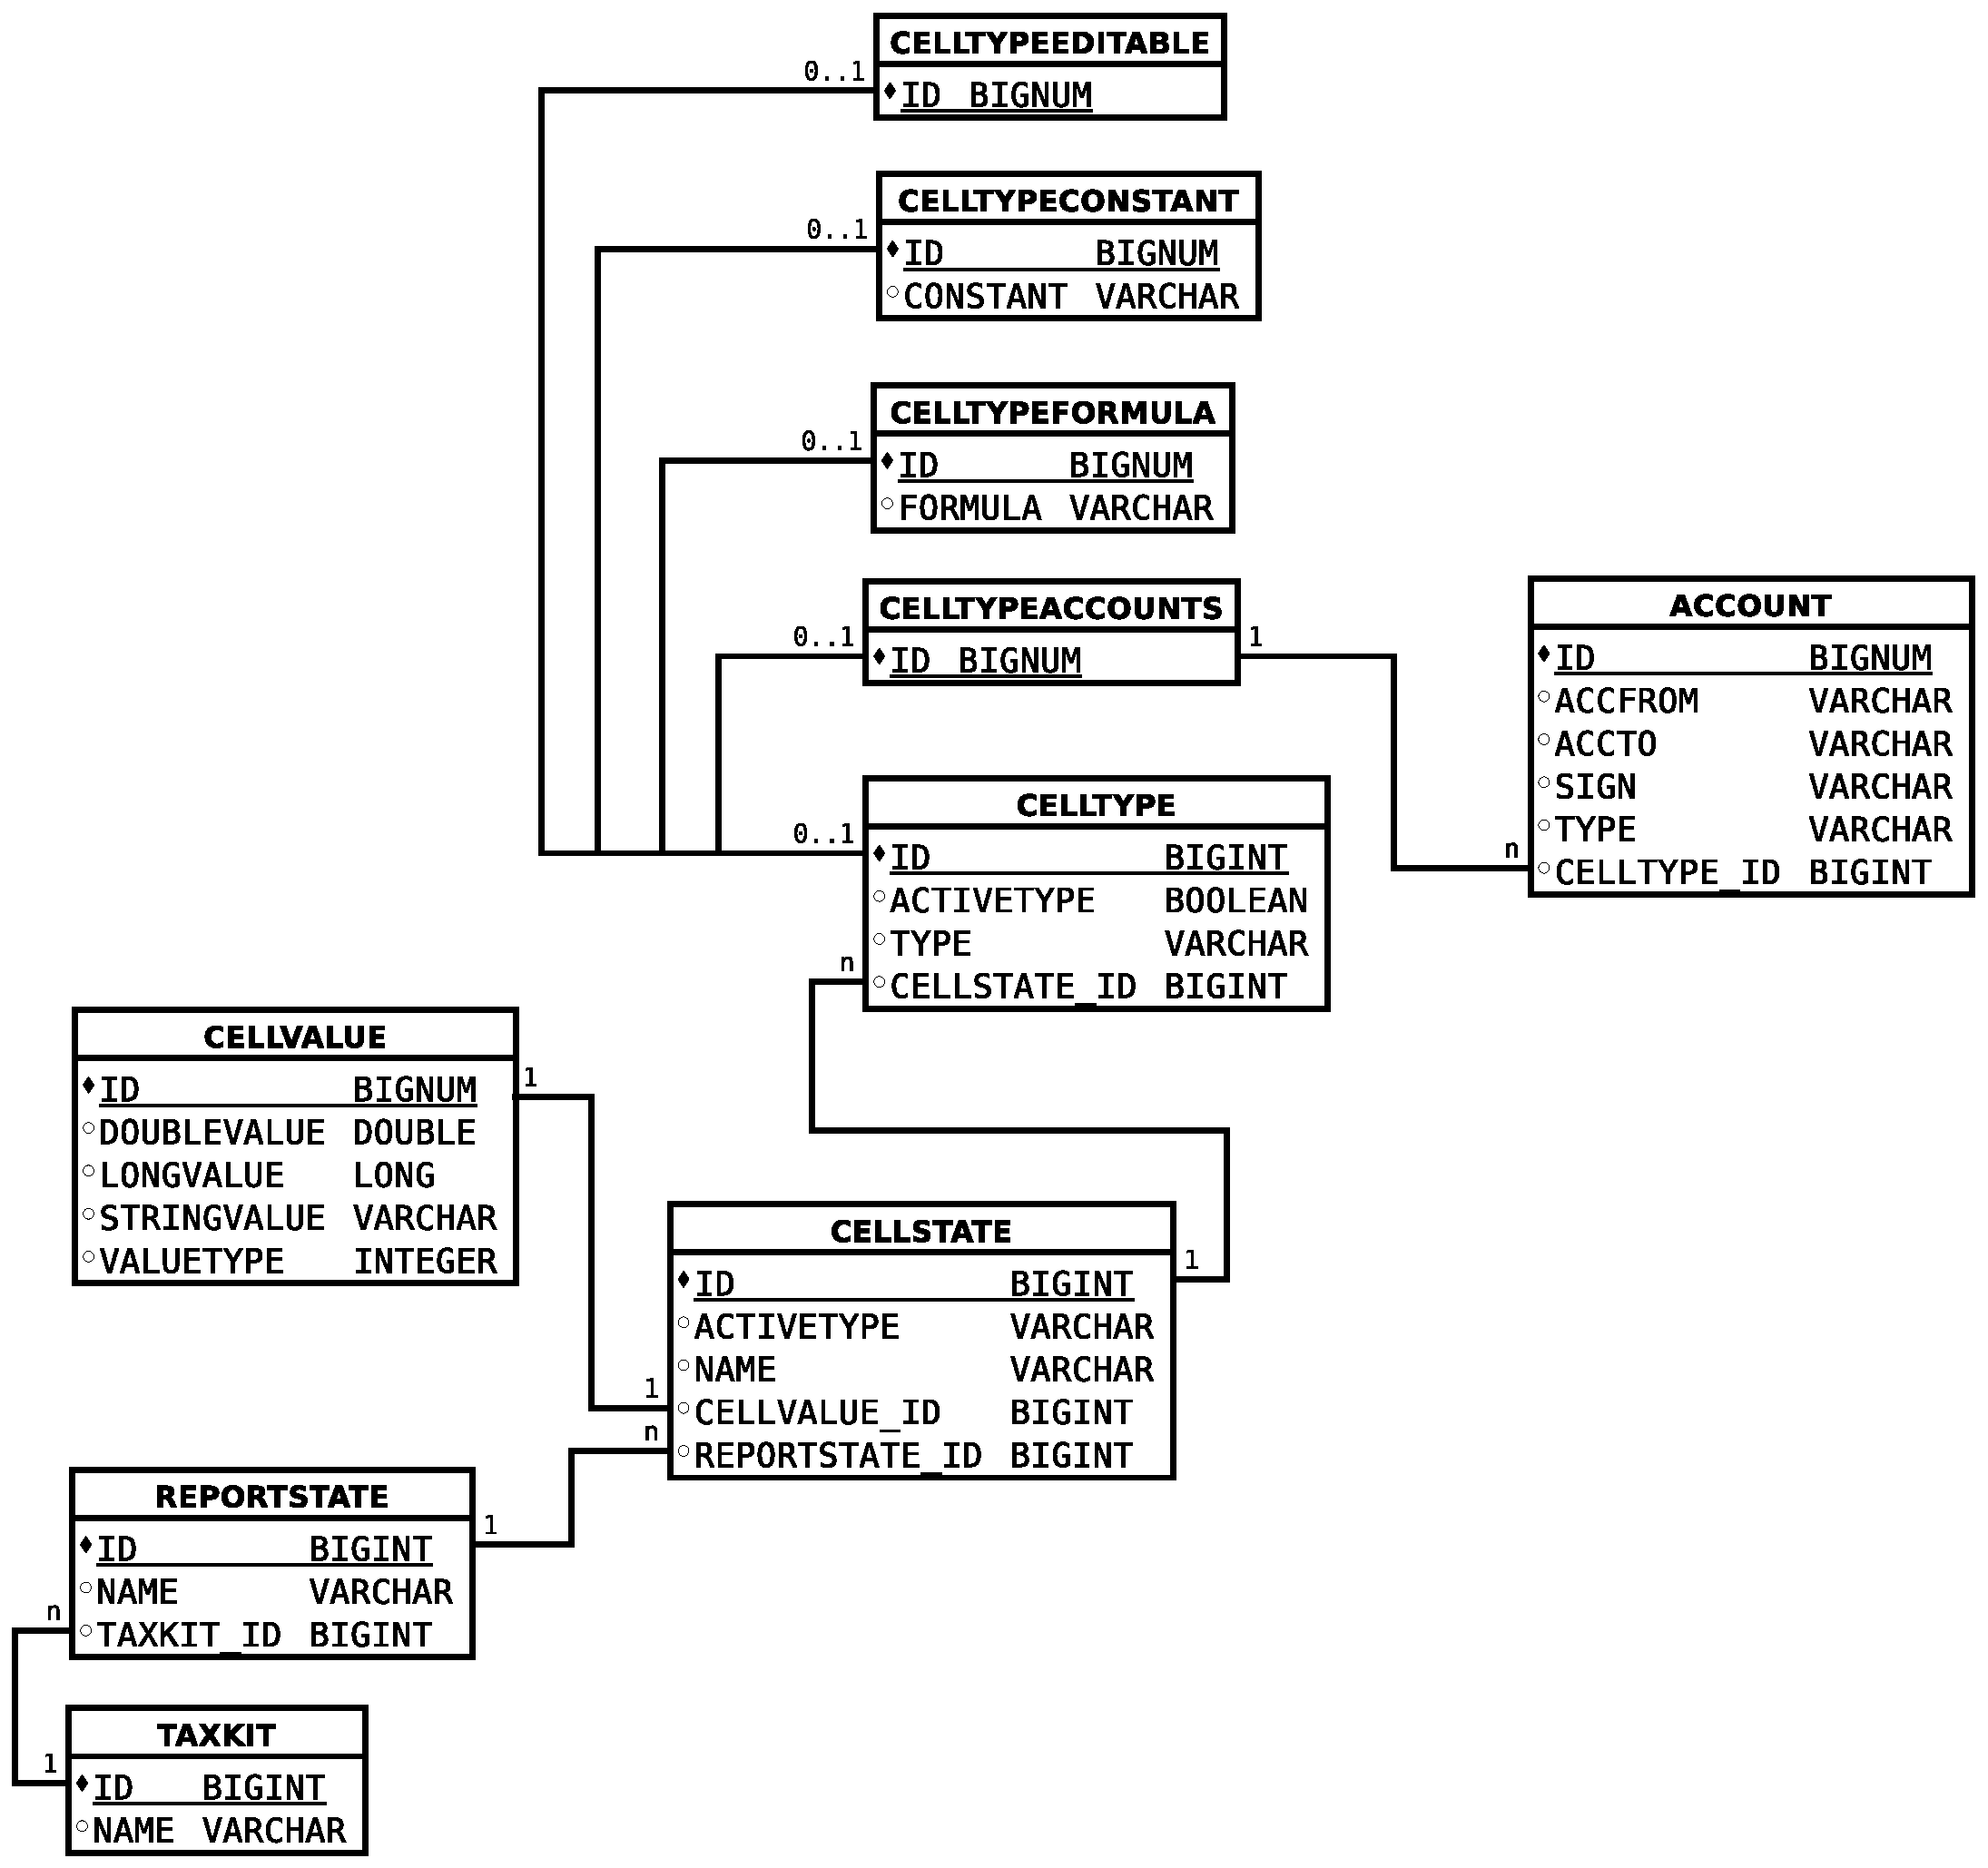
\includegraphics[scale=0.4]{uml/database}
  \caption{Физическая модель базы данных}
  \label{pic:database}
\end{figure}

\section{Тестирование}
В целях тестирования кода и контроля качества во время разработки были написаны модульные тесты. Тесты представляют собой набор утверждений, которые не должны быть опровергнуты в результате ожидаемой (корректной) работы тестируемого модуля. В данном контексте модулем является тестируемый класс. Наборы утверждений объединяются в методах. В рамках соглашения был использован следующий формат имени метода: <<testMethod>>, где Method - название тестируемого метода.


Для написания тестов были использованы XML документы, которые содержат структуры следущих отчетов: <<states>>, <<cross-report-1>>, <<test-calc>>, данные документы приведены в Приложении А.

Опишем классы, которые представляют собой модульные тесты. Класс XMLReportLoaderTest тестирует загрузку декларации из формата XML. Для тестирования был создан XML файл, который содержит представление структуры отчета. Производится загрузка декларации из XML документа (<<states>>), при положительном исходе, должна получиться декларация, которая содержит пять ячеек. Имена ячеек, описанных в XML документе должны совпадать со значением аттрибутов name каждого экземпляра класса Cell, экземпляры класса CellState должны содержать список возможных типов (аттрибут types) соотсветсвующий определенному списку в XML документе.


Для тестирования подсчета декларации используется класс ReportInterpreterTest. Для тестирования загружается декларация из XML документа. В качестве значения ячейки <<CELL1>> устанавливается 1,  <<CELL2>> устанавливается 3. Значение ячейки <<CELL3>> должно быть равно 4, так как значение данной ячейки вычисляется по формуле \$\{CELL1\}+\$\{CELL2\}. После изменения значения ячейки <<CELL1>> на 4 и пересчета зависымых ячеек, должна пересчитаться ячейка <<CELL3>> и её значение должно быть равно 7.


Для тестирования подсчета формулы, которая зависит от ячеек, которые находятся в другой декларации был написан класс ReportCrossInterpreterTest. Загружается декларация <<cross-calc-1>>, которая содержит ячейки <<CELL1>> - пользовательская ячейка, <<CELL4>> - ячейка с формулой: \mbox{\$\{states.CELL1\}+\$\{CELL2\}}. Для декларации <<states>> значение ячейки <<CELL1>> устанавливается 2, для декларации <<cross-calc-1>> значение ячейки <<CELL1>> устанавливается 3. При подсчете ячейки <<CELL4>> декларации <<cross-report-1>> должно получится значение 5.


Для тестирования подсчета ячеек типа <<Cчета>> был написан класс AccountsInterpreterTest. Были созданы следующие счета для бухгалтерской книги:
\begin{itemize}
  \item Номер: <<123>> дебет: 2, кредит 3
  \item Номер: <<125>> дебет: 0, кредит 3
  \item Номер: <<333>> дебет: 0, кредит 3
\end{itemize}
Для ячейки были созданы следующие интервалы:
\begin{itemize}
  \item От 111 до 125 знак + тип: дебет
  \item От 111 до 333 знак - тип: кредит
\end{itemize}
После подсчета данной ячейки должно получится значение -7, так как в первый интервал попадают счета с номером <<123>> и <<125>>, тип дебет и суммарное значение равно 2, во второй интервал попадают все интервалы, тип кредит, суммарное значение равно -9 (с учетом знака). Получается сумма 2+(-9) = -7.

Для тестирования методов редактирования отчета, которые реализованы в классе ReportManager был реализован класс ReportManagerTest. Создается декларация <<test-calc>>, содержащая три ячейки: <<CELL1>> - пользовательская, <<CELL2>> - пользовательская, <<CELL3>> - формульная, формула: \$\{CELL1\}+\$\{CELL2\}. Значения ячеек <<CELL1>> и <<CELL2>> устанавливаются 1 и 2 соответственно. Проводится тестирование изменение типа ячейки с формульной на пользовательскую. Подсчитывается значение формульной ячейки, которое должно быть равно 3. Далее тип ячейки <<CELL3>> изменяется на пользовательскую, значение ячейки <<CELL1>> устанавливается 4, пересчитывается значение ячейки <<CELL3>>, оно должно быть равно прежнему значению 3, так как тип уже не формульый, а пользовательский, и подсчитанное значение равно 3. Далее тип ячейки <<CELL3>> меняется с пользовательской на формульную и пересчитывается значение, которое равно 6, так как значение вычисляется уже по формуле.


Для тестирования контроллера ReportStateController, который обрабатывает запросы на редактирование декларации был написан класс ReportStateControllerTest. Для тестирования были созданы сущности: компания, бухгалтерская книга, налоговые формы. Далее обрабатывается запрос на открытие декларации <<test-calc>> для созданных налоговых форм. Контроллер должен передать клиенту ответ на языке JSON, который соответсвует пустому состоянию декларации (все ячейки имеют нулевые значения). Оправляется запрос на изменение значение ячейки <<CELL1>>, которой установлено значение 101, в качестве ответа, контроллер должен вернуть список представленный на языке JSON, который содержит новое значение ячейки <<CELL3>>, новое значение должно равняться 101. Далее отправляется запрос на сохранение декларации. Затем декларация открывается заново, после обработки запроса на открытие декларации, контроллер должен вернуть сохраненное состояние декларации, значение ячейки <<CELL1>> должно быть установлено как 101 и значение ячейки <<CELL3>> должно быть установлено как 101.


Результаты  выполнения тестов, которые содержаться в описанных выше классах, положительны.

\chapter{Охрана труда, экологическая безопасность, энергосбережение}

\section{Обеспечение комфортных условий труда разработчиков систем электронного документооборота}
Все стадии разработки данного дипломного проекта проводились на предприятии ЗАО <<Итранзишен>>.


К умственному труду (интеллектуальному труду) относится деятельность, связанная с приемом и переработкой информации, требующая напряженного функционирования процессов внимания, памяти, мышления, эмоциональной сферы. Научно-технический прогресс с каждым годом увеличивает число лиц, выполняющих преимущественно умственную работу. У многих профессий с традиционным преобладанием физического труда в настоящее время имеется стойкая тенденция к увеличению доли умственного компонента. Для большинства современных профессий характерны ускоренный темп, резкое увеличение объема информации, дефицит времени для принятия решений, возрастание социальной значимости этих решений и личной ответственности. Перечисленные факторы часто приводят к нервным перегрузкам, а как следствие — к возникновению сердечно-сосудистых и нервных заболеваний.


При умственном труде мозг --- это не только регулирующий, но и работающий орган, поэтому влияние интеллектуальных нагрузок сказывается прежде всего на функциональном состоянии центральной нервной системы. Основное условие стабильного трудового процесса при умственной работе --- это выработка и поддержание устойчивой доминанты, обесценивающей высокий уровень работоспособности.


Напряженность умственной деятельности --- это характеристика труда, отражающая физиологическую стоимость нагрузки при психической работе. Основной причиной повышенной напряженности и возникающих в результате этого нарушений адекватной регуляции функций являются перегрузки чувствительных, центральных и исполнительных звеньев функциональных систем, осуществляющих трудовую деятельность. Это происходит, в частности, при различении человеком близких по параметрам сигналов, попытках выделить полезный сигнал из шума, выполнении предельно точных и четких движений, необходимости принять решение с альтернативным выбором в условиях дефицита времени.


Работающий мозг потребляет значительно больше кислорода, чем другие ткани тела. Обмен веществ и энергии мозга в состоянии покоя составляет в среднем 35 калорий в минуту или всего 3\% от общего обмена в организме. Возрастание интенсивности умственной работы сопровождается усилением расхода энергии (таблица~\ref{table:energy}).

\begin{table}[ht]
  \caption{Расход энергии при умственной работе (по М.Н.Шатерникову)}
  \begin{center}
  \small {
    \begin{tabular}{|m{10cm}|m{4cm}|}
      \hline
      \bfseries{Вид работы} &
      \bfseries{Повышение в \%} \\
      \hline
      Чтение сидя & 16 \\
      \hline
      Чтение вслух & 48 \\
      \hline
      Слушание лекции & 46 \\
      \hline
      Практические занятия в лаборатории & 86 \\
      \hline
      Чтение лекции & 94 \\
      \hline
    \end{tabular}
  }
  \end{center}
  \label{table:energy}
\end{table}

Основными показателями напряженности трудового процесса являются:
\begin{itemize}
  \itemинтеллектуальная нагрузка
  \itemсенсорная нагрузка
  \itemэмоциональная нагрузка
  \itemмонотонность
  \itemрежим работы
\end{itemize}
Интеллектуальные нагрузки определяются содержанием работы, исходя из сложности задач решаемых по известным простым или сложным алгоритмам. Для творческого труда характерна поисковая работа, создание нового алгоритма, что является наиболее сложным в умственном труде.


Под сенсорными нагрузками понимаются повышенные требования к функции внимания, нагрузка на органы чувств, в первую очередь на зрительный анализатор. Основной характеристикой функции внимания является длительность сосредоточенного внимания. Определение времени сосредоточенного наблюдения производится на основе хронометражных данных и учета технологических периодов, требующих положительной фиксации взгляда. Оценка зрительной нагрузки производится по продолжительности и интенсивности зрительной работы, определяемой с помощью хронометража.


Эмоциональные нагрузки обусловлены степенью ответственности за результат производственной деятельности, материальной и социальной стоимости ошибки.

Монотонность трудовой деятельности оценивается по следующим показателям:
\begin{gostitemize}
  \gostitem{число приемов, необходимых для реализации простого задания, чем меньше число приемов, тем выше напряженность труда;}
  \gostitem{продолжительность выполнения простых производственных заданий или повторяющихся операций, чем короче время операции, тем выше монотонность нагрузок;}
  \gostitem{время активных действий характеризует продолжительность наблюдений за ходом технологического процесса не относящегося к активным действиям, ем  меньше время активных действий и больше время наблюдения за ходом, тем выше монотонность нагрузок;}
  \gostitem{монотонность производственной обстановки --- чем больше время пассивного наблюдения за ходом процесса, тем более монотонной является работа.}
\end{gostitemize}
        Показатели режима работы описаны в СНБ 2.04-05-98. Не зависимо от числа смен и ритма работы, продолжительность рабочего дня колеблется от 8ч до 12ч. Чем продолжительнее работа по времени, тем больше суммарная нагрузка за смену, и выше напряженность труда. Сменность работы определяется на основании нормативных документов предприятия, регламентирующего распорядок труда. Наличие регламентированных перерывов и их продолжительность способствует улучшению функциональному состоянию организма работника и обеспечивает более высокую производительность труда. Недостаточная продолжительность или отсутствие перерывов усугубляют напряженность труда, поскольку отсутствует элемент кратковременной защиты временем от воздействия факторов трудового процесса и производственной среды.


Для оценки напряженности труда используются перечисленные выше параметры. Каждый параметр может относиться к одному из пяти классов: 1, 2, 3, 3.1, 3.2 либо отсутствовать при оценке напряженности определенной деятельности.


Выделим функции, которые выполняет разработчик систем электронного документооборота:
\begin{enumerate}
  \itemПроектирование системы, создание объектной модели;
  \itemРазработка алгоритмов, создание проектной документации;
  \itemРеализация системы;
  \itemТестирование и отладка системы;
  \itemСоздание документации для разработчиков и для пользователя.
\end{enumerate}
Каждая  функция связана с работой с ПЭВМ и является умственным трудом. Работа разработчика систем электронного документооборота характеризуется значительным умственным напряжением, нервно-эмоциональной нагрузкой, высокой напряженностью зрительной работы и нагрузкой на мышцы рук при работе с клавиатурой ПЭВМ.


Большое значение имеет организация рабочего места, которая должна учитывать требования безопасности, удобство положения, движений и действий работника. Рабочий стол должен иметь достаточный размер для рационального размещения монитора, клавиатуры.


Клавиатура требуется расположить на поверхности стола таким образом, что пространство перед клавиатурой было достаточным для опоры рук ( расстояние не менее чем 300мм от края ).


Для обеспечения удобства зрительного наблюдения, быстрое и точное считывание информации, плоскость экрана монитора располагается ниже уровня глаз работника, предпочтительно перпендикулярно к нормальной линии взгляда работника ( нормальная линия взгляда — 15 град. вниз от горизонтали).


Правильно спроектированное и выполненное производственное освещение улучшает условия зрительной работы, снижает утомляемость, способствует повышению производительности труда, благотворно влияет на производственную среду, оказывая положительное психологическое воздействие на работающего, повышает безопасность труда и снижает травматизм. Недостаточность освещения приводит к напряжению зрения, ослабляет внимание, приводит к наступлению преждевременной утомленности. Чрезмерно яркое освещение вызывает ослепление, раздражение и резь в глазах. Неправильное направление света на рабочем месте может создавать резкие тени, блики, дезориентировать работающего. Все эти причины могут привести к несчастному случаю или профзаболеваниям, поэтому столь важен правильный расчет освещенности.


Существует три вида освещения: естественное, искусственное и совмещенное (естественное и искусственное вместе). Согласно СНиП II-4-79 в помещений вычислительных центров необходимо применить систему комбинированного освещения.


Требования к освещенности в помещениях, где установлены компьютеры, следующие: при выполнении зрительных работ высокой точности общая освещенность должна составлять 300лк, а комбинированная - 750лк. Аналогичные требования при выполнении работ средней точности - 200 и 300лк соответственно.


Кроме того все поле зрения должно быть освещено достаточно равномерно --- это основное гигиеническое требование. Иными словами, степень освещения помещения и яркость экрана компьютера должны быть примерно одинаковыми, так как яркий свет в районе периферийного зрения значительно увеличивает напряженность глаз и, как следствие, приводит к их быстрой утомляемости.


Для обеспечения нужного освещения в ЗАО <<Итранзишен>> используется комбинированное освещение. Компьютерные столы располагаются рядом с окнами, что позволяет использовать естественное освещение днем. Естественное освещение является наиболее благоприятным для человека с физиологической точки зрения. В качестве источников искусственного освещения используются лампы дневного света, расположенные на потолке, освещенность помещения составляет 300лк, что является нормальным для работы с ПЭВМ.  Лампы дневного света располагаются на потолке таким образом, что блики на поверхности экрана монитора практически исключены.


Параметры микроклимата могут меняться в широких пределах, в то время как необходимым условием жизнедеятельности человека является поддержание постоянства температуры тела благодаря терморегуляции, то есть способности организма регулировать отдачу тепла в окружающую среду. Принцип нормирования микроклимата --- создание оптимальных условий для теплообмена тела человека с окружающей средой.

Вычислительная техника является источником существенных тепловыделений, что может привести к повышению температуры и снижению относительной влажности в помещении. В помещениях, где установлены компьютеры, должны соблюдаться определенные параметры микроклимата. В санитарных нормах \cite{otthree} установлены величины параметров микроклимата, создающие комфортные условия. Эти нормы устанавливаются в зависимости от времени года, характера трудового процесса и характера производственного помещения (таблица \ref{table:microclimat}).

\begin{table}
  \caption{Параметры микроклимата для помещений, где установлены компьютеры}
  \begin{tabular}{|m{3cm}|m{7cm}|m{3cm}|}
    \hline
    \bfseries{Период} &
    \bfseries{Параметры микроклимата} &
    \bfseries{Величина} \\
    \hline
    Холодный & Температура воздуха в помещении & $22..24^{\circ}$C \\
    \hline
    & Относительная влажность & 40..60\% \\
    \hline
    & Скорость движения воздуха & до 0,1м/с \\
    \hline
    Теплый & Температура воздуха в помещении & $23..25^{\circ}$C \\
    \hline
    & Относительная влажность & 40..60\% \\
    \hline
    & Скорость движения воздуха & 0,1..0,2м/с \\
    \hline
  \end{tabular}
  \label{table:microclimat}
\end{table}

Для обеспечения требуемых параметров микроклимата в ЗАО <<Итранзишен>> в холодный период используются обогреватели, для поддержания требуемой температуры при достаточно низких температурах. В теплый период используются кондиционеры, которые могут поддерживать требуемую температуру в помещении.


Максимальный уровень рентгеновского излучения на рабочем месте оператора компьютера обычно не превышает 10 мкбэр/ч, а интенсивность ультрафиолетового и инфракрасного излучений от экрана монитора лежит в пределах 10-100 $мВт/м^{2}$.


Для снижения данных видов излучения в ЗАО <<Итранзишен>> на рабочих местах установлены ЖКИ мониторы с матрицей с диагональю 17 дюймов, преимущество ЖКИ мониторов перед ЭЛТ в том, что радиационное излучение, испускаемое ЖКИ мониторами на порядок меньше, чем в случе с ЭЛТ.


В процессе работы необходимо соблюдать правильный режим труда и отдыха. В противном случае у работников отмечаются значительное напряжение зрительного аппарата, с появлением жалоб на головные боли, раздражительность, нарушение сна, усталость и болезненные ощущения в глазах, в пояснице, в области шеи и руках. Работу за экраном монитора следует периодически прерывать на регламентированные перерывы, которые устанавливаются для обеспечения работоспособности и сохранения здоровья.


ЗАО <<Итранзишен>> оплачивает своим сотрудникам походы в спортивные залы и бассейны. Регулярно устраиваются соревнования по разнообразным видам спорта среди сотрудников, что помогает сохранить сотрудникам здоровье и работоспособность.


Вывод: удаление особого внимания условиям труда работника, а также внедрение методов, снижающих утомляемость работников, повышают работоспособность, снижают риски для здоровья, которые достаточно велики при умственном труде и работе с ПЭВМ.


ЗАО <<Итранзишен>> предоставляет условия труда, удовлетворяющие стандартам, что повышает работоспособность работников, за счет снижения рисков для здоровья.

\chapter{Технико-экономическое обоснование}

\section{Характеристика программного продукта}
Программное средство (далее ПС) автоматизирует процесс заполнения налоговых деклараций для предприятий. Позволяет создавать декларации как в бумажном, так и в электронном виде — создание e-mail сообщения, которое содержит данные, необходимые для выплаты подоходного налога, данное сообщение отправляется в налоговую инспекцию. При подаче деклараций в электронном виде, система обрабатывает ответ и позволяет исправить данные, и отправить исправленную версию.  Система предоставляет возможность работы с 80 различными декларациями.  Декларации могут рассчитываться автоматически, из бухгалтерских счетов , которые можно редактировать, так же пользователь может добавлять, либо исправлять данные в ручную. Система предоставляет функции аудита при отправке налоговых деклараций. Имеется возможность настройки правил, таким образом, что бы декларация перед оправкой прошла контроль нескольких пользователей.  Данные для всех пользователях в системе хранятся централизованно, доступ к системе осуществляется с использование web-интерфейса.

Разработанная система относится ко второй группе сложности. По  степени новизны относится к группе <<B>> с коэффициентом 0,7. Данные приведены на состояние от 1 мая 2010 года.

\section{Стоимостная оценка затрат}

В разработке принимало участие два исполнителя (таблица~\ref{table:workers}).  Эффективный фонд рабочего времени для каждого исполнителя — 6 месяцев, или 132 рабочих дня. Количество часов работы в день — 8 часов. Коэффициент премирования — 1,3.
\begin{table}[ht]
  \caption{Разряды, ставки и тарифные коэффициенты работников}
  \label{table:workers}
\end{table}
\vspace{-0.5cm}
\begin{small}
\begin{longtable}{|p{7cm}|p{1.6cm}|p{2cm}|p{2cm}|p{2cm}|}
    \hline
    \bfseries{Наименование должности} &
    \bfseries{Разряд} &
    \bfseries{Тарифный коэффициент} &
    \bfseries{Месячная тарифная ставка} &
    \bfseries{Часовая тарифная ставка} \\
    \hline
    Инженер программист 1ой категории & 14 & 3,25 & 650000 & 3693\\ \hline
    Инженер программист 2ой категории & 11 & 2,65 & 450000 & 2552\\ \hline
\end{longtable}
\end{small}

Данные для расчета отпускной цены разработанной системы приведены в таблице~\ref{table:expenses}.

\begin{table}[ht]
  \caption{Расчетные сметы затрат и отпускной цены}
  \small {
    \begin{longtable}{|p{5.5cm}|p{2cm}|p{3cm}|p{3cm}|}
      \hline
      \bfseries{Наименование статей} &
      \bfseries{Условное обозначение} &
      \bfseries{Единица измерения} &
      \bfseries{Рассчитанное значение} \\
      \hline
      Основная заработная плата & $З_{о}$ & руб. & 8580000 \\
      \hline
      Дополнительная заработная плата & $З_{д}$ & руб. & 1716000 \\
      \hline
      Отчисления в фонд социальной защиты населения & $З_{сз}$ & руб. & 3603600 \\
      \hline
      Расходы по статье <<Машинное время>> & $Р_{м}$ & руб. & 770880 \\
      \hline
      Расходы по статье <<Прочие затраты>> & $П_{з}$ & руб. & 1716000 \\
      \hline
      Затраты по статье <<Накладные расходы>> & $Р_{н}$ & руб. & 4290000 \\
      \hline
      Общая сумма расходов по всем статьям & $С_{р}$ & руб. & 20676480 \\
      \hline
      Затраты на сопровождение и адаптацию & $Р_{СА}$ & руб. & 2067648 \\
      \hline
      Полная себестоимость & $С_{П}$ & руб. & 22744128 \\
      \hline
      Прибыль & $П_{С}$ & руб. & 6823238 \\
      \hline
      Отпускная цена без налогов & $Ц_{П}$ & руб. & 29567366 \\
      \hline
      Налог на добавочную стоимость & $НДС$ & руб. & 5913473 \\
      \hline
      Отпускная цена с учетом НДС & $Ц_{О}$ & руб. & 35480839 \\
      \hline
      Прибыль с учетом уплаты налога & $П_{Ч}$ & руб. & 5 185 660 \\
      \hline
    \end{longtable}
  }
  \label{table:expenses}
\end{table}

\section{Экономическая эффективность внедрения программного продукта}

В связи с внедрением ПС на предприятии, снизится нагрузка на работников, которые занимались подсчетами для налоговых декларациях. Это связано с тем, что система подсчитывает большинство значений для каждой декларации автоматически, на основании данных, которые зарегистрированы в модуле <<Бухгалтерская Книга>> разработанной ПС. В таблице~\ref{table:freeworkers} приведены исходные данные для предприятия, на котором планируется внедрение ПС.

До внедрения ПС один сотрудник занимался ведением бухгалтерской книги. Второй сотрудник, на основании информации из бухгалтерской книги, занимался подсчетами, необходимыми для заполнения деклараций. После внедрения ПС один сотрудник может взять на себя работу по заполнению деклараций, так как трудоемкость данного процесса существенно уменьшится — фактически, ему не надо будет проводить никаких расчетов (ПС займется выполнением данных операций), он будет занят прежней работой, на которую у него будет уходить меньше времени, в связи с автоматизацией процесса.


Соответственно, из отдела, в котором работают сотрудники, ответственные за подсчет данных для налоговых деклараций, можно высвободить одного сотрудника, за счет снижения нагрузки.

\begin{table}[ht]
  \caption{Данные для расчета экономии ресурсов}
  \small {
  \begin{tabular}{|m{8cm}|m{5cm}|}
    \hline
    \bfseries{Название} &
    \bfseries{Значение} \\
    \hline
    Количество сотрудников, которые занимаются заполнением деклараций & 2 человека\\
    \hline
    Месячная заработная плата сотрудников, занятых подсчетом деклараций (руб.) & 700000 \\
    \hline
    Процент дополнительной заработной платы & 20\% \\
    \hline
    Количество деклараций в квартал & 80 \\
    \hline
    Количество деклараций в год & 320 \\
    \hline
    Прирост прибыли за счет экономии расходов на заработную плату & 20684 тыс. руб. \\
    \hline
  \end{tabular}
}
  \label{table:freeworkers}
\end{table}

Расчет экономического эффекта от использования нового ПС приведен в таблице~\ref{table:economeffect}.

\begin{table}[ht]
  \caption{Расчет экономического эффекта от использования нового ПС}
  \label{table:economeffect}
\end{table}
\vspace{-0.5cm}
\begin{small}
    \begin{longtable}{|p{5cm}|p{2cm}|p{1.7cm}|p{1.7cm}|p{1.7cm}|p{1.7cm}|}
      \hline
      \multicolumn{1}{|p{5cm}|}{\bfseries{Показатели}} &
      \multicolumn{1}{p{2cm}|}{\bfseries{Единицы измерения}} &
      \multicolumn{1}{p{1.7cm}|}{\bfseries{2010}} &
      \multicolumn{1}{p{1.7cm}|}{\bfseries{2011}} &
      \multicolumn{1}{p{1.7cm}|}{\bfseries{2012}} &
      \multicolumn{1}{p{1.7cm}|}{\bfseries{2013}} \\
      \hline
      \endfirsthead
      \multicolumn{6}{l}{{Продолжение таблицы \thetable{}}} \\ \hline
      \multicolumn{1}{|p{5cm}|}{\bfseries{Показатели}} &
      \multicolumn{1}{p{2cm}|}{\bfseries{Единицы измерения}} &
      \multicolumn{1}{p{1.7cm}|}{\bfseries{2010}} &
      \multicolumn{1}{p{1.7cm}|}{\bfseries{2011}} &
      \multicolumn{1}{p{1.7cm}|}{\bfseries{2012}} &
      \multicolumn{1}{p{1.7cm}|}{\bfseries{2013}} \\
      \hline
      \endhead
      Прирост прибыли за счет экономии затрат ($П_{ч}$) & тыс. руб. & 0 & 20684 & 20684 & 20684 \\
      \hline
      То же с учетом фактора времени & тыс. руб. & 0 & 17167 & 14272 & 11996 \\
      \hline
      Затраты: & & & & & \\
      \hline
      Приобретение адаптация и освоение ПС ($К_{пр}$) & тыс. руб. & 35480 & 0 & 0 & 0 \\
      \hline
      Освоение ПС ($К_{ос}$) & тыс. руб. & 370 & 0 & 0 & 0 \\
      \hline
      Всего затрат & тыс. руб. & 35850 & 0 & 0 & 0 \\
      \hline
      То же с учетом фактора времени & тыс. руб. & 35850 & 0 & 0 & 0 \\
      \hline
      Экономический эффект & & & & & \\
      \hline
      Превышение результата над затратами & тыс. руб. & -35850 & -15166 & 5517 & 26201 \\
      \hline
      То же нарастающим итогом & тыс. руб. & -35850 & -18682 & -4410 & 7585 \\
      \hline
      Коэффициент приведения & & 1 & 0,83 & 0,69 & 0,58 \\
      \hline
    \end{longtable}
\end{small}

В результате технико-экономического обоснования применения программного средства были получены следующие значения показателей:
\begin{gostenumerate}
  \gostenum{Чистый дисконтированный доход за четыре года производства продукции составит 7585 тыс. руб.}
  \gostenum{Все инвестиции окупаются на третий год использования программного продукта;}
  \gostenum{Рентабельность инвестиций составляет 43\%.}
\end{gostenumerate}

Полученные результаты свидетельствуют об эффективности разработки и внедрения в эксплуатацию программного средства по учету и управлению электронными налоговыми декларациями.

\chapter*{Заключение}
\addcontentsline{toc}{chapter}{Заключение}
Для выполнения дипломного проекта было решено ряд задач. На начальном этапе разработки был произведен анализ систем документооборота, которые автоматизируют процесс налоговой отчетности предприятия. Были рассмотрены следующие системы: <<ПАРУС>>, <<1C: Бухгалтерия>>, <<Microsoft Dynamics NAV>>, произведено сравнение данных систем.

На этапе проектирования были выделены требования, которым должна удовлетворять разрабатываемая система. Были выделены объекты системы, отношения между ними представлено на диаграмме <<сущность-связь>>. Далее были детализированы выделенные объекты. Касательно специфики разрабатываемой системы, были выделены алгоритмы для подсчета каждого типа ячеек. В данном разделе приведено описание структуры документа XML, содержащего структуру декларации. Приведена логическая схема базы данных.

На этапе разработки была реализована система учёта и управления электронными налоговыми декларациями. Развернутая система представлена тремя узлами:
\begin{gostitemize}
  \gostitem{пользовательская станция - ПЭВМ, удовлетворяющая техническим требованиям системы, на которой установлен веб-браузер;}
  \gostitem{сервер приложений Apache Tomcat, на котором развернута система, представленная архивом autotax.war и библиотекой autotax-engine.jar;}
  \gostitem{сервер, на котором развернута СУБД Oracle 10i, используемая системой.}
\end{gostitemize}

Для реализации использовались следующие инструменты:
\begin{itemize}
  \item библиотека Hibernate;
  \item библиотека Spring;
  \item среда разработки Eclipse.
\end{itemize}

Во время разработки было написано семнадцать классов, которые использовались для тестирования основных классов системы. Каждый класс реализовывает несколько сценариев для тестирования. Результаты выполнения всех тестов положительные.

Произведено технико-экономическое обоснование системы, в результате которого были посчитана себестоимость системы и полная ей стоимость. Был получен размер прибыли, который получит предприятие в результате внедрения разработанной системы в эксплуатацию.

Было произведено исследование мер, необходимых для обеспечения комфортных условий труда разработчиков систем электронного документооборота.


\begin{thebibliography}{99}
\addcontentsline{toc}{chapter}{Список использованных источников}

\bibitem{javaeckel} Эккель, Б. Философия Java / Б. Эккель. -- 4-е издание. --- СПб. : Питер, 2009. -- 640 с.

\bibitem{javabloh} Блох, Д. Java. Эффективное программирование / Д. Блох. --- Москва : Лорри, 2002 -- 224 с.

\bibitem{fauler} Фаулер, М. Шаблоны корпоративных приложений / М. Фаулер. --- СПб : Вильямс, 2009 -- 544 с.

\bibitem{sql} Граббер, М. SQL / М. Грабер. --- Москва : Лорри, 2009 -- 643 с.

\bibitem{xmlbas} XML. Базовый курс / Д. Рафтер [и др.]. --- СПб : Вильямс, 2009 -- 1344 с.

\bibitem{refoop} М. Фаулер. UML. Основы. Краткое руководство по унифицированному языку моделирования / М. Фаулер, К. Скотт. -- 2-е издание. --- СПб: Символ-Плюс, 2002. -- 192 с.

\bibitem{patterni} Приемы ОО-проектирования / Э. Гамма [и др.]. -- СПб. : Питер, 2006. -- 366 с.

\bibitem{jsprogr} Д. МакПик. JavaScript. Руководство программиста / Д. МакПик, П. Вилтон. -- СПб. : Питер, 2009. -- 720 с.

\bibitem{ajaxmast} Д. Крейн. AJAX в действии: технология - Asynchronous JavaScript and XML / Д. Крейн, Э. Паскарелло. -- СПб : Вильямс, 2006. -- 640 с.

\bibitem{otone} В. А. Дубовцев. Безопасность жизнедеятельности. / В. А. Дубовцев. -- Учеб. пособие для дипломников. -- Киров: КирПИ, 1992.

\bibitem{ottwo} Инструкция 2.2.7.11-11-200-2003  <<Гигиеническая оценка характера трудовой деятельности по показателям тяжести и напряженности труда>>: ориг. текст. --- Минск: Юрист, 2004.

\bibitem{otthree} СанПиН 9-80-РБ-98  <<Гигиенические требования к микроклимату производственных помещений>>: ориг. текст. --- Минск: Юрист, 2000.

\bibitem{otfour} СанПин 9-131-РБ-2000 <<Гигиенические требования к видеодисплейным терминалам, электронно-вычислительным машинам и организации работы>>: ориг. текст. --- Минск: Юрист, 2001.

\bibitem{refwikidoc} Система автоматизации документооборота [Электронный ресурс] / Сообщество wikipedia, 2010. -- Режим доступа: http://ru.wikipedia.org/wiki/Система\_автоматизации\_документооборота -- Дата доступа 19.03.2010

\bibitem{refebnf} Международный стандарт ISO 14977 [Электронный ресурс] : Международная организация по стандартизации.-- Электронные данные. -- Режим доступа : iso-14977.pdf

\bibitem{refspringsource} Официальный сайт сообщества SpringSource  [Электронный ресурс]. -- Режим доступа: http:// springsource.org. --- Дата доступа: 25.05.2010

\bibitem{refhibernate} Официальный сайт Hibernate  [Электронный ресурс]. -- Режим доступа: http:// hibernate.org. --- Дата доступа: 25.05.2010

\bibitem{refdoconline} Документооборот и делопроизводство. Системы электронного документооборота. [Электронный ресурс]. -- Режим доступа: http://www.doc-online.ru. --- Дата доступа: 25.05.2010

\bibitem{refelectrtaxesby} Государственная Целевая Программа по разработке программно-технического комплекса по автоматизации процесса расчета подлежащих уплате в бюджет сумм налогов, сборов (пошлин) и представлению в налоговые органы налоговых деклараций (расчетов) в электронном виде на 2008 - 2010 годы [Электронный ресурс] : Аппарат Совета Министров Республики Беларусь.-- Электронные данные. -- Режим доступа : rus\_solution101170\_1.pdf.

\bibitem{refwikitaxreturn} Налоговая декларация [Электронный ресурс] / Сообщество wikipedia, 2010. -- Режим доступа: http://ru.wikipedia.org/wiki/Налоговая\_декларация.

\end{thebibliography}


\appendix{Данные для тестирования}
Для тестирования системы были использованы следующие XML документы, которые представляют описание структуры деклараций.

Декларация <<states>>:
\lstinputlisting[language=XML,basicstyle=\small,keywordstyle=\rm]{xml/states.xml}

Декларация <<cross-calc-1>>:
\lstinputlisting[language=XML,basicstyle=\small,keywordstyle=\rm]{xml/cross-calc-1.xml}


Декларация <<test-calc>>:
\lstinputlisting[language=XML,basicstyle=\small,keywordstyle=\rm]{xml/test-calc.xml}

\end{document}
